\documentclass[twoside]{report}
%\listfiles
\usepackage[bottom=1.5in]{geometry}
\usepackage{ulem,url}
\usepackage{amsmath,amssymb,amsthm}
\usepackage{bbold}
\usepackage{subfig}
    \captionsetup[subfloat]{hangindent=12pt,margin=12pt}
\usepackage{epic}
\usepackage{verbatim}
\usepackage{fancyvrb}
\usepackage{pifont}
\usepackage{graphicx}
\usepackage[sectionbib]{chapterbib}
%\usepackage[framed]{ntheorem}
\usepackage{boxedminipage}
\usepackage{framed}
\usepackage{paralist}
\usepackage{textcomp}
\usepackage{answers}
    \Newassociation{solmatlab}{Solution}{MatlabSolutions}
    \Newassociation{solstavar}{Solution}{StaVarSolutions}
    \Newassociation{solmodsim}{Solution}{ModSimSolutions}
    \Newassociation{solposcon}{Solution}{PosConSolutions}

\title{EE 351L\\
        Laboratory Manual\\
        Second Edition}
\author{K. Clay McKell}

%%%%%%%%%%%%%%%%%%%%%
% INCLUDEONLY OPTION
%\includeonly{AppSta}
%
% 1. Matlab = MATLAB Structure and Use
% 2. StaVar = State Variable Modeling
% 3. ModSim = Modeling and Digital Simulation Case Studies
% 4. DAQint = Intro to data acquisition and Real-time control
% 5. ADCDAC = Op-Amp, A/D, D/A, and Compensator Emulation
% 6. PosCon = Servo Position Control design project (Position and Rate % % % % %               Feedbacks)
% 7. VelCon = Speed control design project (velocity feedback)
% 8. PDCont = Position control design project (PD Controller---Root locus % % % %               design)
% 9. PhasLd = Position control design project (Phase lead controller---root % % %               locus design)
%10. BallBm = Ball and Beam design project
% A. AppMAT = MATLAB Overview
% B. AppSta = Basics of State Space Modeling
% C. Soluns = Solutions
%%%%%%%%%%%%%%%%%%%%%

%%%%%%%%%%%%%%%%%%%%%
% Graphics Search Path
\graphicspath{{RAW/}}
%%%%%%%%%%%%%%%%%%%%%

%%%%%%%%%%%%%%%%%%%%%
% PAGE STYLE OPTIONS
\pagestyle{headings}
\addtolength{\headsep}{.15in}
%%%%%%%%%%%%%%%%%%%%%

%%%%%%%%%%%%%%%%%%%%%
% FIGURE FORMAT OPTION
%\setcounter{topnumber}{1}
%%%%%%%%%%%%%%%%%%%%%

%%%%%%%%%%%%%%%%%%%%%
% FRAME BOX OPTIONS
\addtolength{\fboxrule}{0.5pt}
\addtolength{\fboxsep}{4pt}
\setlength{\FrameSep}{\fboxsep}
\setlength{\FrameRule}{\fboxrule}
%%%%%%%%%%%%%%%%%%%%%

%%%%%%%%%%%%%%%%%%%%%
% USER-DEFINED ENVIRONMENTS
%\newenvironment{codex}{
%    \vspace{6pt}
%    \begin{minipage}{.95\textwidth}
%    \textit{Example Code:}\\[2pt]
%    \phantom{nine} \begin{boxedminipage}{.9\textwidth}
%    }
%    {\end{boxedminipage}
%    \end{minipage}
%    \vspace{6pt}
%    }

\DefineVerbatimEnvironment{codex}{Verbatim}
    {frame=single,
        framesep=8pt,
        label=\raisebox{-1.3ex}{\rmfamily{\textit{Example Code:}}},
        xleftmargin=0.075\textwidth,
        xrightmargin=0.075\textwidth
        }
%---NOTE---
% Should you come across commands of the form:
%   \vspace{6pt}
%   \begin{minipage}{.95\textwidth}
%   \textit{Example Code:}\\[2pt]
%   \phantom{nine} \begin{boxedminipage}{.9\textwidth}
%   \begin{verbatim}
%       TEXT
%   \end{verbatim}
%   \end{boxedminipage}
%   \end{minipage}\\[6pt]
% This set of commands is deprecated.  Please replace the with a single codex environment.

\newcounter{example}[chapter]
\setcounter{example}{0}
\renewcommand{\theexample}{\thechapter.\arabic{example}}

\newcounter{case}[chapter]
\setcounter{case}{0}
\newenvironment{casestudy}[1]{ %
    \refstepcounter{case}
    \noindent
    \textbf{Case Study \thecase:} \\
    \textbf{#1}
    \newline}
    {}

%\theoremclass{Theorem}
%\theoremstyle{change}
%\theorembodyfont{\upshape}
%\theoremsymbol{\ensuremath{\ast}}
%\theoremseparator{}
%\newframedtheorem{Example}[example]{Example}

%\newcommand{\TitleFrame}[2]{%
%\fboxrule=\FrameRule
%\fboxsep=\FrameSep
%\vbox{\nobreak \vskip -0.7\FrameSep
%\rlap{\strut#1}\nobreak\nointerlineskip% left justified
%\vskip 0.7\FrameSep
%\noindent\fbox{#2}}}
%
%\newenvironment{workex}[1]{%
%\refstepcounter{example}
%\def\FrameFirst{\textit{#1}}%
%\def\FrameCont{\FrameFirst (cont.)}%
%\def\FrameCommand##1{%
%\TitleFrame{\FrameCurrent}{##1}
%\global\let\FrameCurrent\FrameCont
%\global\let\FrameNext\FrameCont
%}%
%\global\let\FrameCurrent\FrameFirst
%\global\let\FrameNext\FrameFirst
%\MakeFramed{\hsize\textwidth
%\advance\hsize -2\FrameRule
%\advance\hsize -2\FrameSep
%\FrameRestore}}%
%{\endMakeFramed}
%
\newenvironment{workex}{
    \refstepcounter{example}
\setlength{\topsep}{0pt}
    \begin{minipage}{.95\textwidth}
   \noindent
    \textit{Example \theexample}
    \\[2pt]
    \phantom{nine} \begin{boxedminipage}{.9\textwidth}
%    \begin{framed}
 %        \setlength{\hsize}{.9\textwidth}
 %  \MakeFramed{\setlength{\hsize}{.9\textwidth}\FrameRestore}
   }
   {
    \end{boxedminipage}
%   \end{framed}
 %  \endMakeFramed
    \end{minipage}
    \vspace{6pt}
   }
%%%%%%%%%%%%%%%%%%%%%

\begin{document}
\maketitle
\tableofcontents
% LAB 1:
% Matlab Intro

\Opensolutionfile{MatlabSolutions}
% \begin{solmatlab}
% \end{solmatlab}

\chapter{MATLAB Structure and Use} \label{ch.Matlab}

This first laboratory session is an introduction to the MATLAB programming suite.  Basic interface, operations, functions, and programming techniques are covered.  Students will complete tasks that demonstrate the advantages of using MATLAB in engineering modeling, testing, and analysis.

\section{Pre-Lab Assignment}
Many of the key features---some would say \textit{quirks}---of MATLAB are described in detail in Appendix \ref{app:matlaboverview}.  Students should first consult this appendix to ensure that they are familiar with MATLAB to complete this experiment.

\section{Warm-Up Assessment}
Take about ten minutes to complete the following assignment.  The first time you need help, ask you neighboring students for their recommendation.  The second time you need help, call the instructor over for assistance.
\par
Write a script that takes a large vector (at least 100 elements) of your creation and performs the following tasks:
\begin{enumerate}
\item Display the length of the vector and its minimum and maximum values.
\item Display the statistical mean and mode.  If the mode is not uniquely defined, display a message that indicates this.
\item Find the sum of all elements that are less than $1$.
\item Sort the elements of your vector from low to high and plot them against a time scale of the same length as your vector.  Create appropriate labels on the plot.
\item Take the Fourier transform of your sorted vector (\verb=fft= is fine).  Create two new plots: one for the magnitude and another for the phase.
\end{enumerate}

\section{Laboratory Procedure}
The procedure of this experiment consists of the student reproducing the examples in the tutorial (Appendix \ref{app:matlaboverview}) to gain familiarity and confidence with MATLAB.  Later, the students are asked to demonstrate their understanding with some exercises.

\subsection{Starting MATLAB Session}
\begin{enumerate}
    \item Log on and start MATLAB.  Change the display format with \verb=format compact=.
    \item Clear the Command Window using \verb=clc=
    \item In the Command Window, write your name, the date and the lab session as comments.
\end{enumerate}

\subsection{MATLAB Statements}
\begin{enumerate}
    \item Reproduce the examples from Section \ref{sec.matlab.statements}.
    \item Enter some data and create some variables of your own using the concepts in Section \nolinebreak[3] \ref{sec.matlab.statements}.
    \item Print the Command Window and show it to the instructor.
\end{enumerate}

The remainder of the experiment should be completed using m-files.  If it is not already, the Editor may be opened with the command \verb=edit=.  Using the debugging mode of the Editor will help in writing your scripts.  One can set break points, indicated by a red dot, to run the code from the beginning to a specific line.  After finishing with break points, click the ``Exit Debug Mode'' menu button.

\subsection{Numeric Format and Variables}
\begin{enumerate}
    \item Create and enter some complex numbers of your own using the concepts in Section \ref{sec.matlab.numform}.
    \item Reproduce the examples of matrices and vectors in the section on arrays in \nolinebreak[3] \ref{sec.matlab.array}.
    \item Use the MATLAB command \verb=roots= to find the roots of the polynomial $2x^2+4x+10$.  Manually verify your answer by using the quadratic formula.
    \item Reproduce the character string example from Section \nolinebreak[3] \ref{sec.matlab.string}.
    \item Create the character string variable
        \begin{verbatim}
        c = `All your base are belong to us'
        \end{verbatim}
        Now print the statement
        \begin{verbatim}
        All your songs belong to us
        \end{verbatim}
        by only selecting the needed letters and spaces from the variable \verb=c=.
\end{enumerate}

\subsection{Arithmetic Operations}
\begin{enumerate}
    \item Reproduce the examples from Section \ref{sec.matlab.arithop}.
    \item Find the matrix resulting from $A-BC^2+2D^\prime$ where:
    \begin{gather*}
    A = \left[ \begin{array}{rr} 1.5&3.3\\6&-4.5\\-2.5&0.7\end{array} \right], \qquad B=\left[\begin{array}{rr}0.5&0.3\\-0.1&0.2\\0.4&-0.3\end{array} \right] \\
    C = \left[\begin{array}{rr}1&2\\1&2\end{array}\right], \qquad
    D = \left[\begin{array}{rrr}3.1&1.4&-0.3\\-0.5&1.6&0.1\end{array} \right]
    \end{gather*}
    \item We define the element of matrix $a$ in row $i$ and column $j$ as $a_{ij}$.  Use array operations to find $b_{ij}-c_{ij}d_{ij}^4$ for all $i$ and $j$ for your choice of three 2x3 arrays $b$, $c$, and $d$.  Manually verify the result for $i=1$ and $j=2$.
\end{enumerate}

\subsection{Function m-Files} \label{sec.matlab.func}
The input-output characteristics of a script m-file make it very impractical to use as a subroutine within a program.  Function m-files are useful for this purpose since they can be created with input and/or output variables.  No variables remain in the Workspace after a function m-file has completed.  As such, data must be passed back out or saved with a \verb=save= statement within the function if it is to be used again.
\begin{enumerate}
    \item Read (but not necessarily reproduce) Section \ref{sec.matlab.funcs}.
    \item Create a function called \verb=sumsin= that sums two sinusoids.  The inputs should be \verb=t=, \verb=f1=, \verb=f2=.  The outputs should be $s_1=\sin(2\pi f_1t)$, $s_2=\sin(2\pi f_2t)$, and $s_3 = s_1+s_2$.
\end{enumerate}
To test your function you may wish to call it in the Command Window.  To do this, define two fre\-quencies and an appro\-pri\-ate time span and issue the com\-mand
\begin{verbatim}
[s1 s2 s3] = sumsin(t,f1,f2);
\end{verbatim}
If there are no errors, you may assume that your function works correctly.

\subsection{Logical Operators}
\begin{enumerate}
    \item Reproduce the logical operator examples in Section \ref{app.oper.logic}.
    \item In a script m-file, use logical and array operations to produce $b$ from $a$ where
    \begin{equation*}
    a=\left[ \begin{array}{rrr}
        1.2 &   -3.2    &   24\\
        0.6 &   -0.3    &   -0.5\\
        -2.3&   1.6     &   20   \end{array} \right]
    \quad \mbox{and} \quad
    b= \left[ \begin{array}{rrr}
        1.2 &   0   &   0\\
        0   &   -0.6&   -1 \\
        0   &   1.6 &   0 \end{array} \right]
    \end{equation*}
\end{enumerate}

\subsection{Mathematical Operations}
\begin{enumerate}
    \item Read and reproduce some of the MATLAB math functions in Section \ref{sec.matlab.mathop}.
    \item Try the three functions \verb=round=, \verb=floor=, and \verb=ceil= on
        \begin{equation*}
        x= \left[ \begin{array}{rrrrrrrr}-3.6&-2.5&-1.4&-1&0&1.4&2.5&3.6 \end{array}\right]
        \end{equation*}
    to observe their characteristics.
    \item Find the value of $x$ when
        \begin{equation*}
        x=\frac{\ln \left[2+\sin^2(3)\right] + e^{-0.2}}{\sqrt{2^{1.6}+3^{-0.5}}}
        \end{equation*}
    \item If $t$ varies from $-1.2$ to $1.2$ in steps of $0.4$, find:
        \begin{enumerate}
        \item $w(t) = 3t^3+2t^2-t+\sin t$
        \item $x(t) = \left\{ \begin{array}{ll}0,&t<0\\2,& t\geq0 \end{array} \right.$
        \end{enumerate}
\end{enumerate}

\subsection{Flow Control Statements}
\begin{enumerate}
    \item Reproduce the examples in Section \ref{sec.matlab.flowcont}.
    \item Use \verb=for= statements to find the values of $x(t)= 3\cos(2\pi f t+0.1)$ for $t=0,0.1,0.2,$ and $0.4$ seconds when $f = 10, 15,$ and $20$ Hz.  Use one set of statements to compute the values for all three frequencies and store the results in a two-dimensional array.  (Hint: use nested loops.)  What is the value when $x(0.3)$ when $f=15$ Hz?
    \item Use \verb=while= statements to find the largest value of positive $t$ for which $e^{1.2}\cos(\omega t)$ and $t^3$ are both less than $10$.  Make the computation for $\omega\in\{35,40,45\}$ and find the solution to the nearest 0.01.
    \item Evaluate $x(t) = e^{-|t|}$ for $-1\leq t \leq 1$ in steps of 0.2 using \verb=for= and \verb=if= statements.  Your logical test will likely be something like \verb=if t < 0= then do ``this,'' \verb=else= do ``that''.  Repeat the computation using logical operations and 0-1 (logical) arrays.  Here you will want to produce a vector with ones in the same places that the time vector is negative and zeros where the time vector is positive.  Now reduce the step size to 0.0002.  Do not print the values of $x(t)$ to the Command Window as there are 10,001 of them.  Be sure to initialize the array first.  Do you notice a difference in computation times between the two methods?  How does the step size affect the computation time?
\end{enumerate}

\subsection{Numerical and Data Analysis}
\begin{enumerate}
    \item Use some of the commands in Table \ref{tab.dataanalysis} (Section \nolinebreak[3] \ref{sec.matlab.dataana}) on the array
        \begin{equation*}
        a = \left[ \begin{array}{cccccc}
                    1&0&2&3&0&4\\
                    4&0&3&2&0&1\\
                    1&2&3&4&0&0 \end{array} \right]
        \end{equation*}
    Be sure to practice the functions on both dimensions.
    \item Create an 11-element vector for the values of $x(t) = 4\cos(2\pi t+0.2) + 3\sin(\pi^2 t)$ at equally spaced times in the interval $0\leq t \leq 1$.  \textit{Without printing the vector}, find:
    \begin{enumerate}
        \item The maximum element value
        \item The minimum element value
        \item The average value of the elements
        \item The indices for which the element magnitude is greater than 4
    \end{enumerate}
    Check your results manually by printing the vector.
    \item Given the array:
        \begin{equation*}
        A = \left[ \begin{array}{cccc}1&4&3&2\\4&1&2&5\\3&3&5&1 \end{array} \right]
        \end{equation*}
    use MATLAB statements to find:
        \begin{enumerate}
        \item The number of rows and columns in $A$
        \item The maximum and minimum element values in $A$
        \item The maximum and minimum element values in each row of $A$
        \item The average value in each column
        \item The average of all element values
        \end{enumerate}
\end{enumerate}

\subsection{Plotting Functions}
\begin{enumerate}
    \item Create a script that uses the sum of sinusoids function created in Section \ref{sec.matlab.func} and plot the output signals.  Suggested values are $t\in[0,10]$ and 0.2 and 0.425 Hz.  Plot all three signals on the same axis.  Create appropriate axis labels, title, and legend.
    \item In a new figure window, plot all three sinusoids on separate axes but in the same window.  Create appropriate labels.
\end{enumerate}

\section{Take-Home Assignment}
Write a function m-file that accomplishes the tasks outlined below.  Save your function as your last name followed by your first initial and \verb=Lab1=.  For example, if your name is Kane Warrior, then your function should be called \verb=WarriorKLab1.m=.
\par
The function should take as its input a vector of arbitrary length and a time step value.  If this vector represents discrete values of a function $x(t)$, the function should return the derivative and integral as functions of time: $\dot{x}(t)$ and $\int_0^t x(s)ds$.  Also, in the same figure, the function should output graphs of the function, its derivative, and its integral on separate axes.  These plots should be labeled nicely.
\par
Kane Warrior's first line in his script would look like this:
\begin{verbatim}
function    [xdot integ] = WarriorKLab1(x,deltat)
\end{verbatim}
Of course Kane would be encouraged to write a short introduction or help section for his function.

\Closesolutionfile{MatlabSolutions}
% LAB 2:
% State space modeling

\Opensolutionfile{StaVarSolutions}
% \begin{solstavar}
% \end{solstavar}

\chapter{State Variable Modeling} \label{ch.StaVar}

The purpose of this session is to introduce the basics of state variable modeling known as ``state space'' techniques.  The state space technique is a unified time-domain formulation that can be utilized for the analysis and design of many types of systems.  It can be applied to linear and nonlinear continuous-time and discrete-time multivariable systems.

\section{Pre-Lab Assignment}
An introduction to the basics of state variable modeling can be found in Appendix~\ref{app.statespace}.  Read the Appendix and familiarize yourself with state variable creation as well as the analytical and numerical methods of solution.

\section{Laboratory Procedure}
Complete the following case study after reading Appendix~\ref{app.statespace}.

\begin{figure}[hbt]
\centering
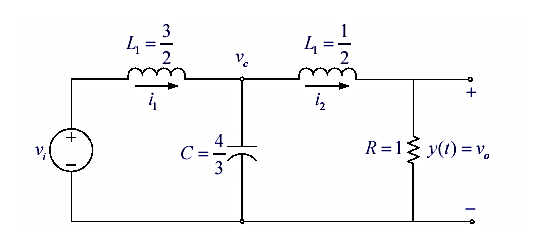
\includegraphics[width=3.4in]{thirdorderLPfilter}
\caption{\footnotesize
        Third-order low-pass filter
        \label{fig.statespacelab.thirdorderLPfilter}
        }
\end{figure}

\begin{enumerate}
\item The circuit shown in Figure~\ref{fig.statespacelab.thirdorderLPfilter}
    is a third-order Butterworth filter.  Select appropriate state variables and obtain the state and output equations.  Treat the output, $y(t)$, as the voltage across the resistor.\\
    The general idea is to express the differential equations that describe the circuit as a system in matrix form.  With this in mind, the following notes may be helpful:
        \begin{itemize}
        \item In the absence of all capacitor and voltage source loops and all
            inductor and current source cut-sets, the number of state variables is equal to the number of energy storage elements.
        \item Appropriate state variables may be the voltage across the
            capacitor and the current in the inductors.
        \item Write a node voltage equation for every node touching a
            capacitor.  Also, consider writing loop equations in terms of the inductor currents for loops containing inductors.
        \end{itemize}
\item Write a script m-file and use the Control System Toolbox functions
    \verb=ss= and \verb=ltiview= to form the state model and its step response.  Also, use \verb=ss2tf= to obtain the filter's transfer function.\\
    Run the m-file.  Right-click on the LTI Viewer and use Characteristics to display all of the time-domain specifications.  Be sure to look at both the step- and impulse-response plots.  \\
    Right-click on the LTI Viewer again and from the Plot Type list, select ``Bode.''  From the File menu, select ``Print to Figure'' to obtain a figure plot capable of being edited.  Click on the magnitude response and hold and drag to display the corner frequency at -3~dB.  Now drag to display the attenuation at 10~rad/sec.\\
    Summarize the step response characteristics and the filter transfer function.  Comment on the filter frequency response characteristics.
\end{enumerate}

\Closesolutionfile{StaVarSolutions}
% LAB 3:
% Modeling and Simulation Case Studies

\Opensolutionfile{ModSimSolutions}
% \begin{solmodsim}
% \end{solmodsim}

\chapter{Modeling and Digital Simulation Case Studies} \label{ch.ModSim}

One of the objectives of this session is to get you acquainted with the basics of Simulink, a graphical modeling, simulation, and prototyping environment used extensively in industry.  We will not be able to cover the vast capability of Simulink with a few examples; you are encouraged to explore various features and graphical programming techniques on your own.
\par
The other objectives of this lab are to find the mathematical model for some basic physical systems, to obtain a digital simulation diagram for the resulting differential equations, and to obtain the system's step response and investigate the effect of damping on the system response.

\section{Pre-Lab Reading}
Read the following introductory material.  More help can be found in Appendix~\ref{app.statespace}.
\par
The dynamic performance of physical systems is obtained by utilizing the related physical laws governing them.  Many dynamic systems contain energy storage elements such as masses and springs (in mechanical systems) or inductors and capacitors (in an electric circuit).  The principle of conservation of energy prohibits instantaneous changes in the state variables. Therefore, the system will go through some transients before settling to their steady-state values.
\par
All physical systems are nonlinear to some extent.  In order to model the system with linear time-invariant differential equations (for transfer function or state space representations), the system must first be linearized.  Alternatively, its range of operation may be confined to a linear range.
\par
The next step in designing a practical control system is to simulate the model on a computer to obtain the system response to various signals and disturbances.  Then we can introduce appropriate controllers to achieve the desired system response.  This process of design and analysis is repeated until a satisfactory control system is obtained and then the design may be implemented on the hardware.
\par
One of the most powerful tools for modeling and simulation of dynamic systems is Simulink, a toolbox extension of MATLAB.  Simulink's strongest selling point is that it is very visual and intuitive.  A system in block diagram representation is built easily and the simulation results are displayed quickly.  Simulation algorithms and parameters can be changed in the middle of a simulation with natural results, thus providing the student with a readily accessible learning tool for simulating many of the operational problems found in the real world.
\par
Simulink is particularly useful for studying the effects of nonlinearities on the behavior of the a system.  As such, it is also an ideal research tool.  Simulink has many advanced features for simulating a complex control system, such as the creation of new subsystem blocks and \uline{masking blocks} through m-files, C programs, or other Simulink models for easy integration in your system's model.  This allows an extension of the Simulink graphical functions to suit your own needs of analysis and design.  The Simulink demos and User's Guide are very helpful in explaining the advanced usage and extension of the Simulink block library.  For more information on Simulink, see Chapter~1 in \cite{saadatbook} or browse \cite{saadatsite}.

\section{Laboratory Procedure}

\begin{casestudy}{Mechanical Translational System} \label{cs.mechtrans}
Consider a simple mechanical system consisting of a mass, spring, and shock absorber---known as a \textit{dashpot} or \textit{piston}---shown in Figure~\ref{fig.mechdiagram}.  In the figure, $M$ is the mass, $B$ is the damping coefficient, $k$ is the spring constant, $f(t)$ is the external force, and $x(t)$ is the displacement of the mass.  Three forces (and inertia) influence the motion of the mass, namely the applied force, the damping force, and the spring force as shown in the free-body diagram in Figure~\ref{fig.freebody}.

\newsavebox{\tempbigA}
\newsavebox{\tempsmallA}
\begin{figure}[bht]
    \centering
    \sbox{\tempbigA}{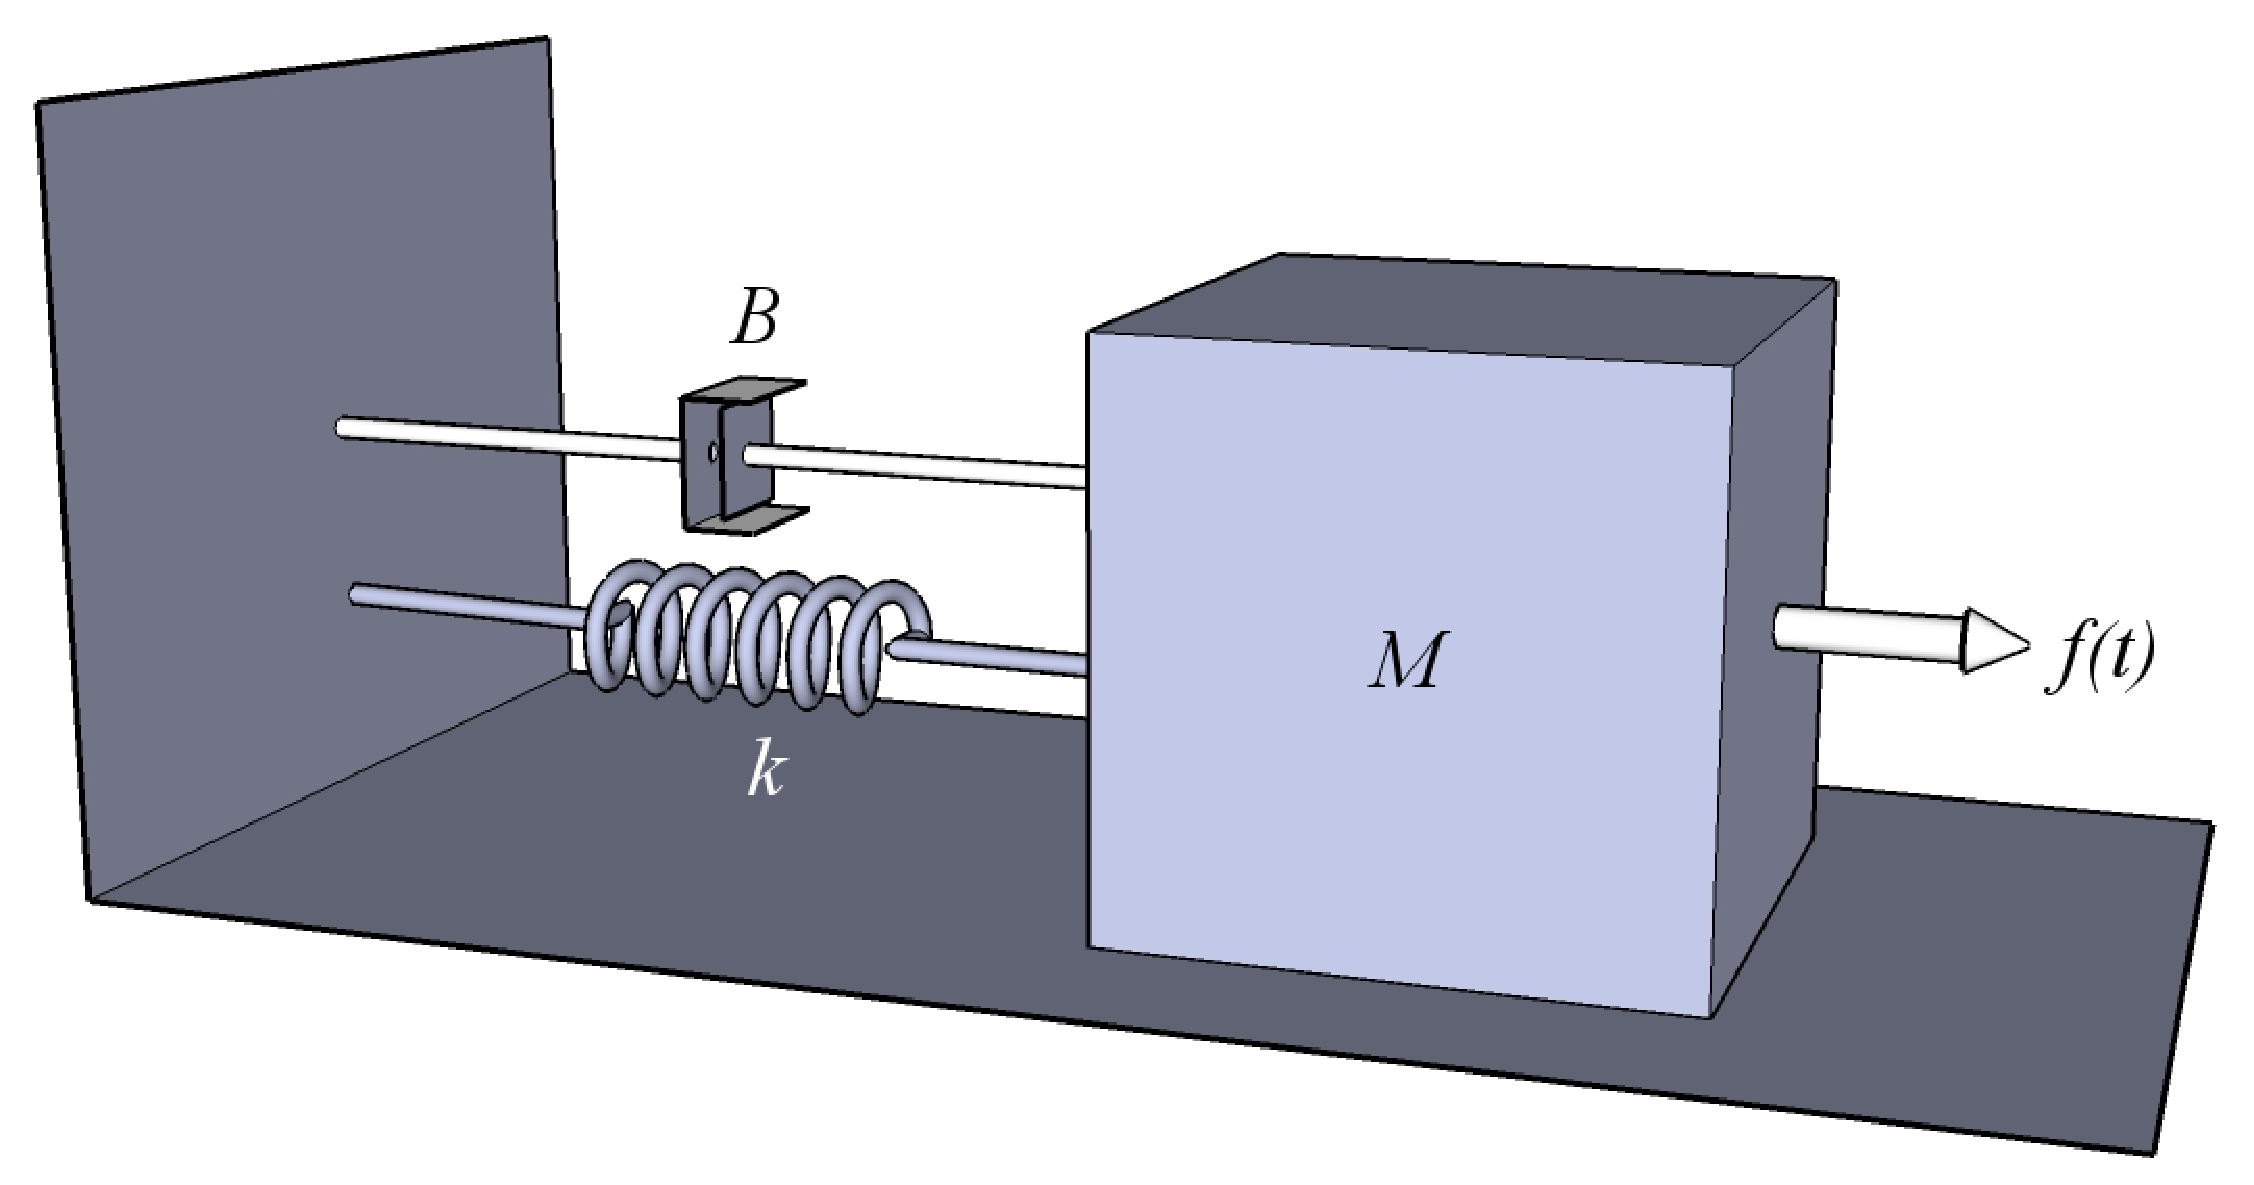
\includegraphics[width=.6\textwidth]{mechdiagram}}
    \sbox{\tempsmallA}{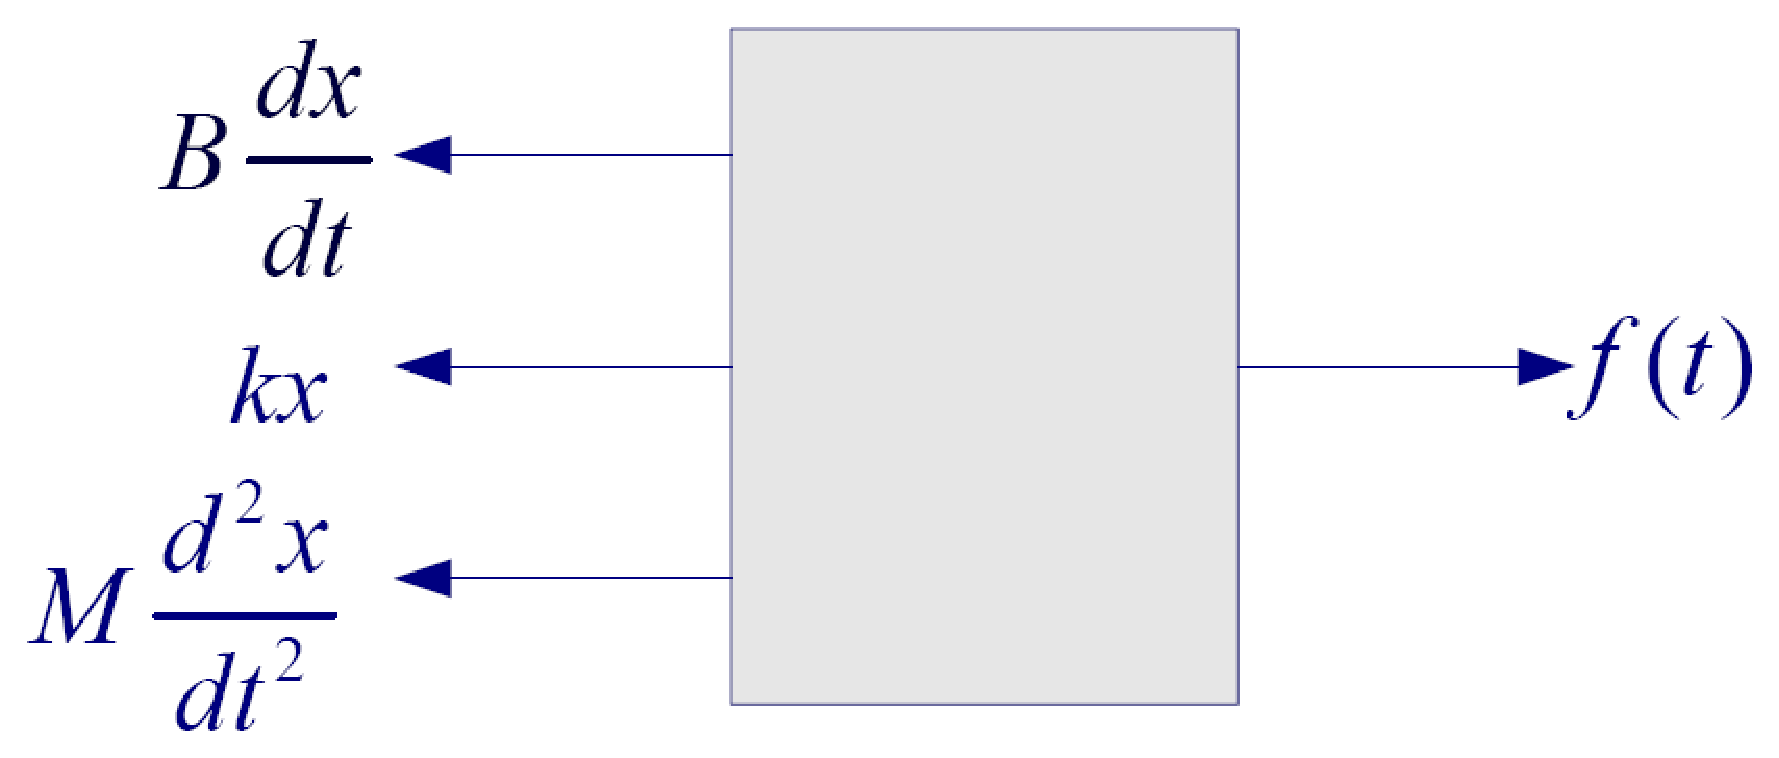
\includegraphics[width=.35\textwidth]{mechfreebody}}
    \newlength{\subfigoffsetA}
    \setlength{\subfigoffsetA}{0.5\ht\tempbigA}
    \addtolength{\subfigoffsetA}{-0.5\ht\tempsmallA}
    \subfloat[
            Mechanical translational system
            \label{fig.mechdiagram}
            ]{
            \usebox{\tempbigA}
            }
    \hfill
    \subfloat[
            Free-body diagram
            \label{fig.freebody}
            ]{
            \raisebox{\subfigoffsetA}{\usebox{\tempsmallA}}
            }
    \caption{}
\end{figure}

Applying Newton's Second Law, we have 
\begin{equation}
    M\frac{d^2 x(t)}{dt^2} + B\frac{d x(t)}{dt} + kx = f(t)
        \label{eq.mechfreebody}
\end{equation}
The transfer function model is obtained by taking the Laplace transform (with zero initial conditions), which results in:
\begin{equation}
    G(s) = \frac{X(s)}{F(s)} = \frac{1}{Ms^2 + Bs + k}
        \label{eq.mechtf}
\end{equation}
You may note that for complicated mechanical systems, it is easier to draw the electric circuit force-voltage analogy in place of the free-body diagram.  In the force-voltage analogy, mass ($M$) is analogous to inductance, spring compliance ($1/K$) is analogous to capacitance, damping coefficient ($B$) is analogous to resistance, and velocity ($\dot{x}$) is analogous to current.  The key point in drawing the electric circuit analogy is to identify the displacement or velocity of each element and draw the circuit accordingly.  The circuit can be drawn in the s-domain to find the transfer function or in the time domain which is suitable for obtaining the state space model.  The electric circuit analogy for this mechanical system is shown in Figure~\ref{fig.mechelecanalogy}.

\begin{figure}[bht]
\centering
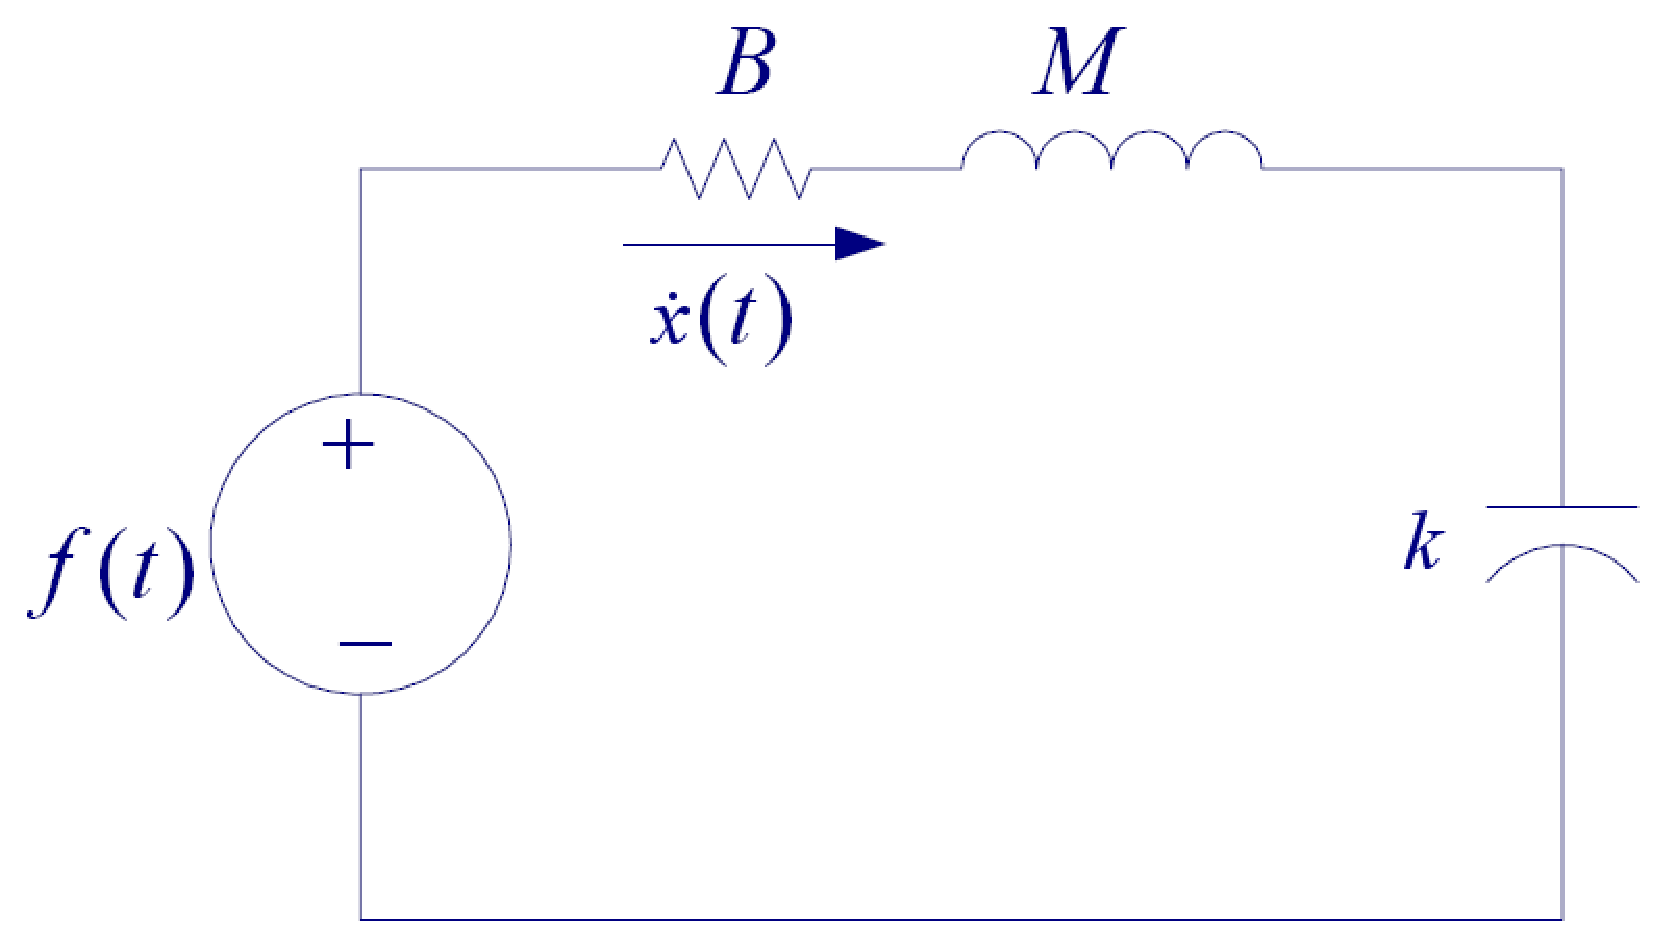
\includegraphics[width=.5\textwidth]{mechelecanalogy}
\caption{\footnotesize
        Electric circuit analogy for the mechanical system in Fig.\ \ref{fig.mechdiagram}
        \label{fig.mechelecanalogy}
        }
\end{figure}

With Kirchhoff's voltage law applied to the electric circuit, we get
\begin{equation}
    M\frac{d\dot{x}(t)}{dt} + B\dot{x}(t) + k\int_0^t \dot{x}(\sigma) = f(t)
\end{equation}
which is of course mathematically equivalent to (\ref{eq.mechfreebody}).  Equation~(\ref{eq.mechfreebody}) can also be written in state space form by selecting the two state variables as displacement and velocity: $x_1(t)=x(t)$ and $x_2(t) = \dot{x}(t)$.  The first-order differential equations then become
\begin{equation} \label{eq.mechdiff}
\begin{split}
    \frac{dx_1(t)}{dt} & = x_2(t) \\
    \frac{dx_2(t)}{dt} & = \frac{1}{M}f(t) - \frac{k}{M}x_1(t) - \frac{B}{M}x_2(t)
\end{split}
\end{equation}
For convenience, we will define multiple outputs: $y_1 = x_1(t)$ and $y_2 = x_2(t)$.  Thus the state space expression of this system is
\begin{equation}
\begin{split}
    \left[ \begin{array}{c} \dot{x}_1(t) \\ \dot{x}_2(t) \end{array} \right]
    & = 
    \left[ \begin{array}{cc} 0 & 1 \\ -\frac{k}{M} & -\frac{B}{M} \end{array}
        \right]
    \left[ \begin{array}{c} x_1(t) \\ x_2(t) \end{array} \right]
    +
    \left[ \begin{array}{c} 0\\ \frac{1}{M} \end{array} \right]
    f(t)
    \\
    \left[ \begin{array}{c} y_1(t) \\ y_2(t) \end{array} \right]
    & =
    \left[ \begin{array}{cc} 1&0\\0&1 \end{array} \right]
    \left[ \begin{array}{c} x_1(t) \\ x_2(t) \end{array} \right]
\end{split}
\end{equation}
The simulation diagram for Equations~(\ref{eq.mechdiff}) is shown in Figure~\ref{fig.mechsimdiagram}

\begin{figure}[bht]
\centering
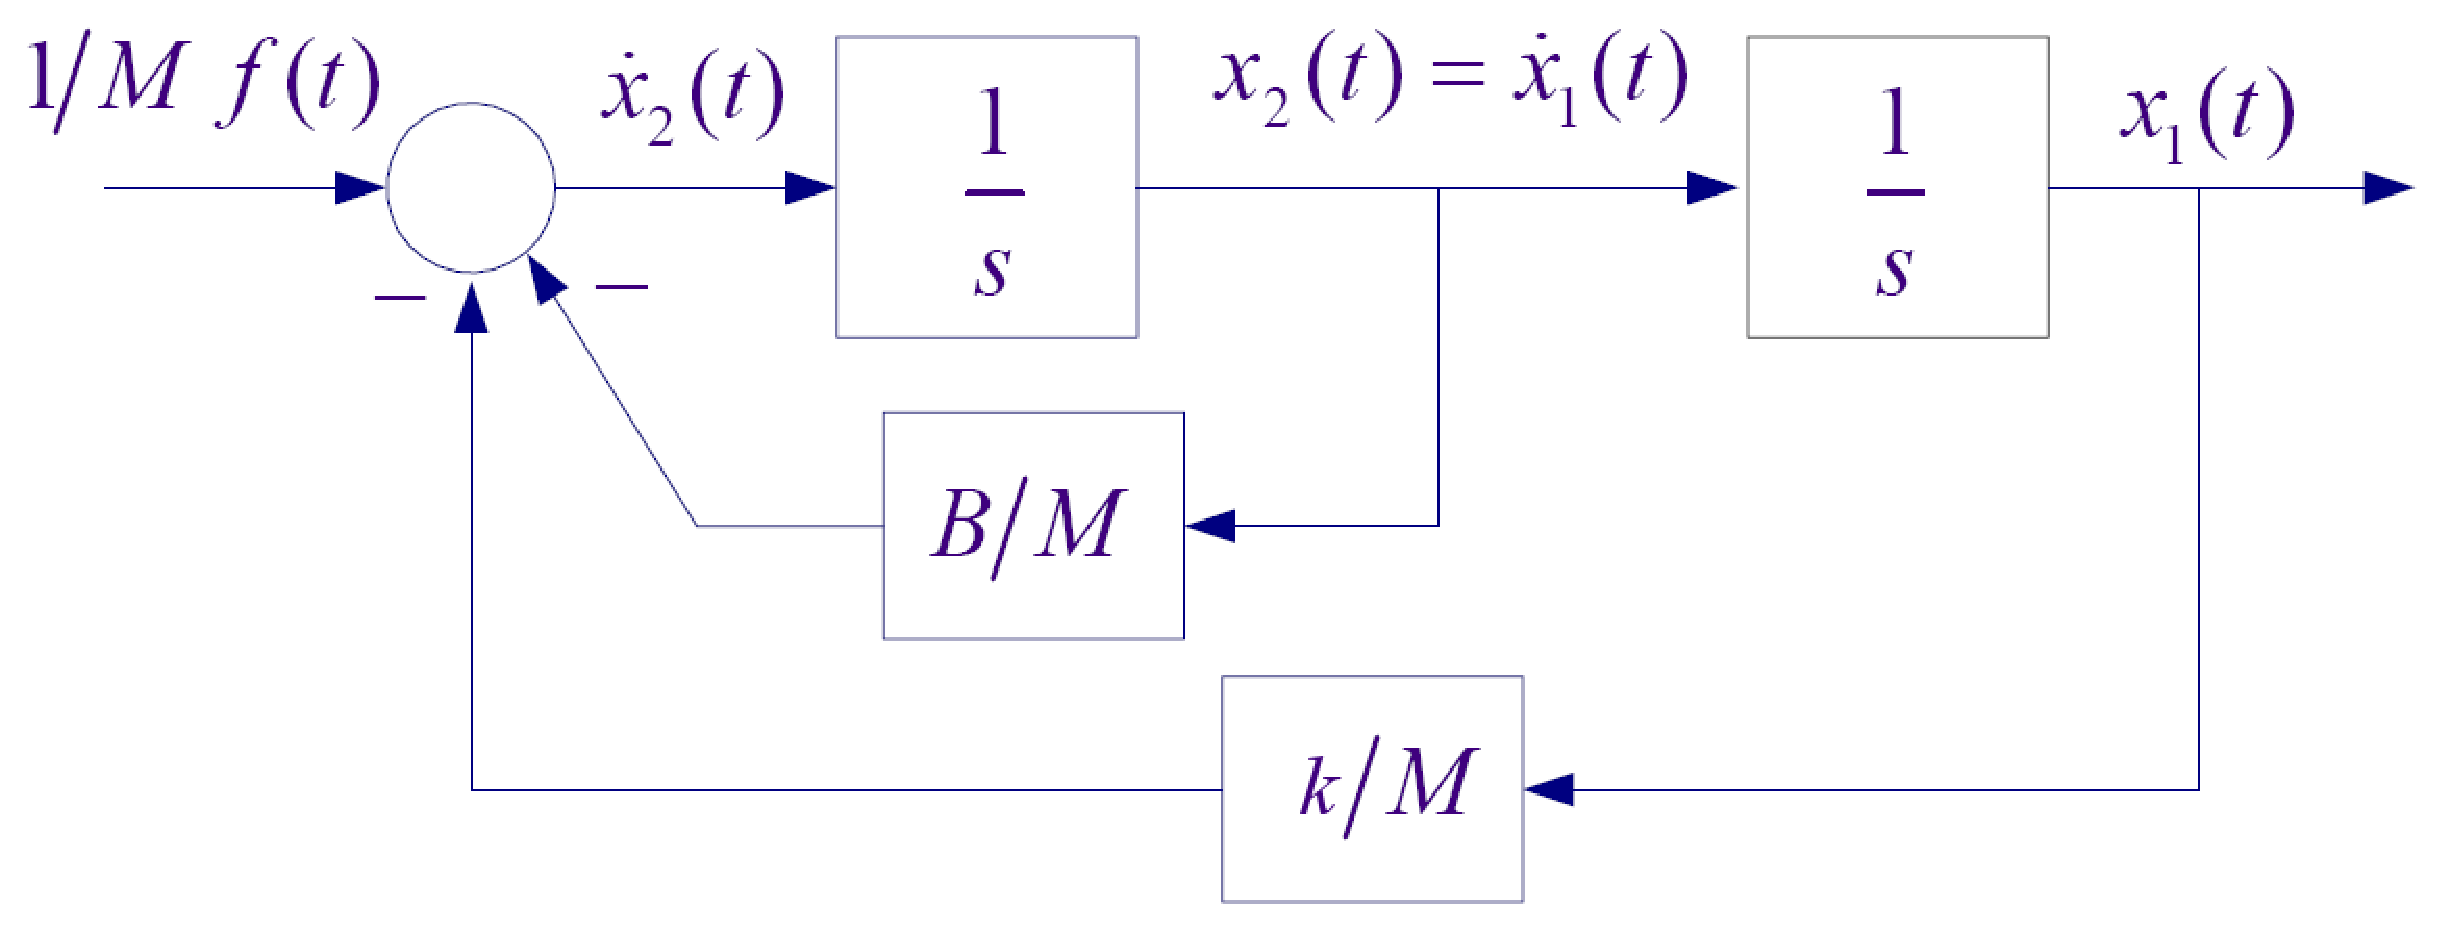
\includegraphics[width=.6\textwidth]{mechsimdiagram}
\caption{\footnotesize
        Simulation diagram for the mechanical system in Case Study~\ref{cs.mechtrans}
        \label{fig.mechsimdiagram}
        }
\end{figure}

With the system initially at rest, a constant force of $f(t) = 32$~Newtons is applied at time $t=0$.  The system in question has a mass of $2$~kg and a spring constant of $32\mbox{ kg}/\mbox{s}^2$.  We are told that the damping coefficient, $B$, may be adjusted to obtain a desirable response.
\par
The system's characteristic equation---from Eq.\ (\ref{eq.mechtf})---is given by
\begin{equation}
    s^2 + \frac{B}{M} s + \frac{k}{M} = 0
\end{equation}
which may be compared to the standard second-order transfer function
\begin{equation}
    s^2 + 2 \zeta \omega_n + \omega_n^2 = 0
\end{equation}

\begin{enumerate}
\item
    \textbf{Perform the following analysis:}
    \begin{enumerate}
    \item
        The dashpot damping is adjusted to $B = 2\mbox{ Ns/m}$.  Determine the natural frequency of oscillation ($\omega_n$), damping ratio ($\zeta$), percent overshoot ($PO = 100e^{-\frac{\zeta\pi}{\sqrt{1-\zeta^2}}}$), peak time ($t_p = \frac{\pi}{\omega_n \sqrt{1-\zeta^2}}$), and settling time ($t_s \approx 4\tau$).
    \item
        jk;asdf
    \end{enumerate}
\item
    ;lakjdf
\end{enumerate}

\end{casestudy}
\begin{casestudy}{
Simple Pendulum}
\label{cs.simplepend}

\end{casestudy}


\begin{thebibliography}{9}
    \bibitem{saadatbook} Hadi Saadat.  Computational Aids in Control Systems Using MATLAB.  McGraw-Hill.  1993.
    \bibitem{saadatsite} Hadi Saadat website. http://people.msoe.edu/~saadat/matlab.htm
\end{thebibliography}

\Closesolutionfile{ModSimSolutions}

% Lab 4:
% DAQ
\chapter{Introduction to Data Acquisition and Real-Time Control}

The objectives of this laboratory session are:
\begin{itemize}
\item
    Gain familiarity with the Quanser MultiQ8 board and WinCon Software.
\item
    Understand the basic input/output (I/O) connections.
\item
    Create a WinCon application for the encoder and measure the encoder angle.
\item
    Create a WinCon application to run the motor and measure the tachometer and potentiometer signals.
\end{itemize}

\section{Pre-Lab Assignment}

Read the following introduction and skim the wiring and connection diagrams in this lab handout.
\par
Digital control of a continuous-time systems has become very popular as the price and reliability of digital computers has improved.  Digital sensors (like thermocouples in thermostats) and a computer (like an integrated circuit)  perform calculations to emulate the analog controllers (like bi-metal strips) they replace.  Very complicated control structures can be implemented easily using a digital controller, whereas an analog controller would require complex hardware.  Digital controllers are more adaptable to parameter changes than their analog counterparts.  Furthermore, analog emulation and real-time control provide advanced features such as adaptive self-tuning, multivariable control, expert systems, and the ability to communicate over a local area network.
\par
Typically, the computer replaces the cascade controller.  The measured data is converted from analog to digital form by the analog-to-digital converter (ADC).  This is accomplished by the data acquisition system (DAQ) which is the ``eyes and ears'' of the digital computer.  The computer receives and manipulates the signal in digital (binary) form, and the output is then converted to analog by the digital-to-analog converter (DAC).  This process is the ``hands and arms'' of the computer.
\par
The full scale output is usually determined by an external reference voltage.  The DAC resolution is defined as the smallest possible change in output.  For an $N$-bit converter the resolution is given by Eq.\ (\ref{eq.outputresolution}).
\begin{equation}
    \mbox{Resolution } = \frac{100}{2^N}\%
    \label{eq.outputresolution}
\end{equation}
For example, the resolution of a $10$-bit DAC is
\begin{equation*}
    \frac{100}{2^{10}} = \frac{100}{1024} = 0.09766\%
\end{equation*}
The resolution of an ADC is defined as the smallest detectible change in input, which is also given by (\ref{eq.outputresolution}).
\par
When the computer reacts to external events as they occur, it is referred to as \uline{real-time} control.  An important consideration in real-time control is the update rate.  During one controller cycle, three things must happen before the next cycle can begin:
\begin{inparaenum}[1)]
\item
    Sensors are read (ADC inputs),
\item
    The microprocessor computes updated commands, and
\item
    The commands are converted to analog signals (DAC outputs).
\end{inparaenum}
Between cycles, the commands outputs are held constant.  If the controller is updated every 0.01 seconds, the output of the controller would look like a staircase with steps 0.01 seconds wide.  As expected, the faster the dynamics of the system being controlled (pouring water versus pouring molasses), the faster the update rate must be.
\par
Modern real-time control systems use computer aided software engineering (CASE) such as MATLAB's Real-Time Workshop to automatically generate C code from a graphical control model (like Simulink).  Often the sensors or other components of the DAQ system are proprietary.  Vendors now provide Simulink blocks along with their hardware in order to ease the graphical modeling of their product.
\par
In this lab, we will focus on gaining familiarity with the MultiQ8 DACB and WinCon software.  In addition, you will explore the effects of A/D and D/A conversion that are built into the MultiQ8 board through which all the control signals pass.

\section{Laboratory Procedure}
This experiment requires four items to be connected; the parenthetical comments are what these devices will be commonly referred to hereafter:
\begin{enumerate}
\item SRV-02 Motor (plant)
\item MultiQ8 data acquisition board (DAQ board)
\item Universal power module (UPM)
\item computer (CPU)
\end{enumerate}

\subsection{Wiring Connections}
The proper connection of these elements is crucial---and particularly confounding in the tight spaces on the lab bench.  The connections are detailed in Table~\ref{tab.daqconnections} and pictured as a whole in Figure~\ref{fig.daqconnections}.

\begin{table}[bht]
\centering
\renewcommand{\arraystretch}{1.1}
\begin{tabular}{c | c | c | l}
    \textit{Order}  &   \textit{From}   &   \textit{To} & \multicolumn{1}{c}{\textit{Cable}} \\
        \hline \hline
    1   &   Plant ``motor''     &   UPM ``To Load'' &   4-DIN to 6-DIN \\
    2   &   Plant ``tach''      &   UPM ``S3''      &   6-DIN mini to 6-DIN
                                                        mini \\
    3   &   Plant potentiometer ``S1 \& S2''
                                &   UPM ``S1 \& S2''&   6-DIN mini to 6-DIN
                                                        mini \\
    4   &   DAQ ``Encoder 0''   &   Plant ``Encoder''&  5-DIN to 5-DIN \\
    5   &   DAQ ``Analog Output 1''
                                &   UPM ``From D/A''&   Phono to 5-DIN \\
    6   &   DAQ ``Analog Input 1--4''
                                &   UPM ``To A/D''  &   4xRCA to 5-DIN \\
    7   &   DAQ ``Cable 1--3''  &   CPU             &   Serial bus ribbons
\end{tabular}
\caption{\footnotesize
        Wiring connections for basic experimental setup
        \label{tab.daqconnections}
        }
\end{table}

\begin{figure}[bht]
\centering
\includegraphics[height=.9\textheight]{2590Setup}
\caption{\footnotesize
        Proper connections for the basic experimental setup.  Note the serial bus ribbons are not shown but should connect to the DAQ board as indicated.  They are size-keyed so that it is clear where they plug in.
        \label{fig.daqconnections}
        }
\end{figure}

Do not power up the amplifiers.  Make sure the LED on the DAQ board is illuminated.  If it is not, then the fuse needs replacement.  Contact the instructor.
\par
Close-up photographs of the equipment with connection details are provided in Figure~\ref{fig.equipmentcloseups}.

\begin{figure}[thb]
\centering
\subfloat[
    \footnotesize
    SRV-02 Plant.  (A) goes to UPM ``To Load.''  (B) goes to UPM ``S3.''  (C) goes to DAQ ``Encoder'' position 0.  (D) goes to UPM ``S1 \& S2.''
    ]{
    \includegraphics[width=.45\textwidth]{2594Plant}
    }
\hfill
\subfloat[
    \footnotesize
    MultiQ8 Data Acquisition (DAQ) board.  (E) goes to Plant ``Encoder.''  (P) goes to UPM ``From D/A.''  (RWYK) bundle and go to UPM ``To A/D.''
    ]{
    \includegraphics[width=.5\textwidth]{2607MultiQ}
    }
\newline
\subfloat[
    \footnotesize
    Universal power module (UPM).  (A) goes to DAQ ``Analog Outputs'' position 0.  (B) goes to Plant ``S1/S2.''  (C) goes to Plant ``Tach.''  (D) goes to Plant ``Motor.''  (E) goes to DAQ ``Analog Inputs'' positions 1 (yellow), 2 (white), 3 (red), and 4 (black).
    ]{
    \includegraphics[width=.75\textwidth]{2596UPM}
    }
\caption{\footnotesize
        Equipment connection details
        \label{fig.equipmentcloseups}
        }
\end{figure}

\clearpage
\subsection{Create the Simulink Model}
The encoder is used to provide the digital phase information.  Start MATLAB, launch Simulink, and open a new model.  From the Simulink Library, get the Encoder Input block from the Quanser Toolbox/Quanser Consulting MultiQ8 Series folder as seen in Figure~\ref{fig.multiq8libraryblock}.

\begin{figure}[bht]
\centering
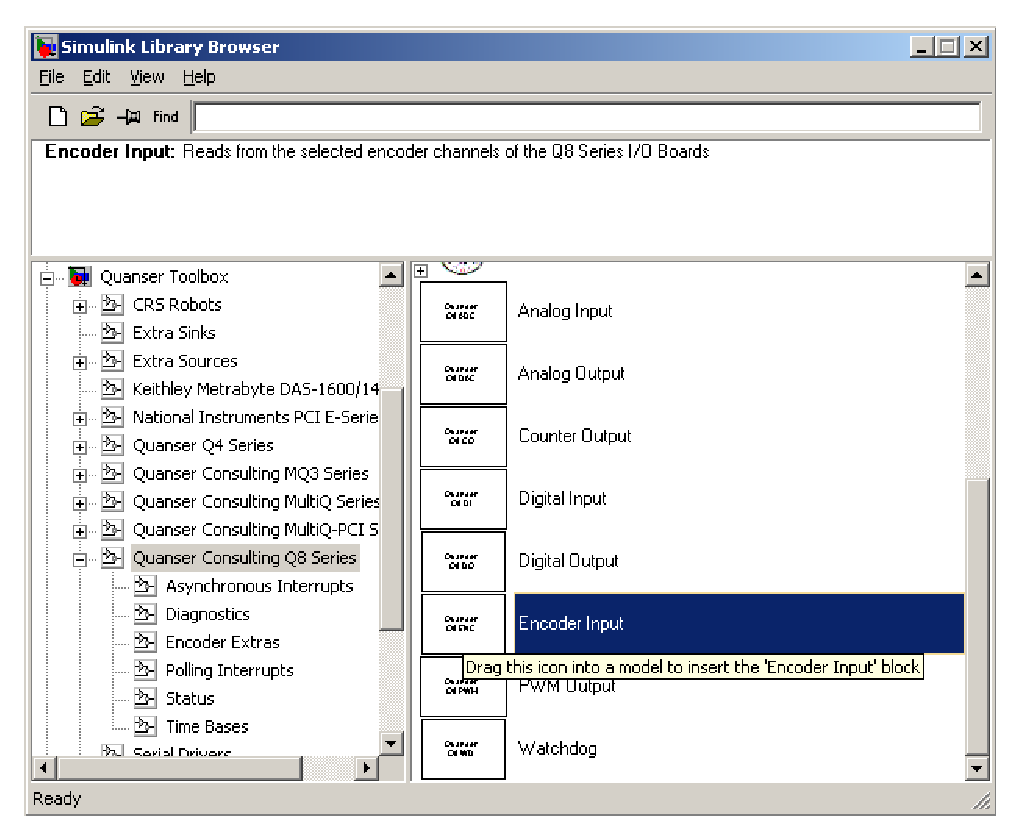
\includegraphics[width=.65\textwidth]{QuanserToolboxScreenshot}
\caption{ \footnotesize
        Simulink library including the proprietary Quanser Q8 toolbox
        \label{fig.multiq8libraryblock}
        }
\end{figure}

Draw a Simulink diagram as shown in Figure~\ref{fig.encodermeasure}.  The encoder input is connected to Encoder~0 on the MultiQ wiring diagram.  Double-click on the Encoder input block to open its dialog box and set the ``Channel to Use'' to 0.  Save the model.

\begin{figure}[bht]
\centering
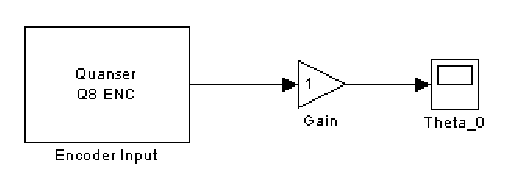
\includegraphics[width=.5\textwidth]{encoderonly}
\caption{\footnotesize
        Simulink diagram for encoder experiment
        \label{fig.encodermeasure}
        }
\end{figure}

There are a few tips for drawing Simulink models.  It is often easiest to place all the blocks in rough positions first.  To connect blocks, try this: Click on the origin block, hold the \textit{Control} key, and click on the destination block.  This can be repeated until all blocks are appropriately connected.
\par
Also, it is sometimes helpful to rename blocks so that we can recognize them later.  For example, Simulink models often have many Gain blocks.  Instead of having them named Gain, Gain1, Gain2, and so on, single-click on the name in the model and rename them with something more descriptive.

\subsection{Compiling the Model}
If you choose to use a mobile machine to run the experiments, read the following.  If not, please skip the boxed material.
\par \noindent
\begin{center} \setlength{\fboxrule}{0.5pt}
\fbox{\parbox{.9\textwidth}{\vspace{-6pt} \begin{flushleft}
\textbf{Optional Instructions for Remote Connections} \end{flushleft}
\parbox{.9\textwidth}{ \small
Before you run any real-time code, you need to launch the WinCon server and connect to the client PC where the experiment is going to run.  Ensure that WinCon Client is running on the PC you want to connect to.  Start the WinCon server on your laptop and then use Client\textrightarrow Connect as shown in Figure~\ref{fig.clientconnect}.  In the dialog box, enter the proper client workstation IP address (The station IP addresses are s312-1 to s312-10).
}
}
}
\end{center}

\begin{figure}[bht]
\centering
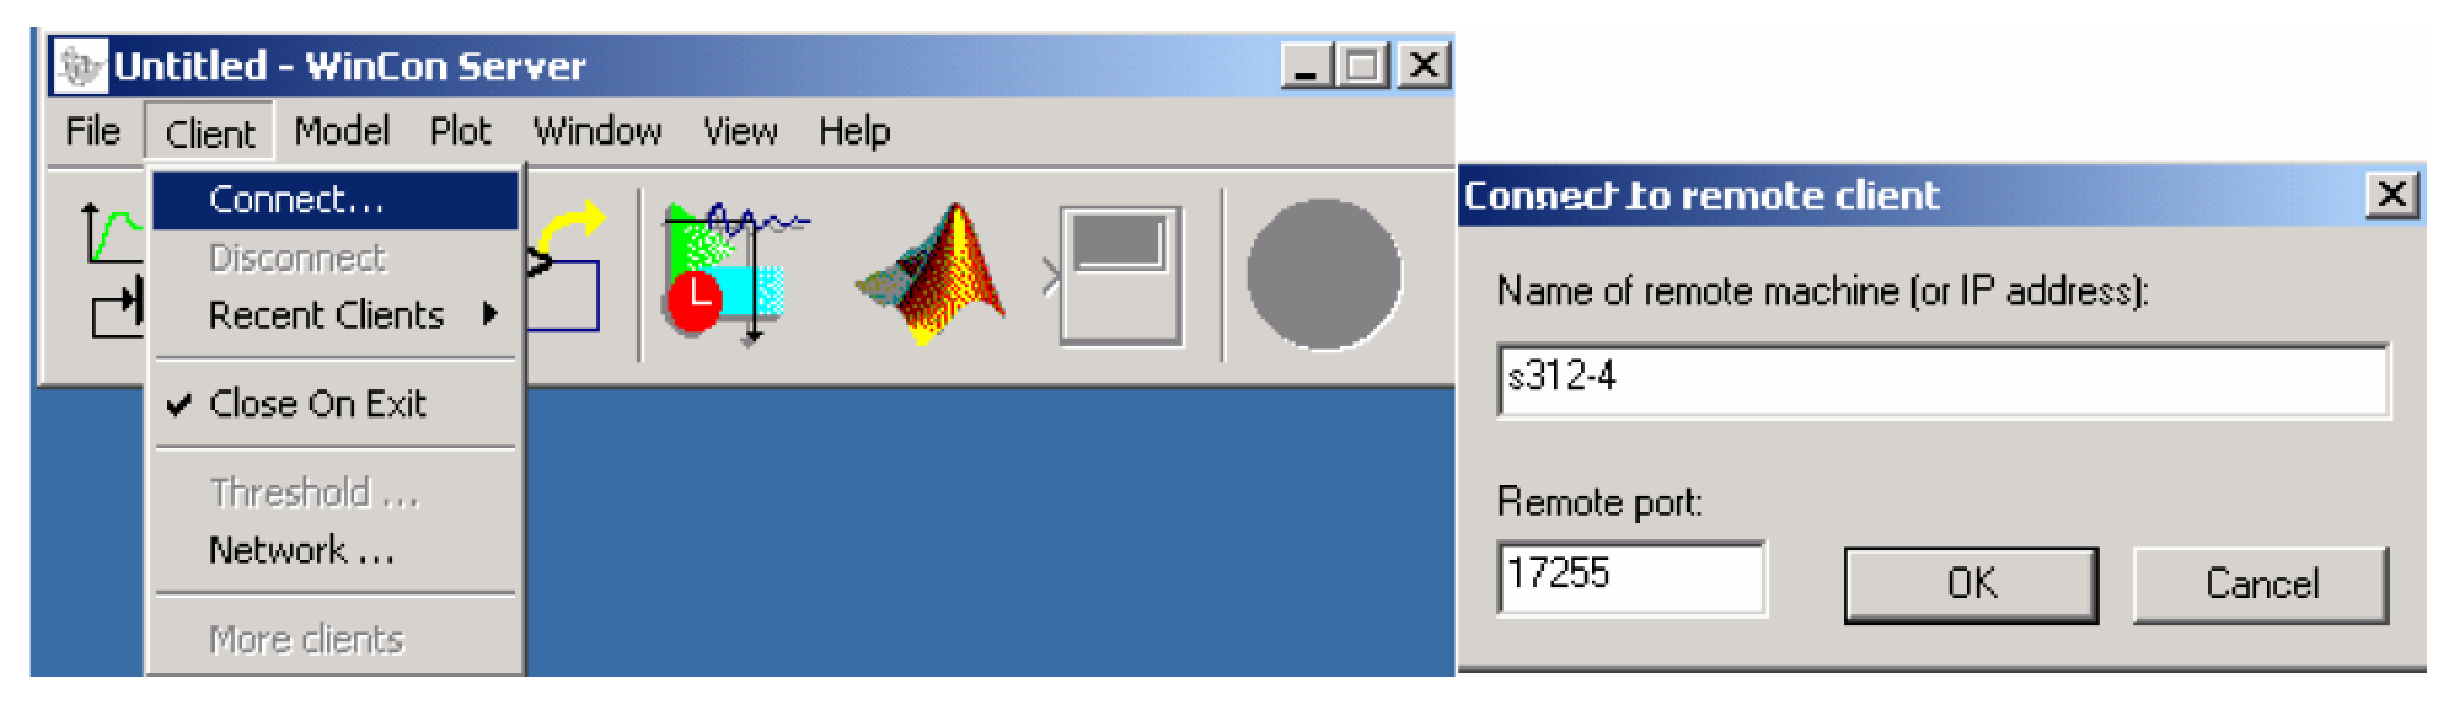
\includegraphics[width=.6\textwidth]{clientconnect}
\caption{ \footnotesize
        Remote connection to the client that is running the experiment
        \label{fig.clientconnect}
        }
\end{figure}

In order to run the simulation in real-time, you must first build the code for it.  This is done using the WinCon\textrightarrow Build option seen in the diagram in Figure~\ref{fig.winconbuild}.  However, there are several simulation parameters that need to be set before building the model.

\begin{figure}[bht]
\centering
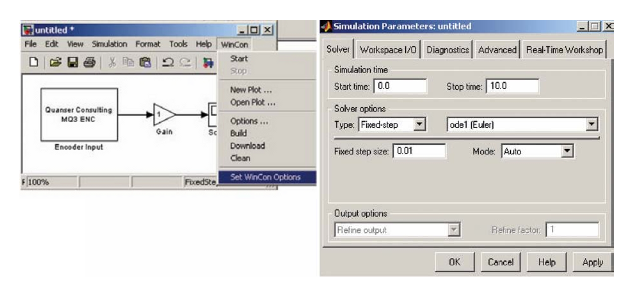
\includegraphics[width=.75\textwidth]{winconbuild}
\caption{ \footnotesize
        WinCon dropdown menu in Simulink.  Simulation parameters are set as shown in this menu under ``Set WinCon Options.''  When ready, the model is built with WinCon\textrightarrow Build.
        \label{fig.winconbuild}
        }
\end{figure}

Select WinCon\textrightarrow Options to open the Simulation Parameters dialog box.  Choose the Solver tab and set the sampling rate on the controller to a fixed step size of 0.01 seconds.  Also, select ``ode4 (Runge-Kutta)'' as the integration method.  In the Simulation dropdown menu, set the model to ``External.''
\par
Now click WinCon\textrightarrow Build.  This will generate the code and compile it.  It may take a while depending on the machine you are working on.  When the compile is done, the code will download to the WinCon Client.  You can now use the WinCon Server to start and stop real-time code.  These two windows are shown in Figure~\ref{fig.clientserver}.  If it is not open already, open the WinCon Server; we will need it in the next section.

\begin{figure}[hbt]
\centering
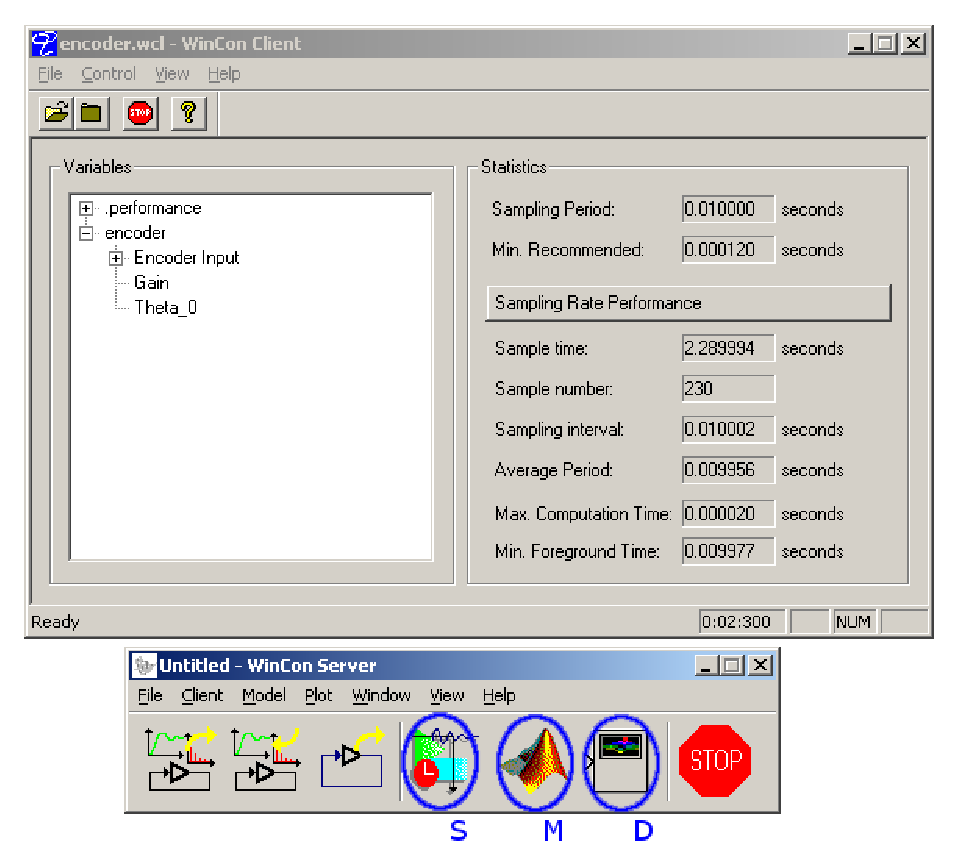
\includegraphics[width=.6\textwidth]{clientserver}
\caption{ \footnotesize
        WinCon Client (above) and Server (below).  The (S) button brings up the pertinent Simulink model, (M) brings up the MATLAB window, and (D) opens the WinCon Display Dialog.
        \label{fig.clientserver}
        }
\end{figure}

\subsection{Encoder Signal}
Now we are ready to see the real-time code in action.  To visualize the data, WinCon offers the Display button next to the Start/Stop button.  This links to all of the output displays we built into our Simulink model.  For this experiment, we should have a trace available called \textit{Theta\_0}.  Open this trace and start the experiment.
\par
With WinCon running, rotate the gears of the plant (by hand) and observe the real-time trace.  The default time span is five seconds.  To increase this, go to Update\textrightarrow Buffer and change to the desired amount.  You can, of course, at any time stop the experiment by clicking on the big red Stop button in the WinCon Server.
\par
In a blank trace window, rotate the big (central) gear 45\textdegree\ counterclockwise (ccw), then back 90\textdegree\ clockwise (cw), and then back to the starting position.  Stop the experiment.  There is no need to be terribly exact, we are primarily concerned with the sign of the encoder for this motion.
\par
Hopefully your trace will look something like Figure~\ref{fig.angletrace}.  If your counterclockwise motion produced negative data points, you will need to change the gain block in your Simulink diagram from $+1$ to $-1$.  It is important for this experiment and subsequent ones that counterclockwise motion have a positive sign and the opposite for clockwise motion!

\begin{figure}[bht]
\centering
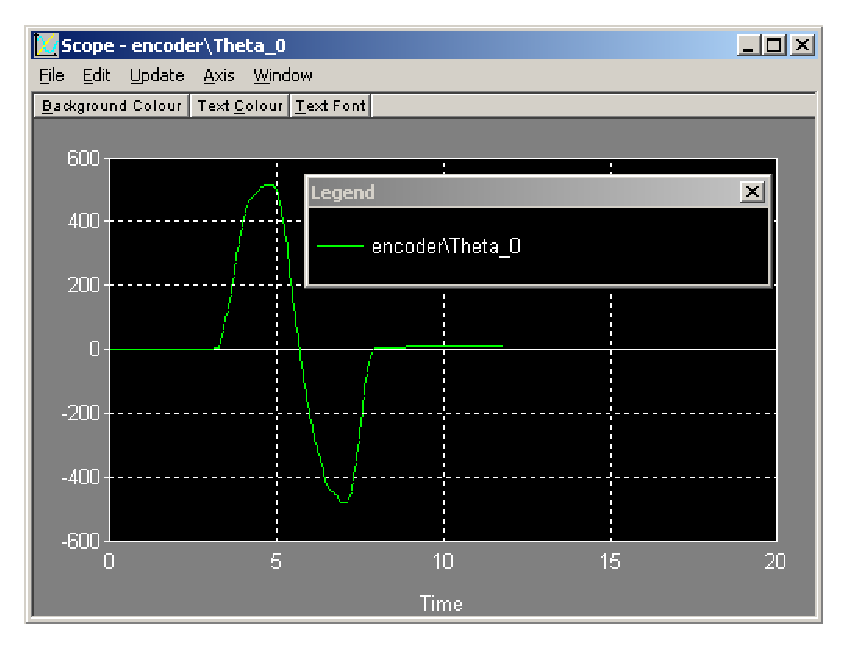
\includegraphics[width=.6\textwidth]{angletrace}
\caption{\footnotesize
        Sample trace of the encoder output.  Counterclockwise motion corresponds to positive data, so the Simulink gain block is correctly configured.
        \label{fig.angletrace}
        }
\end{figure}

To add a legend to the trace, use the Window dropdown menu.
\par
Here it is important to note that we can import the data seen by WinCon to MATLAB.  In the trace window, the File\textrightarrow Save menu allows us to export the data points as an m-file, a mat-file, or directly to the MATLAB workspace as variables.
\par
With MATLAB, observe the numerical data recorded for the $\pm$45\textdegree\  run.  In particular, note the following:
\begin{enumerate}
\item
    Does the data start and end at zero?  Why is this?
\item
    What are the maximum and minimum data points?  Why are they not $+45$ and $-45$?
\item
    How could you calculate the speed at which you turned the gears from this data?  What would the units be?
\end{enumerate}

We will focus on Item 2.  The others are appropriate to be addressed in the lab report.
\par
As you noted, the encoder did not record 45\textdegree---or anything close---when you turned the gears by about that amount.  This is because the encoder uses proprietary units called \uline{counts}.  The encoder measures 1024 counts per revolution in quadrature.  Thus a rotation of 360\textdegree\  results in $1024\times4 = 4096$ counts.  This means that the resolution of the encoder is $360/4096 = 0.087890625$\textdegree.
\par
In order to have future data in degrees, change the gain block in the Simulink model (Fig.\ \ref{fig.encodermeasure}) to $360/4096$ with the appropriate sign.

\subsection{Sensor Calibration}
Now that we have some experience with drawing a Simulink model, building the real-time code, and interfacing with WinCon, we are ready to observe and calibrate the equipment.  The motor on the plant is driven by an amplifier that can deliver the desired power to it.  In order to drive a voltage to the motor, we need to output the desired voltage to the correct D/A channel.  From the wiring we performed (see Table~\ref{tab.daqconnections} and Fig.\ \ref{fig.daqconnections}), we know that DAC Channel 1 drives the UPM, which in turn drives the motor.
\par
Click File\textrightarrow New in WinCon---do not save anything.  Start a fresh Simulink diagram (see Figure~\ref{fig.calibratemodel}).  Use the same simulation parameters from the encoder model, except change the fixed step size to 0.001~seconds.  Connect a constant block via a gain to the Quanser Analog Output block.  This will output a constant voltage to the channel specified in the output block's parameters (double-click).
\par

\begin{figure}[bht]
\centering
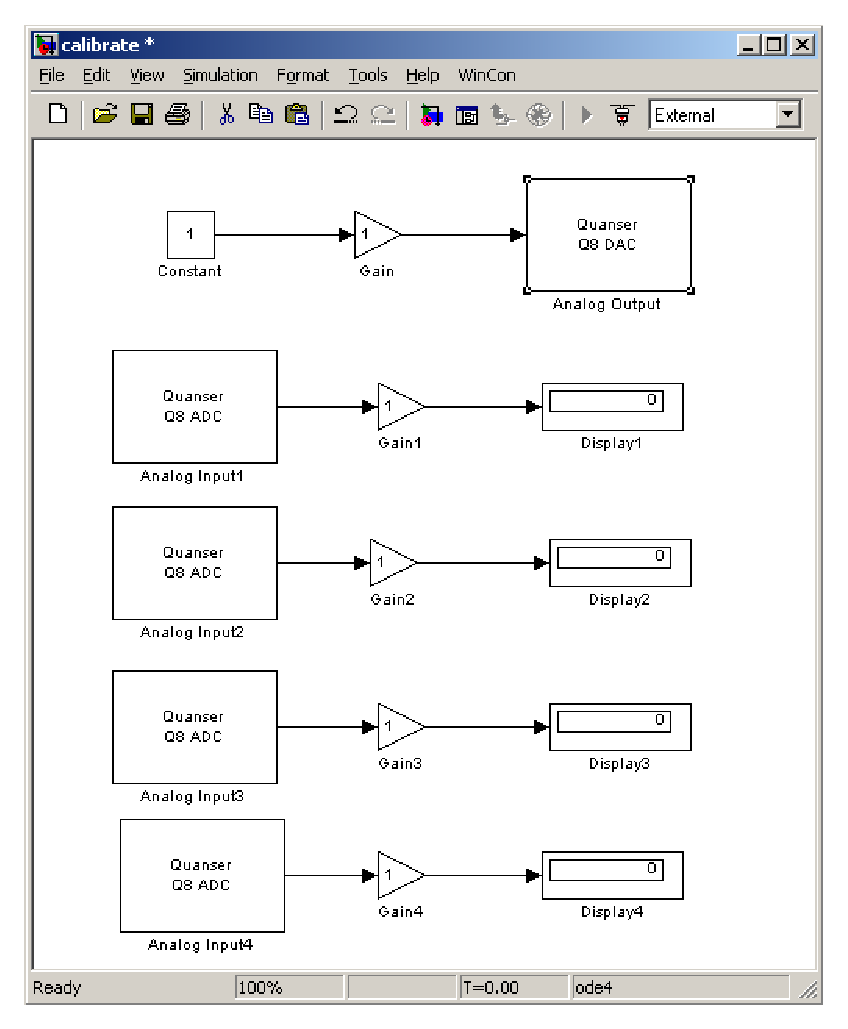
\includegraphics[width=.6\textwidth]{calibratemodel}
\caption{\footnotesize
        Simulink model for sensor calibration
        \label{fig.calibratemodel}
        }
\end{figure}

Next, add four analog input blocks (one for each of the RCA plugs on the DAQ board).  Connect them all to display blocks via unity gains.  Be sure to set their Channels to 1--4.  Now we are ready to build the code.
\par
\noindent\parbox{\textwidth}{
\mbox{\Large \textbf{Important}:}\\[3pt]
\indent \large Whenever you run an experiment that sends power to the motor, one team member must be assigned to operate the amplifier power switch.  Located on the back of the UPM, the ``kill switch'' is the only fail-safe method to cut power to the plant.\\[3pt]
\indent We do not know the internal gains associated with the plant and power module mechanisms.  How do we know that the constant ``1'' block will not overload the motor?  Mistakes \textit{do} happen, so to protect yourself, your teammates, and the equipment, always have someone ready to cut power in the event of an accident.
}

\vspace{6pt}

\par
In the WinCon Server, create four displays for the four sensor readings.  With a teammate on the kill switch, start the experiment.  Note that we have sent a positive constant voltage to the motor.  If the central gear rotates counterclockwise, then this is correct.  If it does not, change its gain to $-1$.
\par
Upon observing the four displays, you should see
\begin{itemize}
\item
    Two that hover around zero,
\item
    One that will remain relatively constant at a value other than zero, and
\item
    One that will revolve widely about zero.
\end{itemize}
From this, we know that the two channels that display zero data are not used.  We do not need to include them.  Further, the constant display is the tachometer; the revolving one corresponds to the potentiometer.
\par
Using a stopwatch, approximate the rotational speed of the central gear in revolutions per minute (rpm).  Using this measurement, change the gain block to accurately reflect the revolutions per minute (with the appropriate sign) of the system.
\par
Export the data from the potentiometer to MATLAB.  Find its minimum and maximum values.  From these, determine the calibration factor needed for the potentiometer to display in degrees.  Place this value in the potentiometer's gain block.  Also, add a scope on the potentiometer's output.
\par
After all this, your Simulink diagram should look something like Figure~\ref{fig.finalcalibrationmodel}.

\begin{figure}[bht]
\centering
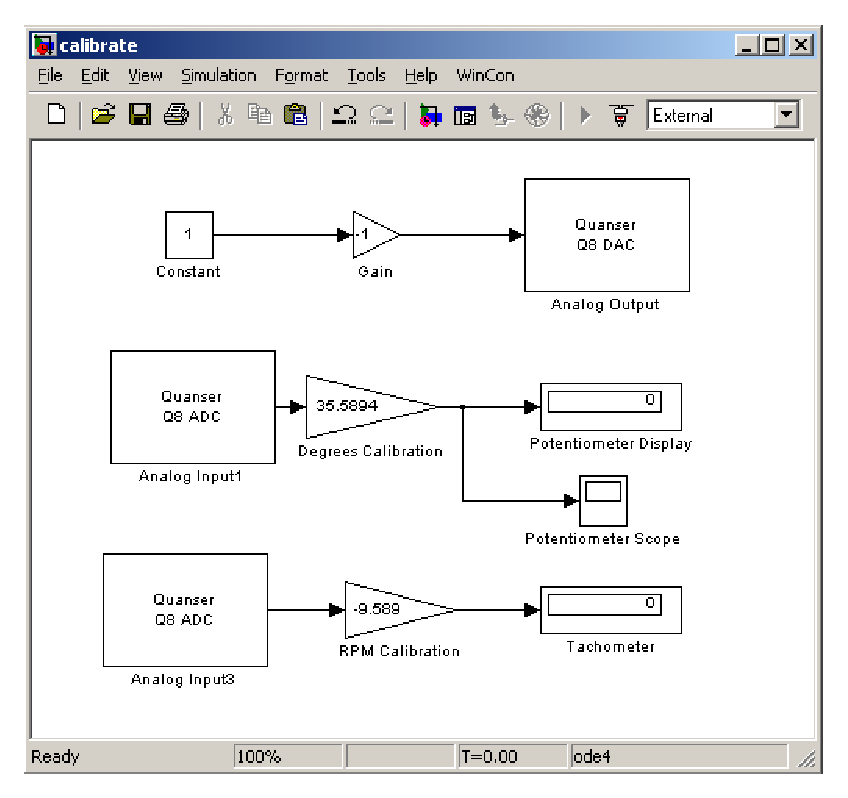
\includegraphics[width=.6\textwidth]{finalcalibrationmodel}
\caption{\footnotesize
        Example Simulink diagram with motor voltage sign inversion, tachometer calibration gain, and potentiometer calibration gain implemented.
        \label{fig.finalcalibrationmodel}
        }
\end{figure}

\par
For those interested, the potentiometer is a single-turn 10~k\textohm\ sensor with no physical stops.  Its electrical range is 352\textdegree.  The potentiometer generates an analog signal proportional to the angle of rotation.  The difference between a potentiometer and an encoder is that the encoder can measure several turns continuously while the potentiometer can only measure one full turn and then roll over.  Note that the potentiometer is an absolute position device while the encoder is a relative position device.  You can adjust the potentiometer shaft rotation relative to the gear such that the zero measurement is always at a desired angle.
\par
Create a well-labeled MATLAB plot of the calibrated potentiometer data over several periods of rotation.

% Lab 5:
% Op-Amp, A/D, D/A and Compensator Emulation

\chapter{A/D and D/A Converters and Compensator Emulation}
% Lab 6:
% Servo Position control design project:
% Position and Rate feedbacks

\newcommand{\circscale}{0.25}

\Opensolutionfile{PosConSolutions}
% \begin{solposcon}
% \end{solposcon}

\chapter[Servo Position Control: Position \& Rate Feedbacks]{Servo Position Control Design Project:\\ Position and Rate Feedbacks} \label{ch.PosCon}

Position control systems---also known as \textit{servomechanisms} or \textit{servos}---are used extensively in industrial applications such as robot9ics and drive control.  Modern position control systems are achieved using incremental encoder sensors.  In this project you design and implement a position control system for low frequency square wave input.  By the end of the project, you should have accomplished the following objectives:
\begin{itemize}
\item
    Obtain the servo plant model.
\item
    Design a position control systems such that the output angle tracks a commanded position using position and velocity feedback.  Also, determine the feedback gains to achieve the given time-domain specifications.
\item
    Build the compensated servo plant in Simulink and simulate offline to obtain the response to a square wave input to verify the design.
\item
    Build the WinCon application, implement, and test the system on real-time hardware.
\end{itemize}

\section{Pre-Lab Assignment}

Read the following introduction and perform the calculations required to simulate the control design.  Finishing these calculations before the laboratory session is critical to finishing on time.
\par
A position control system is one that converts a position input command to a position output response.  The first step in designing any control system is to generate a mathematical model of the physical system.  In this experiment, the familiar Quanser SRV-02 plant will be our servo.  A schematic of the servomotor is shown in Figure~\ref{fig.servomotorschematic}.  Many of the pertinent characteristics of the system are quantified in Table~\ref{tab.servoparams}

\begin{figure}[bht]
\centering
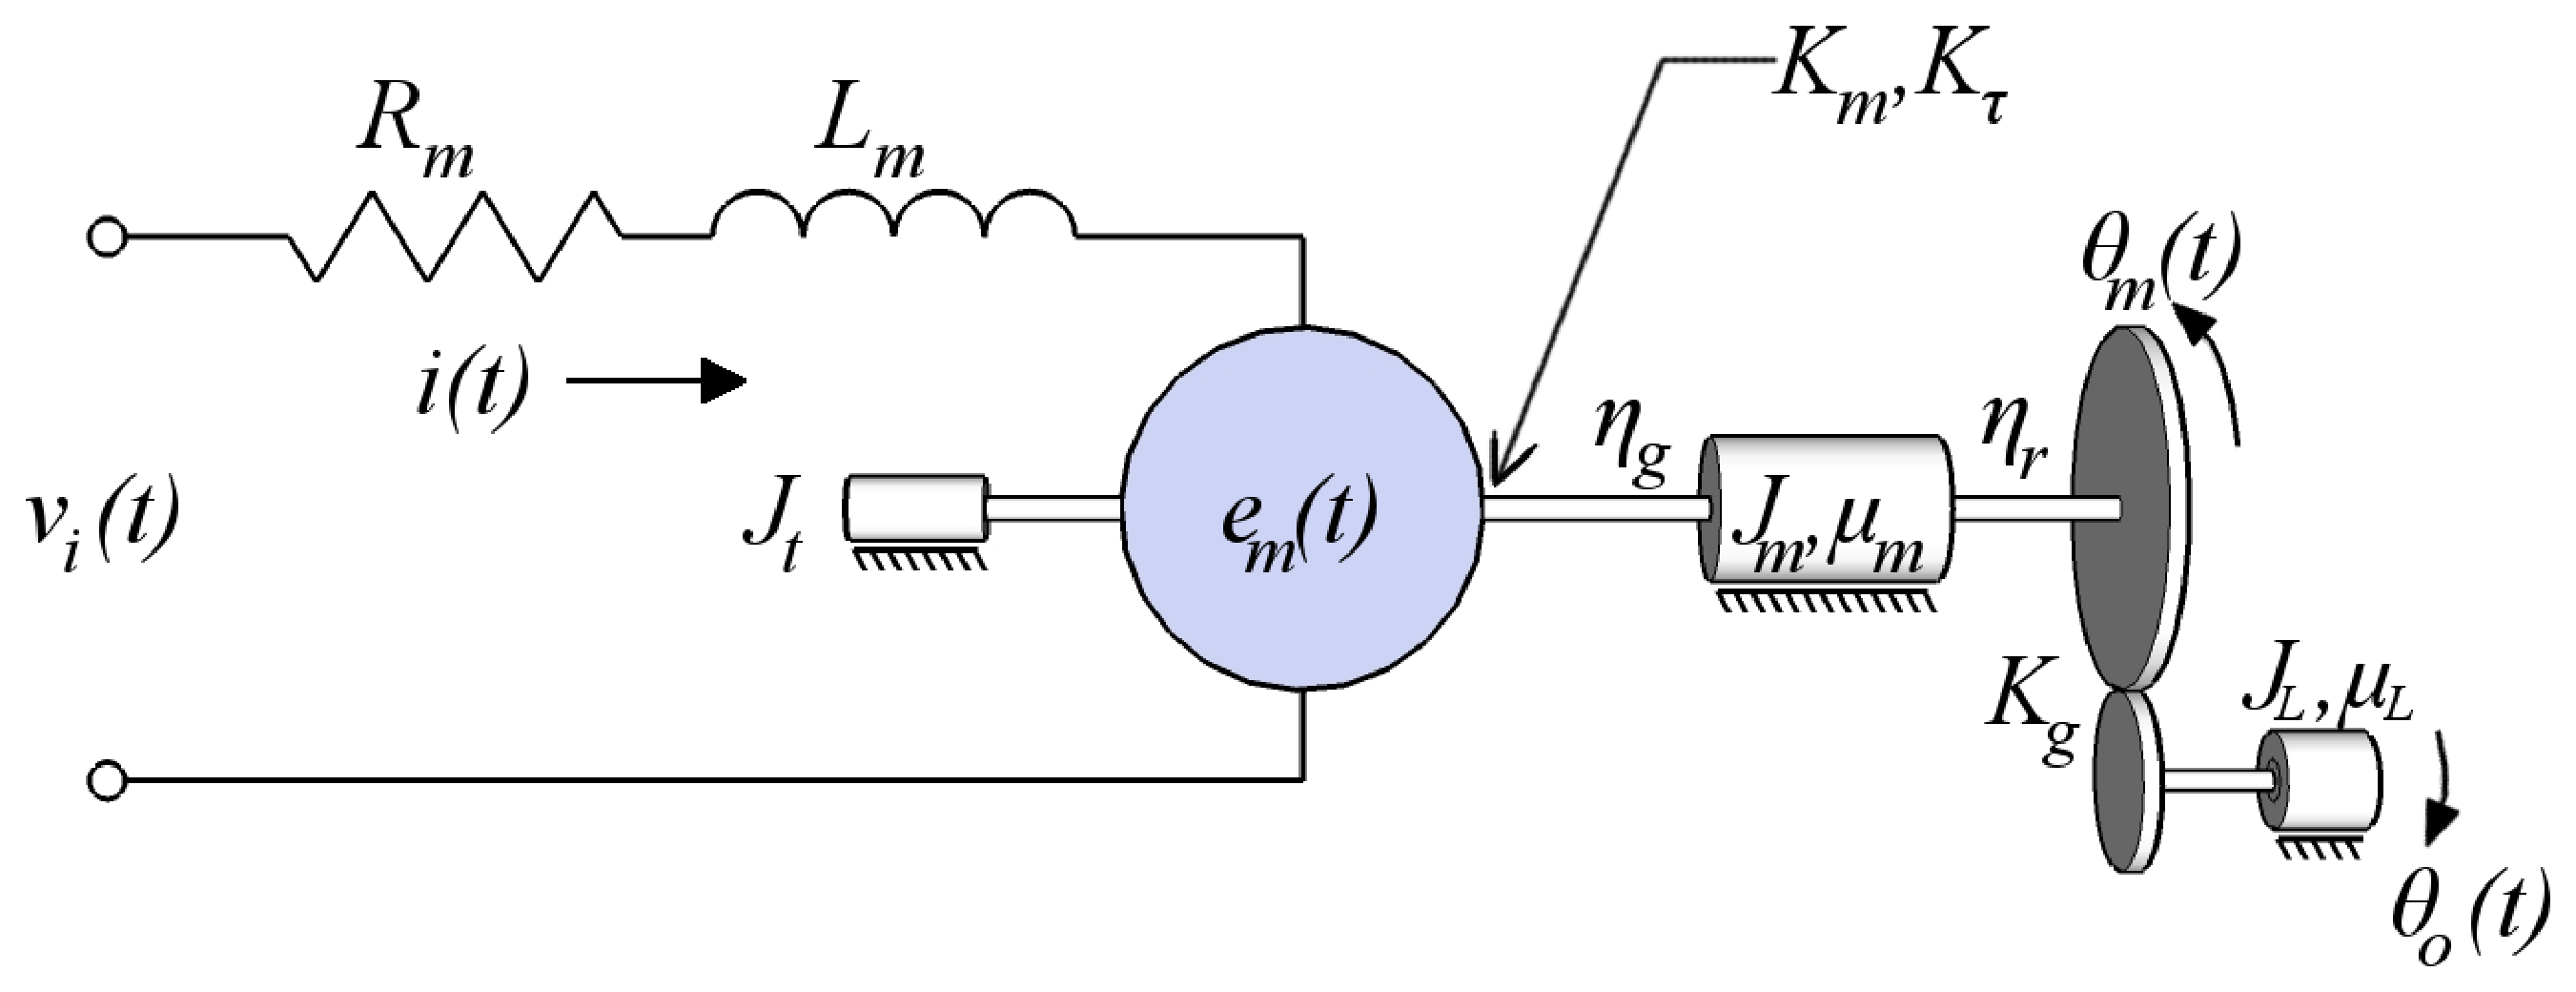
\includegraphics[scale=\circscale]{servomotor}
\caption{ \footnotesize
        Servo electromechanical schematic
        \label{fig.servomotorschematic}
        }
\end{figure}

\begin{table}[bht]
\centering \renewcommand{\arraystretch}{1.2}
\begin{tabular}{c | l | l}
    \textit{Symbol} &\multicolumn{1}{c|}{\textit{Parameter}} &
        \multicolumn{1}{c}{\textit{Value}} \\ \hline \hline
    $R_m$       &   Motor armature resistance   & $2.6\,\Omega$     \\
    $L_m$       &   Motor armature inductance   & $0.18\,$mH        \\
    $K_m$       &   Motor voltage constant      &$7.67\times10^{-3}\,$Vs/rad\\
    $K_\tau$    &   Motor torque constant       & $7.67\times10^{-3}\,$Nm/A \\
    $J_t$       &   Tachometer inertia          &
                                            $7\times10^{-8}\,\mbox{kg-m}^2$ \\
    $J_m$       &   Motor inertia       & $3.87\times10^{-7}\,\mbox{kg-m}^2$\\
    $\eta_g$    &   Gearbox efficiency          & $0.85$            \\
    $\eta_r$    &   Motor rotational efficiency & $0.87$            \\
    $K_g$       &   Transmission (gear) ratio   & $14$              \\
    $J_L$       &   Load inertia        & $1.6333\times10^{-5}\,\mbox{kg-m}^2$
\end{tabular}
\caption{\footnotesize
        Servo electric and mechanical characteristics
        \label{tab.servoparams}
        }
\end{table}
\par
Figure~\ref{fig.servomotorschematic} is a hybrid electric circuit diagram and mechanical schematic.  Looking at only the electric side, we see a fairly simply RL circuit with an input voltage $v_i(t)$ and voltage sink with emf $e_m(t)$.  In this sense, we can think of the electrical part of the servo as a subsystem (Figure~\ref{fig.servoelec}) and solve it in the frequency domain:
\begin{equation}
    I(s) = \frac{1}{R_m + L_m s} \left[V_i(s) - E_m(s)\right]
        \label{eq.servoelec}
\end{equation}
As is typical, capitalized forms of time variables represent their Laplace transforms.

\begin{figure}[bht]
\centering
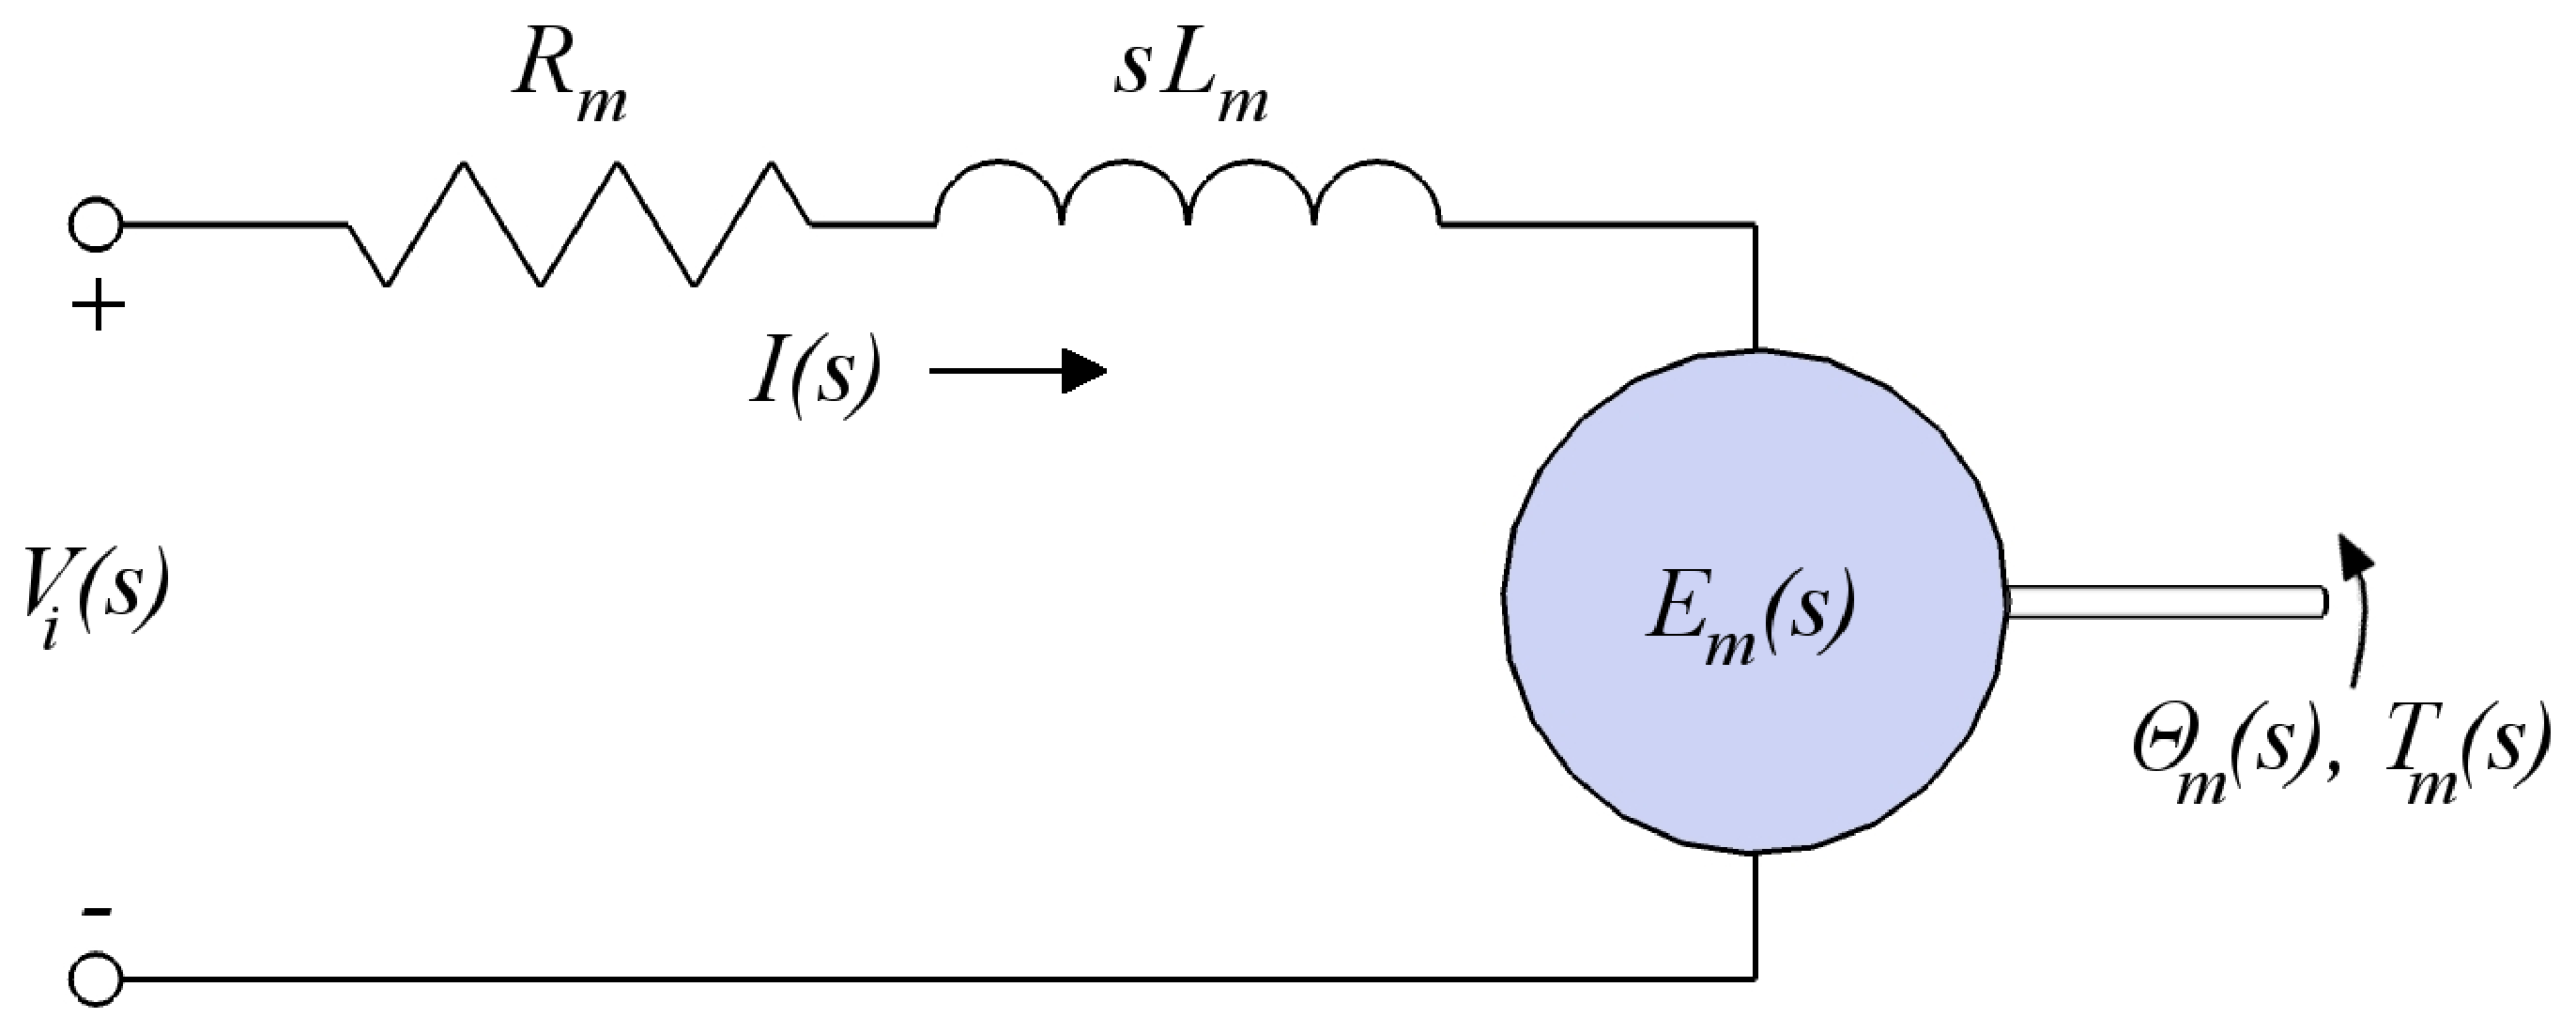
\includegraphics[scale=\circscale]{servoelec}
\caption{\footnotesize
        Servo electric circuit in the frequency domain
        \label{fig.servoelec}
        }
\end{figure}
\par
The torque produced by the motor, $\tau(t)$, is also proportional to the current, but we also must consider the losses due to gearbox inefficiency and rotational losses (like backlash).  Thus we model the motor's torque output as $\tau(t) = \eta_g \eta_r K_\tau i(t)$.  Which, in the frequency domain, is simply
\begin{equation}
    T(s) = \eta_g \eta_r K_\tau I(s)
\end{equation}
\par
The potential across the motor changes in time and is proportional to the angular velocity of the armature, $\dot{\theta}_m(t)$, and the change in the external magnetic field.  We will treat the ambient magnetic field as constant; we are left with the expression $e_m(t) = K_m \dot{\theta}_m(t)$.  Applying a Laplace transform and noting that differentiating in time is the same as multiplying by $s$ in frequency, we have:
\begin{equation}
    E_m(s) = K_m \Theta_m(s) s
\end{equation}
\par
Now that we have an expression for the output of the electric circuit in the servo---namely, the torque produced by the motor---we would like to move closer to our goal of solving for the motion of the output gear.  Again, we are looking for a closed-form expression that relates the voltage applied to the motor's circuit to the motion of the output gear (also known as the \textit{load} gear).
\par
As such, we transform the mechanical system of gears into an electric circuit analogy (see Lab~\ref{ch.ModSim} or \cite{analogs} for details on this conversion).  The analogous circuit is shown in Figure~\ref{fig.servoelecanalogy}.  For convenience, we have switched notation for the angular movement: $\dot{\theta} = \omega$ and $\mathcal{L}[\dot{\theta}] = \mathcal{L}[\omega] = \Omega(s) = s\Theta(s)$. There is a new element, however, in Fig.\ \ref{fig.servoelecanalogy}.  To represent the gear ratio between the motor and the load gears ($K_g$), we use the idea of an electrical transformer.  As an aside, the fundamental property of gears is that the ratio of parameters---including rotation speed, torque transmitted, number of teeth, and diameter---across gears is equal.  In our case, we have
\begin{equation*}
    K_g = \frac{\omega_m}{\omega_L} = \frac{T_1}{T_m} = \frac{N_L}{N_m} =
        \frac{d_L}{d_M}
\end{equation*}

\begin{figure}[bht]
\centering
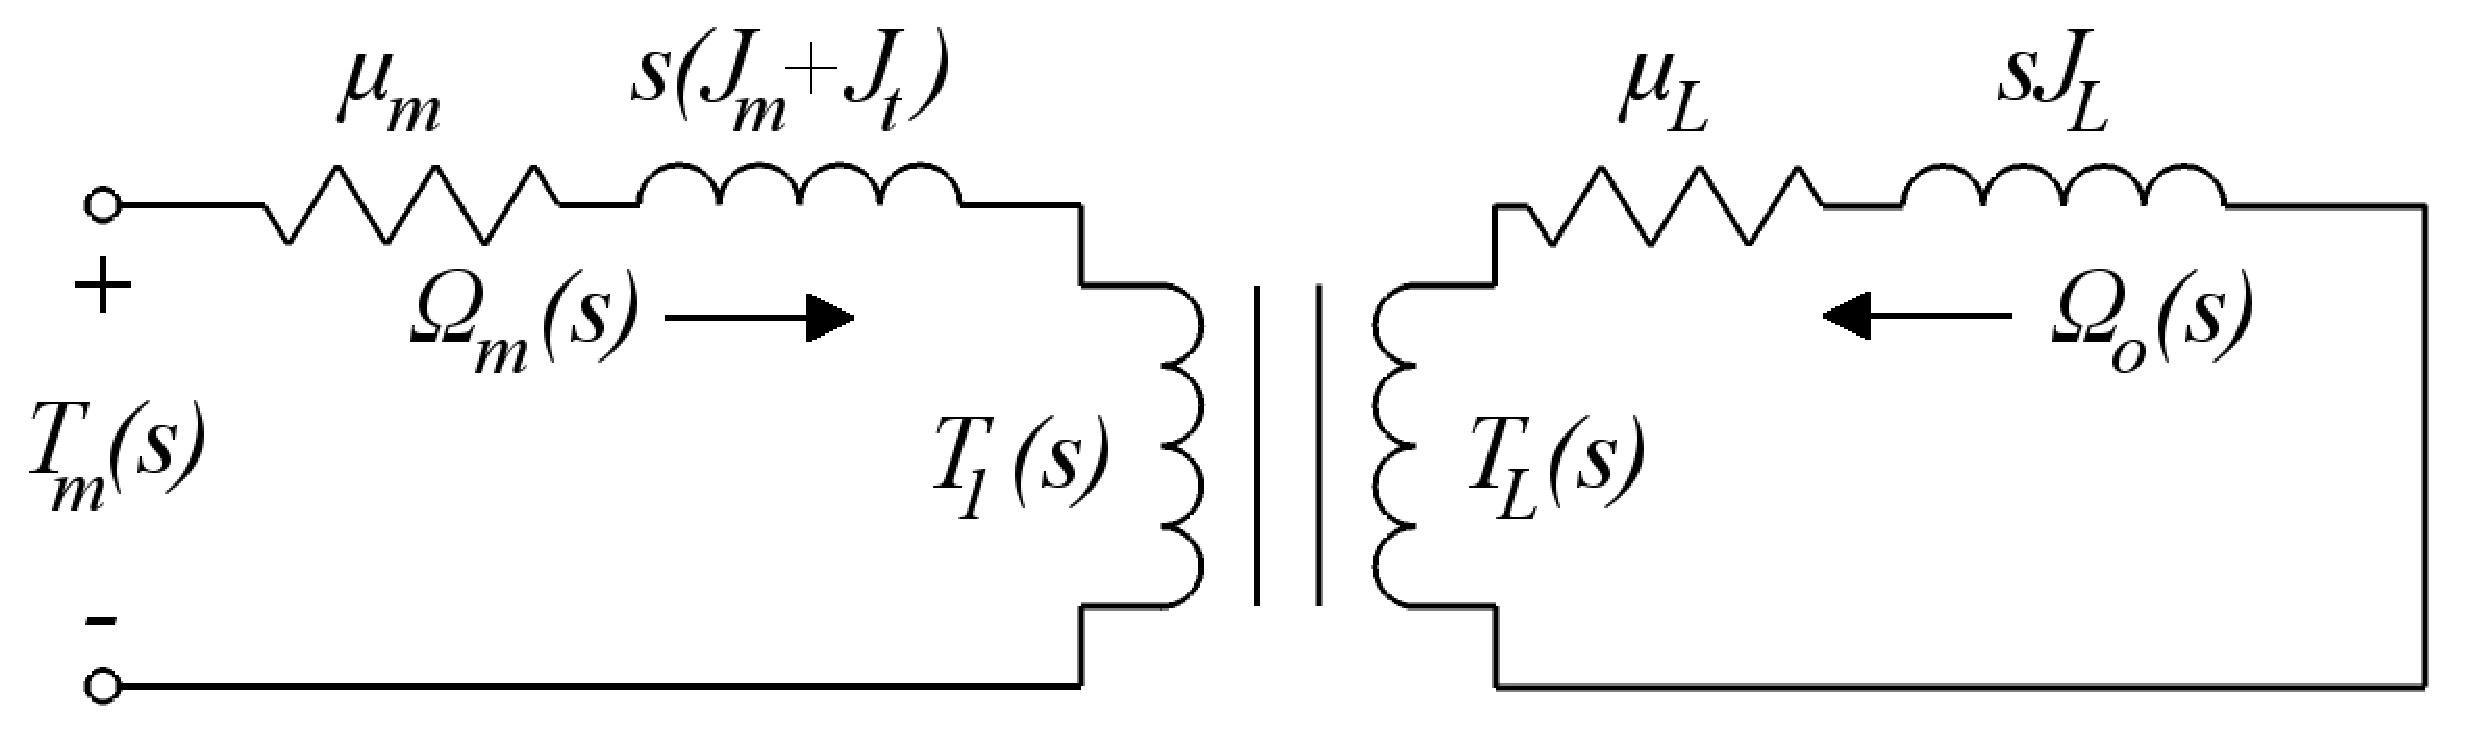
\includegraphics[scale=\circscale]{servoelecanalogy}
\caption{\footnotesize
        Electric circuit analogy for the mechanical part of the servo with quantities represented in the frequency domain.  The symbol at center is a transformer \cite{analogs}.
        \label{fig.servoelecanalogy}
        }
\end{figure}
\par
To aid in the modeling, we will now use a concept from mechanical systems to make an \textit{equivalent} system (see \cite{gears} for details).  Instead of dealing with two distinct axes of rotation (the motor shaft and the load gear shaft), we will speak instead as if all of the mechanisms were on the load shaft.  To ``move'' the motor and tachometer to the load shaft, we multiply the appropriate parameters by the square of the gear ratio and add.  Thus we get the equivalent friction and rotational inertias:
\begin{flalign*}
    \mu_{eq} &= K_g^2 \mu_m + \mu_L \approx 1\times10^{-3}\,\mbox{Nms/rad}\\
    J_{eq}   &= K_g^2(J_m + J_t) + J_L
\end{flalign*}
The equivalent system's circuit analog is shown in Figure~\ref{fig.servoelecequiv}.

\begin{figure}[bht]
\centering
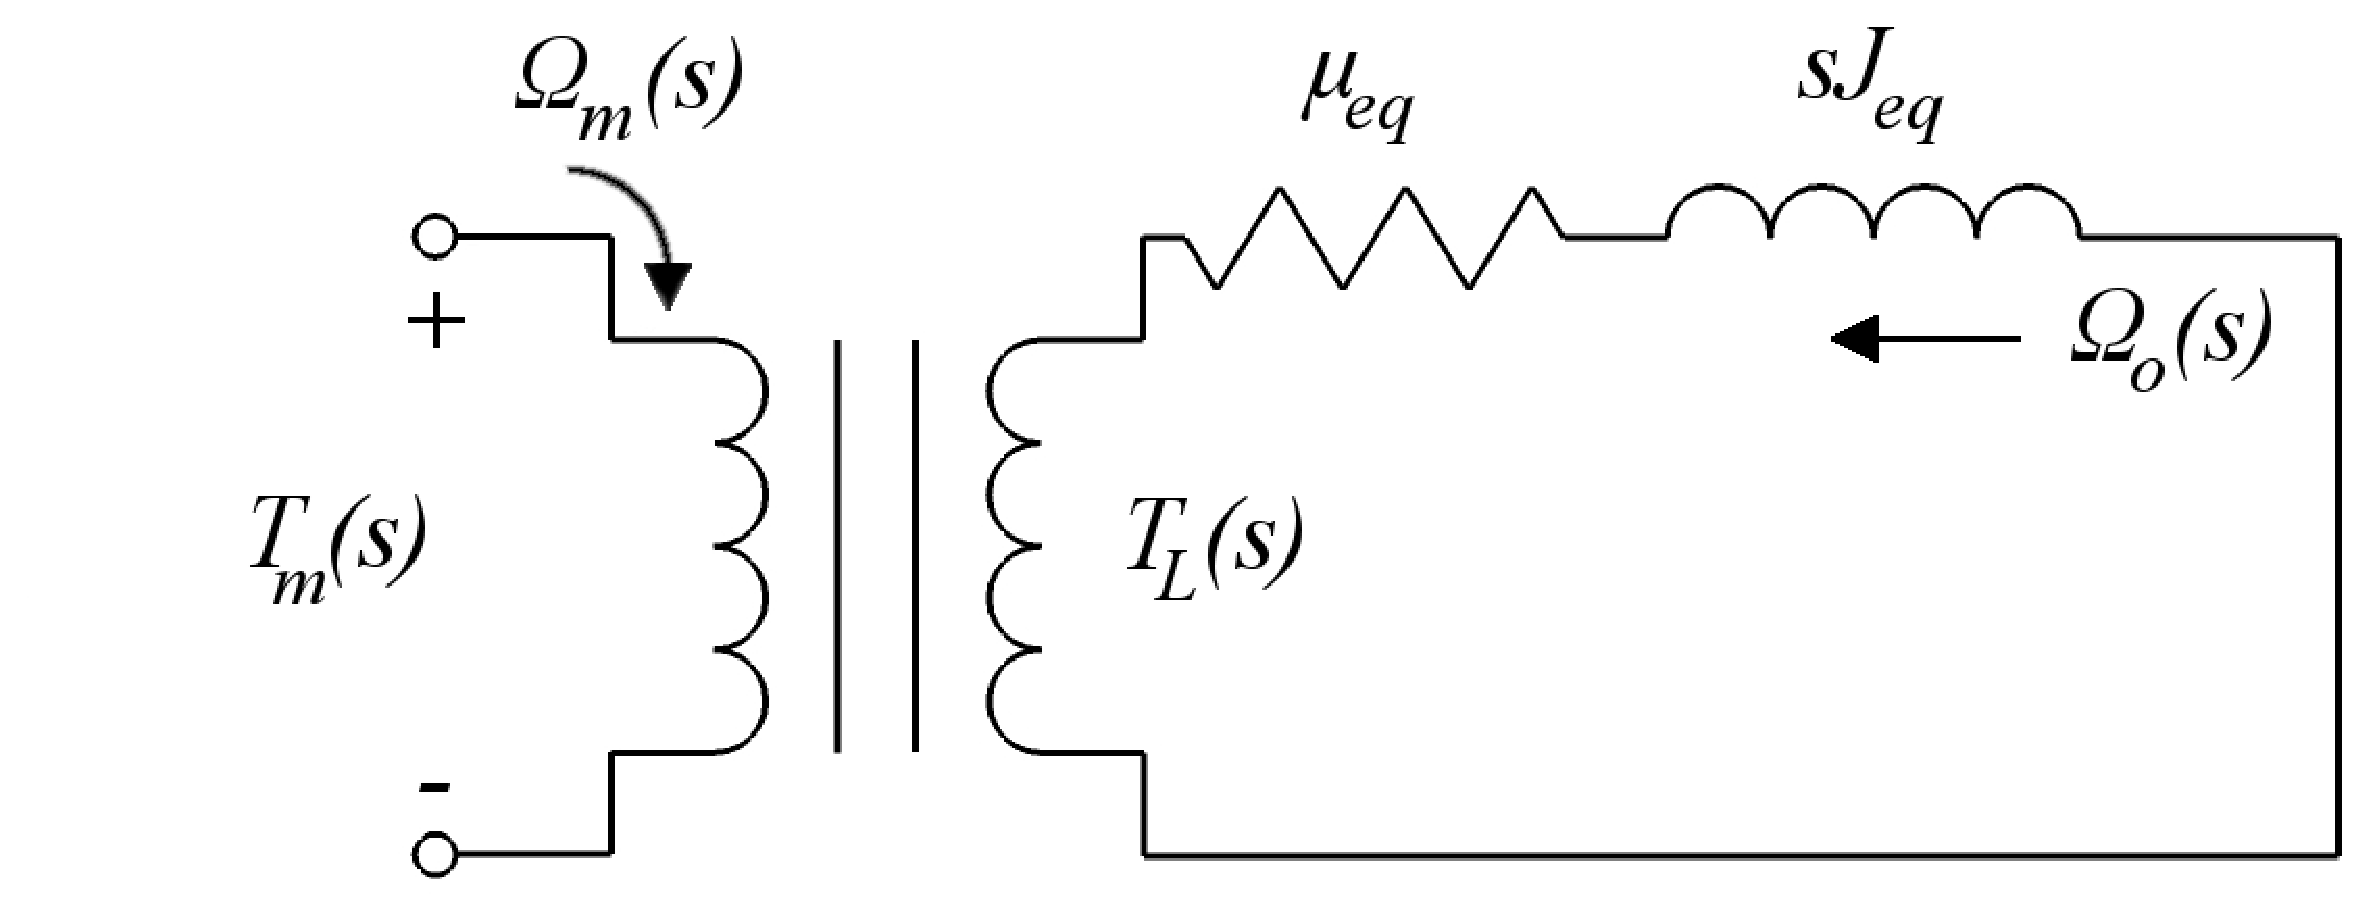
\includegraphics[scale=\circscale]{servoelecequiv}
\caption{\footnotesize
        Electric circuit analogy in the frequency domain for the equivalent mechanical system with all mechanical elements ``moved'' to the load shaft.
        \label{fig.servoelecequiv}
        }
\end{figure}
\par
From the circuit in Fig.\ \ref{fig.servoelecequiv} we have the following current relationships:
\begin{flalign}
    \Omega_o(s) & = \frac{1}{\mu_{eq} + sJ_{eq}} T_L(s) \\
    \frac{\Omega_m(s)}{\Omega_o(s)} & = K_g
        \label{eq.gearratiospeed}
\end{flalign}
\par
Using your knowledge of Laplace transforms and transfer functions, do the following:
\begin{enumerate}
\item
    Using Eqs.\ (\ref{eq.servoelec})--(\ref{eq.gearratiospeed}), draw a detailed block diagram representation for the servo system with $V_i(s)$ as input and $\Theta_o(s)$ as output.  Be sure to include all of the intermediate signals: $I(s)$, $E_m(s)$, $T_m(s)$, $T_L(s)$, and $\Omega_o(s)$.
        \begin{solposcon}
        The block diagram can be constructed by simply writing the pertinent equations one after the other and labeling the intermediate signals.  The full diagram should look something like Fig.\ \ref{fig.sol.poscon.blockdiagram}.
        \begin{figure}
        \centering
        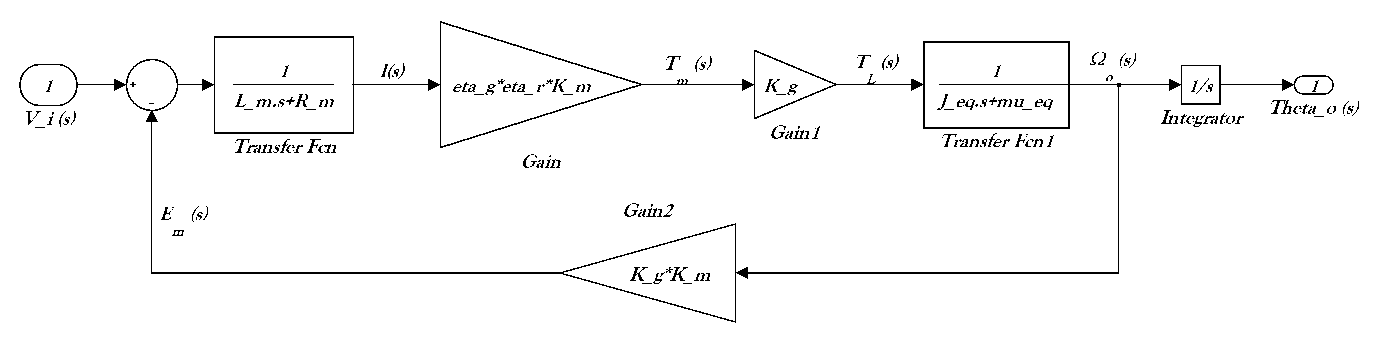
\includegraphics[angle=90, height=.95\textheight]{posconprelab1}
        \caption{\label{fig.sol.poscon.blockdiagram}}
        \end{figure}
        \end{solposcon}
\item
    We see that the motor electric time constant ($L_m/R_m$) is small compared to the mechanical time constants.  Thus, neglect the motor's electric inductance and obtain closed-loop transfer functions from $V_i(s)$ to $\Omega_o(s)$ and $\Theta_o(s)$.  You should obtain equations of the form
    \begin{flalign}
        \frac{\Omega_o(s)}{V_i(s)} &= \frac{a}{s+b} \mbox{ and } \\
        \frac{\Theta_o(s)}{V_i(s)} &= \frac{a}{s(s+b)}
    \end{flalign}
        \begin{solposcon}
        From the block diagram in question 1, it is a matter of reducing it to a single transfer function.  Use the rule that a negative feedback loop with block $G_1$ in the forward path and $G_2$ in the reverse path reduces to
        \begin{equation}
            G = \frac{G_1}{1+G_1G_2}
        \end{equation}
        After setting $L_m=0$, we have
        \begin{equation}
            TF_{V_i\to\Omega_o} =
                \frac{\frac{\eta K_m K_g}{R_m} \frac{1}{\mu_{eq} + J_{eq}s}}{ 1 + K_g K_m \frac{\eta K_m K_g}{R_m} \frac{1}{\mu_{eq} + J_{eq}s}}
        \end{equation}
        Note that $\eta := \eta_g \eta_r$.  To simplify, we multiply top and bottom of the big fraction by $\mu_{eq} + J_{eq}s$ to get
        \begin{equation}
            = \frac{
                    \frac{
                            \eta K_m K_g
                            }{
                            R_m
                            }
                    }{
                    \mu_{eq} + J_{eq}s + \frac{
                                                \eta K_m^2 K_g^2
                                                }{
                                                R_m
                                                }
                    }
        \end{equation}
        And now multiplying top and bottom by $1/J_{eq}$, we arrive at
        \begin{equation}
            = \frac{
                    \frac{
                            \eta K_m K_g
                            }{
                            R_m J_{eq}
                            }
                    }{
                    s + \frac{
                                \mu_{eq}
                                }{
                                J_{eq}
                                }
                    + \frac{
                            \eta K_m^2 K_g^2
                            }{
                            R_m J_{eq}
                            }
                    }
        \end{equation}
        Thus we have the correct form with pole-zero constants:
        \begin{subequations}
        \begin{gather}
            a = \frac{\eta K_m K_g}{R_m J_{eq}} \approx 288.3844\\
            b = \frac{\mu_{eq}}{J_{eq}} + \frac{\eta K_m^2 K_g^2}{R_m J_{eq}}
                \approx 40.4091
        \end{gather}
        \end{subequations}
        \par
        Finally, to get the TF to output position, we only need to pass the above TF through an integrator (it will have the same constants $a$ and $b$):
        \begin{equation}
            TF_{V_i\to\Theta_o} =
                \frac{a}{s(s+b)}
        \end{equation}
    \end{solposcon}
\item
    Use the Final Value Theorem to find the long-term position response to a unit step input.
        \begin{solposcon}
        The FVT looks like
        \begin{equation}
            \lim_{t\to\infty} \theta_o(t) = \lim_{s\to0}s\Theta_o(s)
        \end{equation}
        Applying this to our system, we have
        \begin{equation}
            \lim_{t\to\infty} \theta_o(t)
            =
            \lim_{s\to0} s \frac{1}{s} \frac{a}{s(s+b)} = \infty
        \end{equation}
        Some explanation:  The leading $s$ comes from the FVT itself.  The $1/s$ gives the systems response to a step input.  The rest of the expression is simply the transfer function to output position found in Question 2.
        \end{solposcon}
\item
    Now consider the servo system as a control system.  Until now, we have only had the voltage $v_i$ as the input and we simply observed its effect on the output position.  Now let us have a certain angle (position) be the input. We will obviously need some sort of conversion to turn this \textit{command} into a voltage that we can send the motor.  Call this conversion a gain and label it $K_P$.  Now the block diagram for the system looks something like Figure~\ref{fig.servoKp}.
    \begin{figure}[hbt]
    \centering
    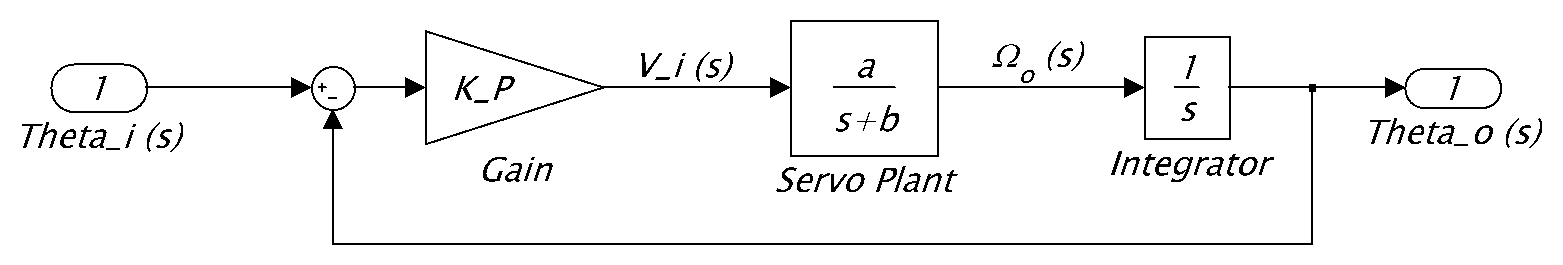
\includegraphics[width=.9\textwidth]{posconprelabKP}
    \caption{\footnotesize
            Position control block diagram with position feedback
            \label{fig.servoKp}
            }
    \end{figure}
    We call the scheme pictured in Fig.\ \ref{fig.servoKp} \textit{proportional control}.  We are able to scale the tracking error by adjusting the gain $K_P$ that gauges the voltage applied to the servo. \\
    Additionally, we can feed back the velocity signal to improve our control system's performance.  We will also run it through a gain called $K_D$.  Now the system looks like Figure~\ref{fig.servoPD}.
    \begin{figure}[bht]
    \centering
    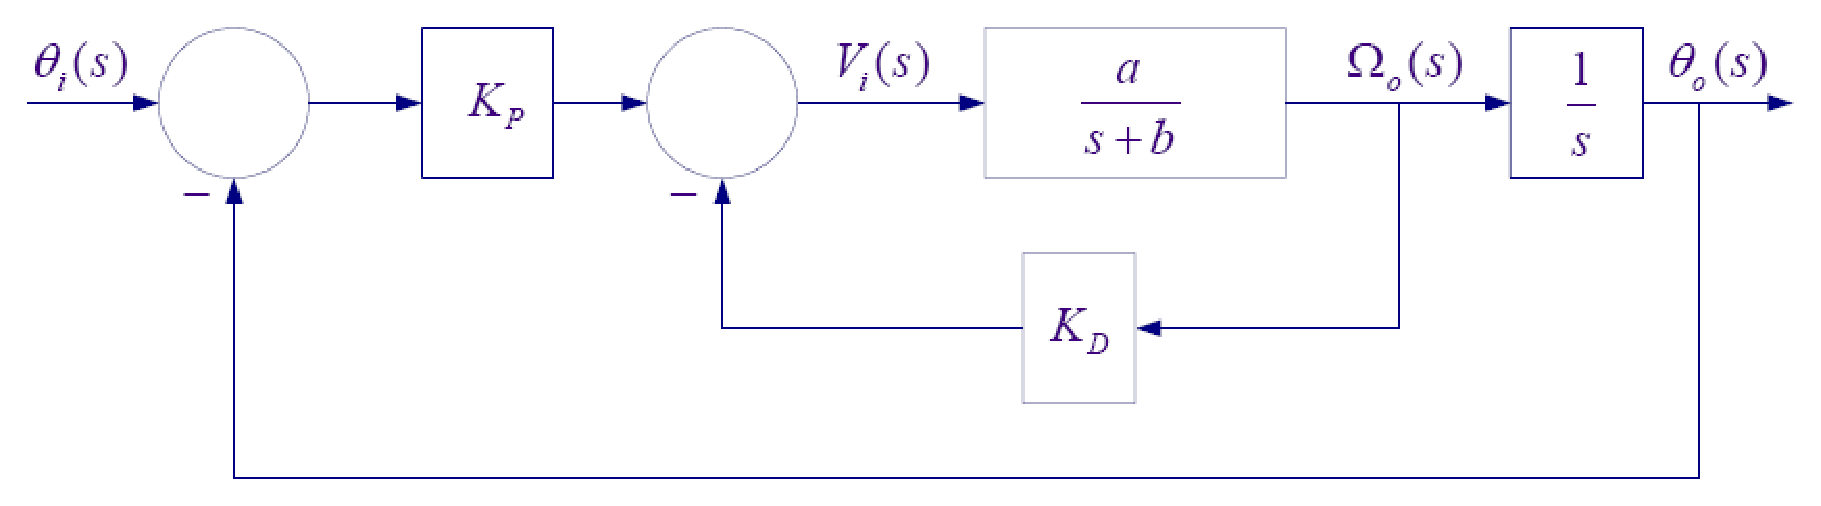
\includegraphics[width=.9\textwidth]{posconprelabPDblock}
    \caption{\footnotesize
            Position control block diagram with position and rate feedbacks (PD control).
            \label{fig.servoPD}
            }
    \end{figure}
    Find the transfer function from $\theta_i(s)$ to $\theta_o(s)$ in Figure~\ref{fig.servoPD}.
        \begin{solposcon}
        The inner feedback loop (the derivative control) in Fig.\ \ref{fig.servoPD} can be reduced to
        \begin{equation}
            G_1(s) := \frac{
                            \frac{a}{s+b}
                            }{
                            1+K_D\frac{a}{s+b}
                            }
        \end{equation}
        Then in the forward path of the remaining diagram, we have $K_P G_1(s)/s$.  The remaining diagram is a simple unity feedback system:
        \begin{equation}
            TF_{\Theta_i\to\Theta_o} :=
            \frac{K_P G_1(s)/s}{1+K_P G_1(s)/s}
                \label{eq.servoPDtf}
        \end{equation}
        Simplifying Equation~(\ref{eq.servoPDtf}) yields the classical second-order transfer function:
        \begin{equation}
            TF_{\Theta_i\to\Theta_o} =
            \frac{
                K_P a
                }{
                s^2 + s(b+K_D a) + K_P a
                }
                \label{eq.servoPD}
        \end{equation}
        \end{solposcon}
\item
    Let $\theta_i(t)$ be a square wave with amplitude 20\textdegree\ and a frequency of $1\,\mbox{Hz}$.  Determine the values for the gains $K_P$ and $K_D$ in Fig.\ \ref{fig.servoPD} such that the following time-domain specifications are met:
    \begin{itemize}
    \item A damping ratio, $\zeta = 0.707$
    \item A peak time of $t_p = 0.05\,\mbox{seconds}$.
    \end{itemize}
    For your reference, the peak time of a second-order system is given by
    \begin{equation}
        t_p = \frac{\pi}{\omega_n \sqrt{1-\zeta^2}}
    \end{equation}
    and the theoretical peak value of the response to a step input is
    \begin{equation}
        M_p = \left(1 + e^{\frac{
                                -\zeta \pi
                                }{
                                \sqrt{1-\zeta^2}
                                }
                                }
                \right) \max \theta_i
    \end{equation}
    Note that the servo's PD transfer function has the same form as the standard second-order transfer function:
    \begin{equation}
        \frac{\Theta_o(s)}{\Theta_i(s)}
        =
        \frac{
                K\omega_n^2
                }{
                s^2 + 2\zeta\omega_n s + K\omega_n^2
                }
            \label{eq.secondordertf}
    \end{equation}
        \begin{solposcon}
        Comparing Eqs.\ (\ref{eq.secondordertf}) and (\ref{eq.servoPD}), we can conclude the following basic parameters:
        \begin{subequations}
        \begin{flalign}
        K &= 1 \\
        \omega_n &= \sqrt{K_P a} \\
        \zeta &= \frac{b+K_D a}{2\sqrt{K_P a}} \label{eq.servoDR}
        \end{flalign}
        \end{subequations}
        We then translate the formula given for peak time into one with our parameters:
        \begin{equation}
        t_p =  \frac{\pi}{\omega_n \sqrt{1-\zeta^2}}
        = \frac{
                \pi
                }{
                \sqrt{K_P a}\sqrt{1-\frac{
                                        (b+K_D a)^2
                                        }{
                                        4K_P a
                                        }
                                        }
                }
            \label{eq.servoPT}
        \end{equation}
        Now we have a system of equations with two unknowns ($K_P$, and $K_D$) and two equations (\ref{eq.servoDR} and \ref{eq.servoPT}).  You can solve these using your favorite method.  One way would be to rearrange Eq.\ \ref{eq.servoDR} for $K_D$ and then substitute into Eq.\ \ref{eq.servoPT} to solve for $K_P$ first.  Using $K_P$, you can then go back and find $K_D$.
        \par
        These parameters turn out to be:
        \begin{flalign*}
            K_P &\approx 27.3708 \\
            K_D &\approx 0.2955
        \end{flalign*}
        \end{solposcon}
\item
    Create a Simulink model of the PD control system we have just derived.  Use the values for $a$, $b$, $K_P$, and $K_D$ from above.  The Simulink model should look similar to Figure~\ref{fig.servoPDmodel}.  Change the simulation parameters to a``Fixed-step'' of 0.001 and ``ode4 (Runge-Kutta).''
    \begin{figure}[bht]
    \centering
    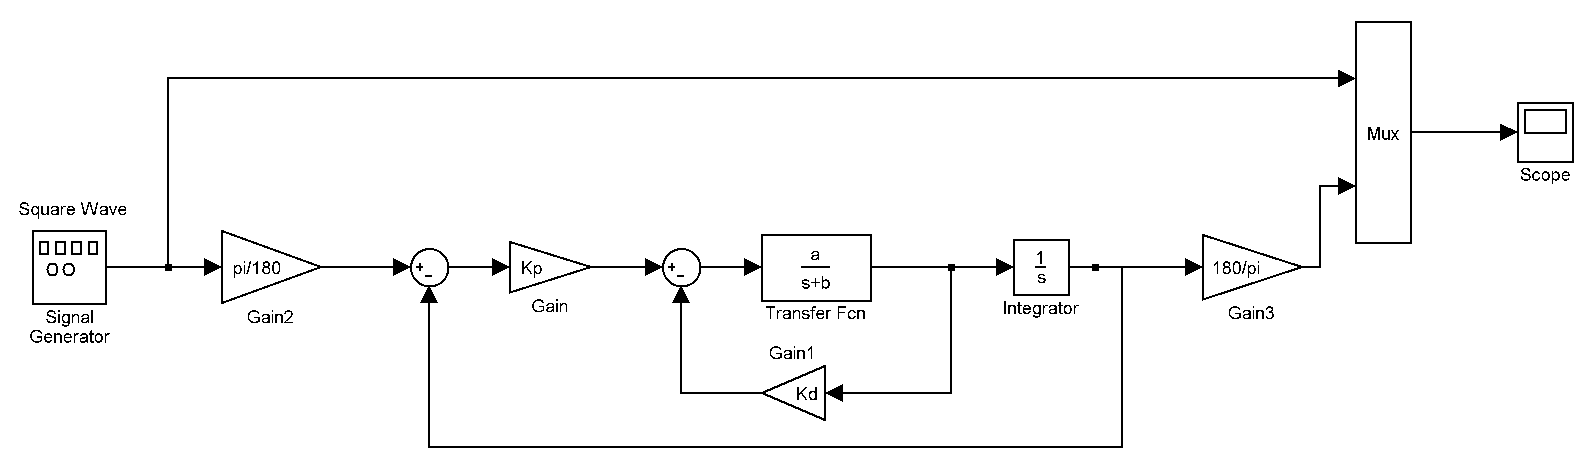
\includegraphics[width=.9\textwidth]{posconprelabPD}
    \caption{\footnotesize
            Simulink model for servo position PD control
            \label{fig.servoPDmodel}
            }
    \end{figure}
    Simulate and use the \verb=plotscope= function to capture the scope's plot and put it in a MATLAB figure plot.  Check to see if the response meets the design requirements.
        \begin{solposcon}
        The solution to this question is provided in Fig.\ \ref{fig.servoPDmodel}.
        \end{solposcon}
\end{enumerate}

All of the prelab calculations, design, and simulation must be completed prior to the laboratory session.  The plant transfer function and controller values must be checked and verified by the instructor prior to implementation.

\begin{thebibliography}{9}
    \bibitem{ogata} Katsuhiko Ogata.  Modern Control Engineering, 4th edition.  Prentice Hall.  2002.
    \bibitem{gears} Giancarlo Genta.  Dynamics of Rotating Systems.  Springer.  2005.
    \bibitem{analogs} Eric Cheever.  Electrical and Mechanical Analogs. \url{http://www.swarthmore.edu/NatSci/echeeve1/Ref/Analogs/ElectricalMechanicalAnalogs.html}
\end{thebibliography}

\Closesolutionfile{PosConSolutions}
% Lab 7:
% Speed control design project:
% Velocity feedback
% Lab 8:
% Position Control design project:
% PD Controller---root locus design
% Lab 9:
% Position Control Design project
% Phase lead controller---root locus design
% Lab 10:
% Ball and Beam Design project
\appendix
\include{AppMAT}
% APPENDIX
% State Space Intro
\chapter{Basics of State Space Modeling} \label{app.statespace}
\section{Introductory Concepts}

The differential equations of a lumped linear network can be written in the form
\begin{subequations}
\begin{flalign}
    \dot{\vec{x}}(t)    & = A\vec{x}(t) + B\vec{u}(t) \label{eq.stateeq}\\
    \vec{y}(t)    & = C\vec{x}(t) + D\vec{u}(t) \label{eq.outputeq}
\end{flalign}
\end{subequations}
Equation~(\ref{eq.stateeq}) is a system of first-order differential equations and is known as the \uline{state equation} of the system.  The vector $\vec{x}(t)$ is the \uline{state} vector, and $\vec{u}(t)$ is the \uline{input} vector.  Equation~(\ref{eq.outputeq}) is referred to as the \uline{output equation}.  $A$ is called the state matrix, $B$ the input matrix, $C$ the output matrix, and $D$ is the direct transition matrix.
\par
One advantage of the state space method is that the form lends itself easily to the digital and analog computation methods of solution.  Further, the state space method can be easily extended to the analysis of nonlinear systems.
\par
State equations may be obtained from an $n^{th}$ order differential equation or directly from the system model by identifying appropriate state variables.  To illustrate the first method, consider an $n^{th}$ order linear plant model described by the differential equation
\begin{equation}
    \frac{d^ny}{dt^n} + a_{n-1} \frac{d^{n-1}y}{dt^{n-1}} +
        \cdots + a_1 \frac{dy}{dt} + a_0 y = u(t)
        \label{eq.nthorder}
\end{equation}
Where $y(t)$ is the plant output and $u(t)$ is the plant input.  A state model for this system is not unique but depends on the choice of a set of state variables.  A useful set of state variables, referred to as \uline{phase variables}, is defined as:
\begin{equation}
    x_1 = y, \quad x_2 = \dot{y}, \quad x_3 = \ddot{y}, \ldots,
        x_n = \frac{d^{n-1}y}{dt^{n-1}}
        \label{eq.differentiatestate}
\end{equation}
\par
Taking derivatives of the first $n-1$ state variables, we have
\begin{equation}
    \dot{x}_1 = x_2, \quad \dot{x}_2 = x_3, \quad
        \ldots, \quad \dot{x}_{n-1} = x_n
    \label{eq.dotstatechain}
\end{equation}
In addition, $\dot{x}_n$ comes from rearranging Eq.~(\ref{eq.nthorder}) and substituting from Eq.~(\ref{eq.differentiatestate}):
\begin{equation}
    \dot{x}_n = -a_0x_1 - a_1x_2 -\cdots-a_{n-1}x_n + u(t)
    \label{eq.dotstatesub}
\end{equation}
In matrix form, this looks like
\begin{equation}
    \left[ \begin{array}{c} \dot{x}_1 \\ \dot{x}_2 \\ \vdots \\
                    \dot{x}_{n-1} \\ \dot{x}_n \end{array} \right]
    =
    \left[ \begin{array}{ccccc}
            0   &   1   &   0   &   \cdots  &   0   \\
            0   &   0   &   1   &   \cdots  &   0   \\
            \vdots&\vdots&\vdots&   \ddots  & \vdots\\
            0   &   0   &   0   &   \cdots  &   1   \\
            -a_0&   -a_1&   -a_2&   \cdots  &   -a_{n-1}
            \end{array} \right]
    \left[ \begin{array}{c} x_1 \\ x_2 \\ \vdots \\
                    x_{n-1} \\ x_n \end{array} \right]
    +
    \left[ \begin{array}{c} 0 \\ 0 \\ \vdots \\
                    0 \\ 1 \end{array} \right] u(t)
\end{equation}
Thus the output equation is simply
\begin{equation}
    y = \left[ \begin{array}{ccccc}1&0&0&\cdots&0\end{array} \right] \vec{x}
\end{equation}
\par
\begin{workex} \label{ex.phasevarstatespace}
Obtain the state equation in phase variable form for the following differential equation:
\begin{equation*}
    2\frac{d^3y}{dt^3} + 4\frac{d^2y}{dt^2} + 6\frac{dy}{dt} + 8y = 10u(t)
\end{equation*}
\textit{Solution}:
\par
The differential equation is third order, and thus there are three state variables: $x_1 = y$, $x_2 = \dot{y}$, and $x_3 = \ddot{y}$.  The first derivatives are:
\begin{flalign*}
    \dot{x}_1 & = x_2 \\
    \dot{x}_2 & = x_3 \\
    \dot{x}_3 & = -4x_1 - 3x_2 - 2x_3 + 5u(t)
\end{flalign*}
Or, in matrix form:
\begin{flalign*}
    \left[ \begin{array}{c} \dot{x}_1 \\ \dot{x}_2 \\ \dot{x}_3 \end{array}
        \right]
    & =
    \left[ \begin{array}{rrr}0&1&0\\0&0&1\\-4&-3&-2\end{array} \right]
    \left[ \begin{array}{c} x_1 \\ x_2 \\ x_3 \end{array} \right]
    +
    \left[ \begin{array}{c} 0\\0\\5 \end{array}\right] u(t)
    \\
    y & =
    \left[ \begin{array}{ccc}1&0&0\end{array}\right]
    \left[ \begin{array}{c} x_1 \\ x_2 \\ x_3 \end{array} \right]
\end{flalign*}
\end{workex}
\par
The m-file \verb=ode2phv.m= was developed to convert an $n^{th}$ order ordinary differential equation to the state space phase variable form.  The syntax is \verb#[A, B, C] = ode2phv(ai,k)#, and returns the typical three matrices.  The input \verb=ai= is a row vector containing the coefficients of the equation in descending order, and \verb=k= is the coefficient on the right hand side.  Using the ODE from Example \ref{ex.phasevarstatespace}, we would enter:

\begin{codex}
>> ai = [2 4 6 8];
>> k = 10;
>> [A, B, C] = ode2phv(ai,k)
A =
    0   1   0
    0   0   1
    -4  -3  -2
B =
    0
    0
    5
C =
    1   0   0
>>
\end{codex}

\subsubsection{Equations of Electrical Networks}
The state variables are directly related to the energy storage elements of a system.  It would seem, therefore, that the number of independent initial conditions is equal to the  number of energy storing elements.  This is true---provided that there is no loop containing only capacitors and voltage sources, and there is no cut set containing only inductive and current sources. In general, if there are $n_C$ loops of all capacitors and voltages sources, and $n_L$ cut sets of all inductors and current sources, the number of state variables is
\begin{equation}
    n = e_L + e_C - n_C - n_L
\end{equation}
where $e_L$ and $e_C$ are the numbers of inductors and capacitors, respectively.

\begin{figure}[bth]
\centering
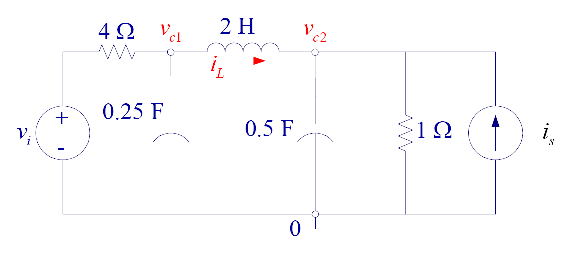
\includegraphics[width=.6\textwidth]{statespaceelecnet}
\caption{\footnotesize
        Circuit of Example~\ref{ex.elecnet}
        \label{fig.statespace.elecnet}
        }
\end{figure}

\begin{workex} \label{ex.elecnet}
Write the state equation for the network shown in Figure~\ref{fig.statespace.elecnet}.\\
\textit{Solution}:
\par
Define the state variables as current through the inductor and voltage across the capacitors.  Write two node equations containing capacitors and a loop equation containing the inductor.  The state variables will be $v_{c1}$, $v_{c2}$, and $i_L$.
\par
Node equations:
\begin{flalign*}
    0.25\frac{dv_{c1}}{dt} + i_L + \frac{v_{c1}-v_i}{4} = 0 & \Rightarrow
        \dot{v}_{c1} = -v_{c1} - 4i_L + v_i \\
    0.5 \frac{dv_{c2}}{dt} - i_L + v_{c2} - i_s = 0 & \Rightarrow
        \dot{v}_{c2} =  -2i_L +2 v_{c2} + 2i_s
\end{flalign*}
Loop equation:
\begin{flalign*}
    2\frac{di_L}{dt} + v_{c2} -v_{c1} = 0 & \Rightarrow
        \dot{i}_L = 0.5v_{c1} -0.5v_{c2}
\end{flalign*}
\par
Equivalently, in matrix form:
\begin{equation*}
    \left[ \begin{array}{c} \dot{v}_{c1} \\ \dot{v}_{c2} \\ \dot{i}_L
        \end{array} \right]
    =
    \left[ \begin{array}{rrr} -1&0&-4\\0&-2&2\\0.5&-0.5&0 \end{array}
        \right]
    \left[ \begin{array}{c} v_{c1} \\ v_{c2} \\ i_L
        \end{array} \right]
    +
    \left[ \begin{array}{cc} 1&0\\0&2\\0&0 \end{array}\right]
    \left[ \begin{array}{c} v_i \\ i_s \end{array} \right]
\end{equation*}
\end{workex}

\subsection{Simulation Diagrams}

Equations~(\ref{eq.dotstatechain}) and (\ref{eq.dotstatesub}) indicate that state variables are determined by integrating the corresponding state equation.  A diagram known as the \uline{simulation diagram} can be constructed to model the given differential equations.  The basic element of the simulation diagram is the integrator.  The first equation in (\ref{eq.dotstatechain}) is $\dot{x}_1  = x_2$.  Integrating we have:
\begin{equation*}
    x_1 = \int x_2 dx
\end{equation*}
\par
The above integral is represented by the time-domain block diagram shown in Figure~\ref{fig.statespace.inttimedom} and by the signal flow graph in Figure~\ref{fig.statespace.intsigflow}.

\newsavebox{\tempbig}
\newsavebox{\tempsmall}
\begin{figure}[bht]
\centering
\sbox{\tempbig}{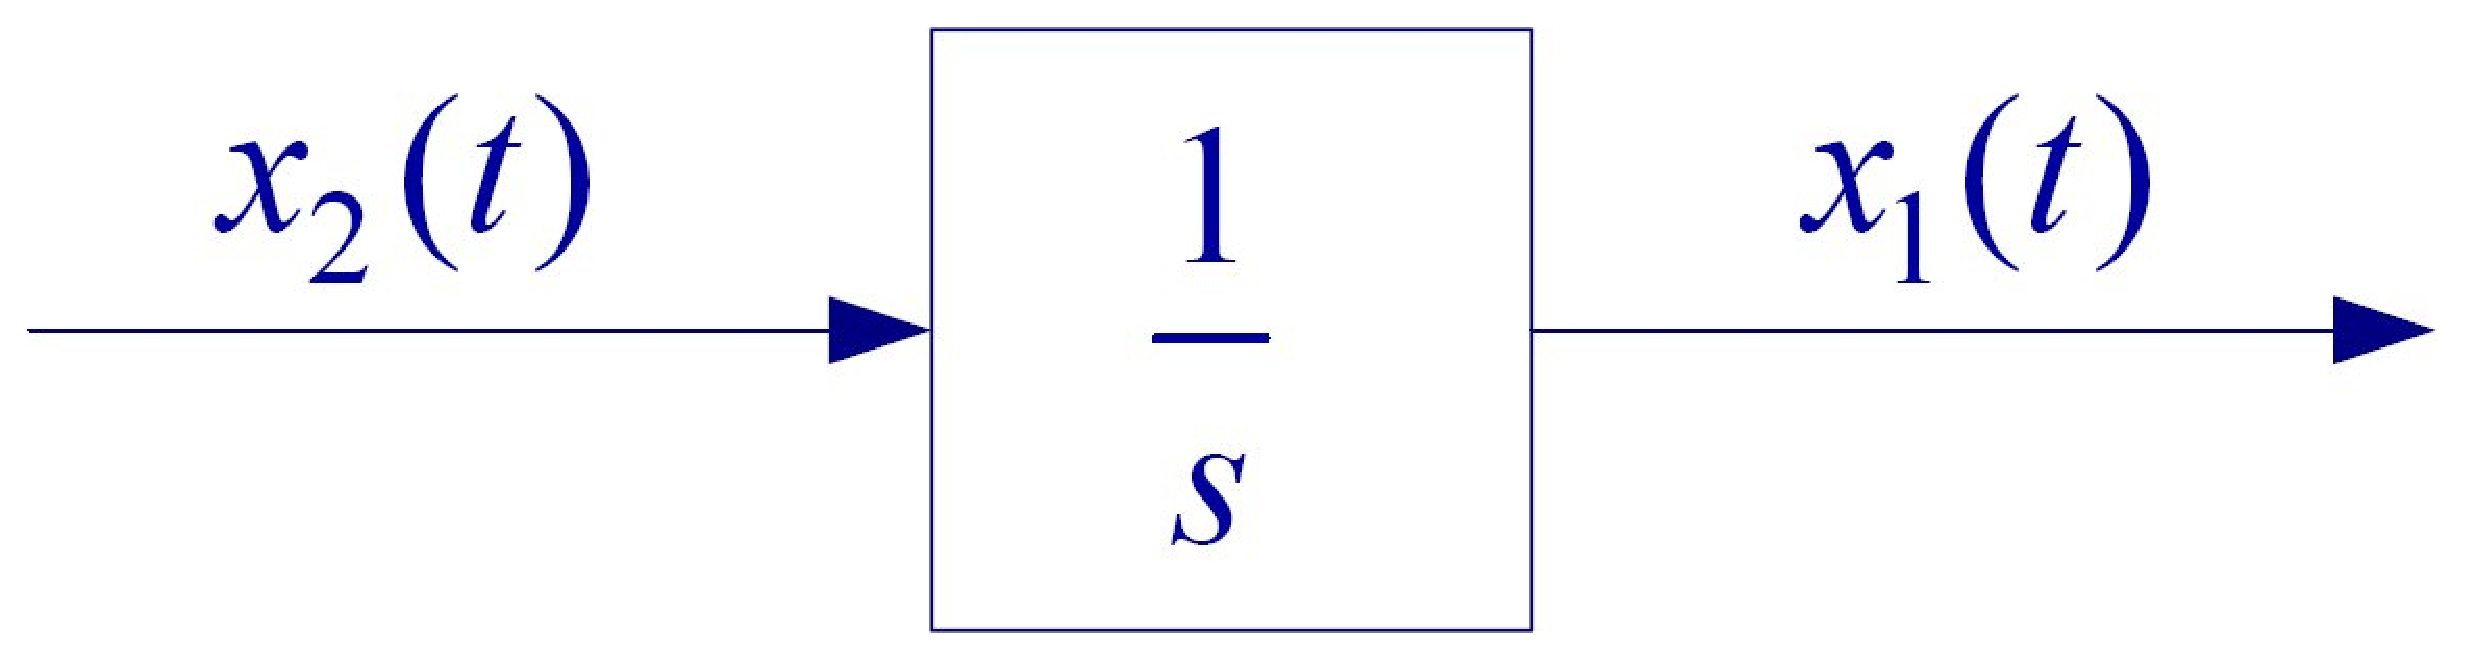
\includegraphics[width=.48\textwidth]{inttimedom}}
\sbox{\tempsmall}{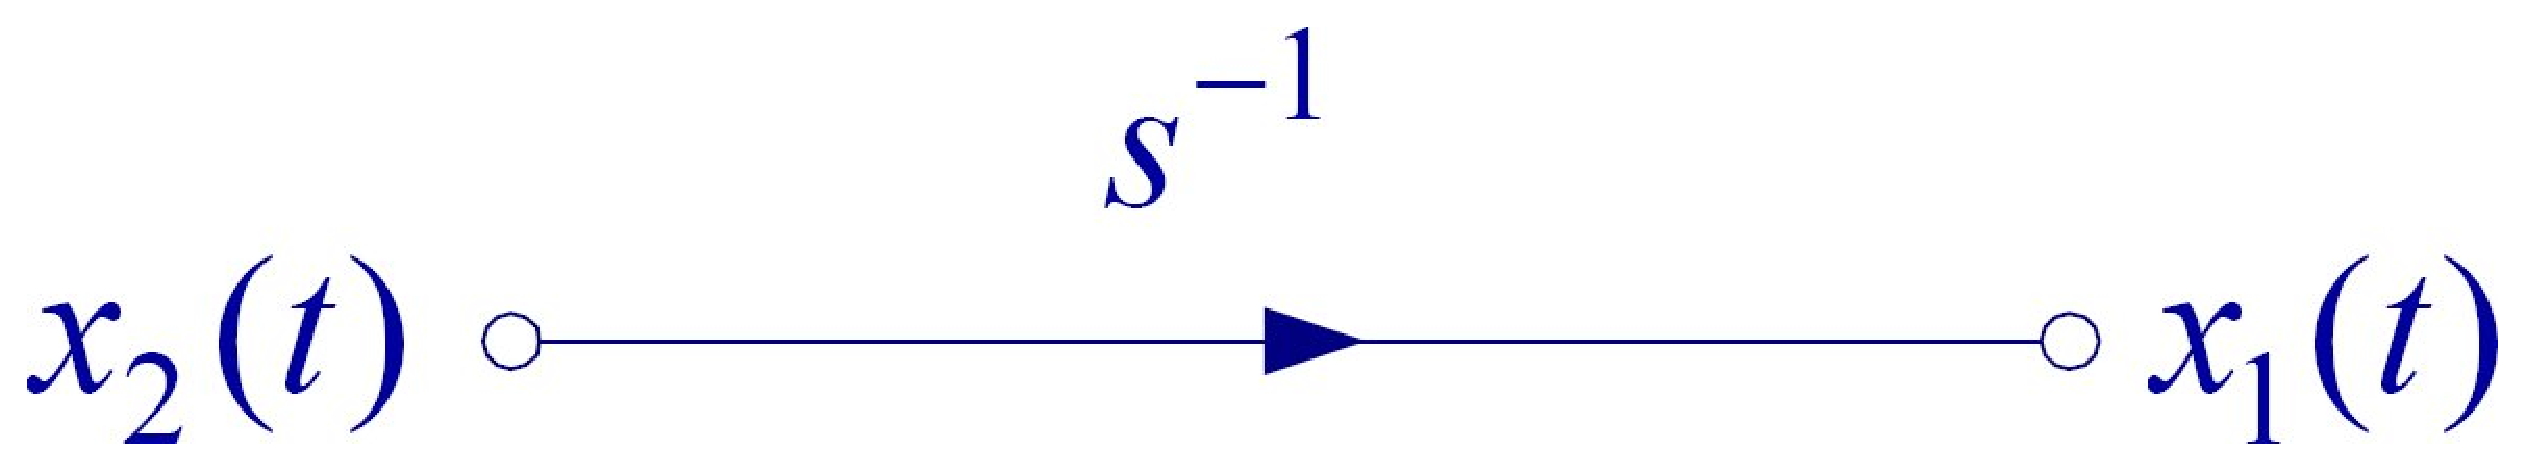
\includegraphics[width=.48\textwidth]{intsigflow}}
\newlength{\subfigoffset}
\setlength{\subfigoffset}{.5\ht\tempbig}
\addtolength{\subfigoffset}{-.5\ht\tempsmall}
\subfloat[Block diagram
            \label{fig.statespace.inttimedom}]{
            \usebox{\tempbig}
            }
\hfill
\subfloat[Signal flow graph
            \label{fig.statespace.intsigflow}]{
            \raisebox{\subfigoffset}{\usebox{\tempsmall}}
            }
\caption{\footnotesize
        Simulation diagrams: Graphical representations of state integrators in the time domain.
        \label{fig.statespace.integratorgraphs}
        }
\end{figure}
\par

It is important to know that that although the symbol $\frac{1}{s}$ is used for integration, the simulation diagram is still a time-domain representation.  The number of integrators is equal to the number of state variables.  For example, for the state equation in Example~\ref{ex.phasevarstatespace} we have three integrators in cascade, the three state variables are assigned to the output of each integrator as shown in Figure~\ref{fig.statespace.phasevardiagram}.  The final state equation---seen in (\ref{eq.dotstatesub})---is represented via a summing point and feedback paths.  Completing the output equation, we obtain the simulation diagram known as \uline{phase-variable control canonical form} (See Fig.\ \ref{fig.statespace.phasevardiagramsigflow}).

\begin{figure}[bht]
\centering
\sbox{\tempbig}{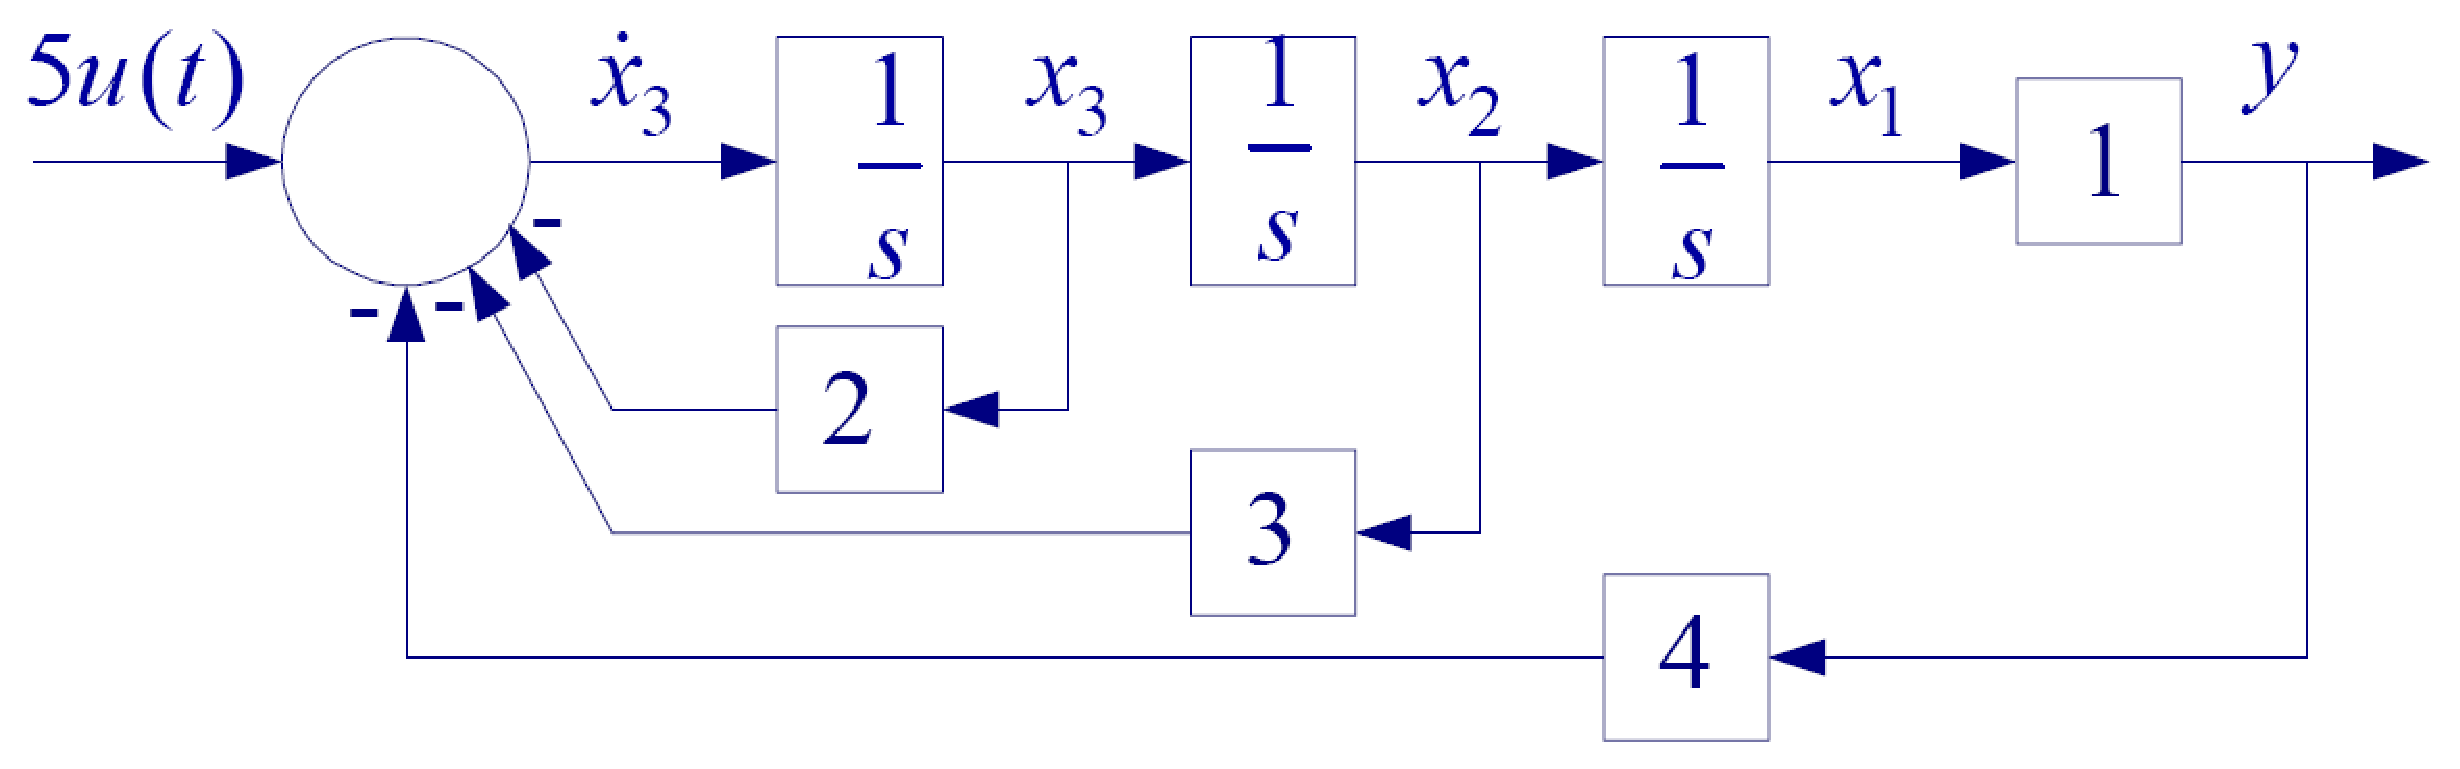
\includegraphics[width=.45\textwidth]{phasevarblock}}
\sbox{\tempsmall}{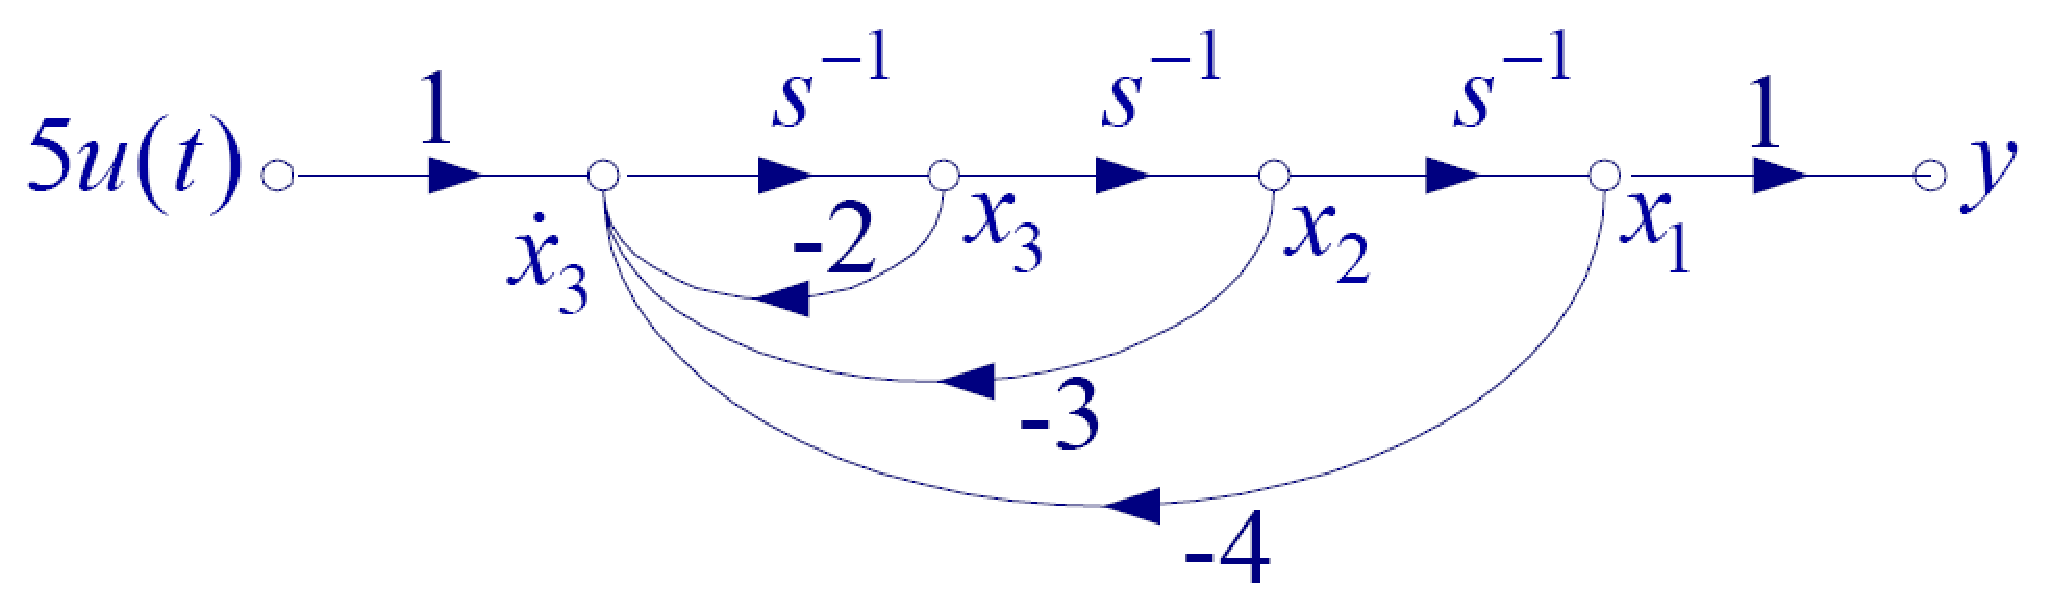
\includegraphics[width=.45\textwidth]{phasevarsigflow}}
\newlength{\subfigoffsetB}
\setlength{\subfigoffsetB}{.5\ht\tempbig}
\addtolength{\subfigoffsetB}{-.5\ht\tempsmall}
\subfloat[Block diagram]{
            \usebox{\tempbig}
            }
\hfill
\subfloat[Signal flow]{\label{fig.statespace.phasevardiagramsigflow}
            \raisebox{\subfigoffsetB}{\usebox{\tempsmall}}
            }
\caption{\footnotesize
        Simulation diagrams for Example~\ref{ex.phasevarstatespace} in phase-variable control canonical form.
        \label{fig.statespace.phasevardiagram}
        }
\end{figure}

\subsection{Transfer Function to State Space Conversion}

Consider the transfer function of a third-order system where the numerator degree is lower than that of the denominator.
\begin{equation}
    \frac{Y(s)}{U(s)} = \frac{b_2 s^2 + b_1 s + b_0}{
        s^3 + a_2 s^2 + a_1 s + a_0}
    \label{eq.thirdorderTF}
\end{equation}
The above transfer function is decomposed into two (frequency domain) blocks in Figure~\ref{fig.statespace.TFblockdecomp}.

\begin{figure}[bht]
\centering
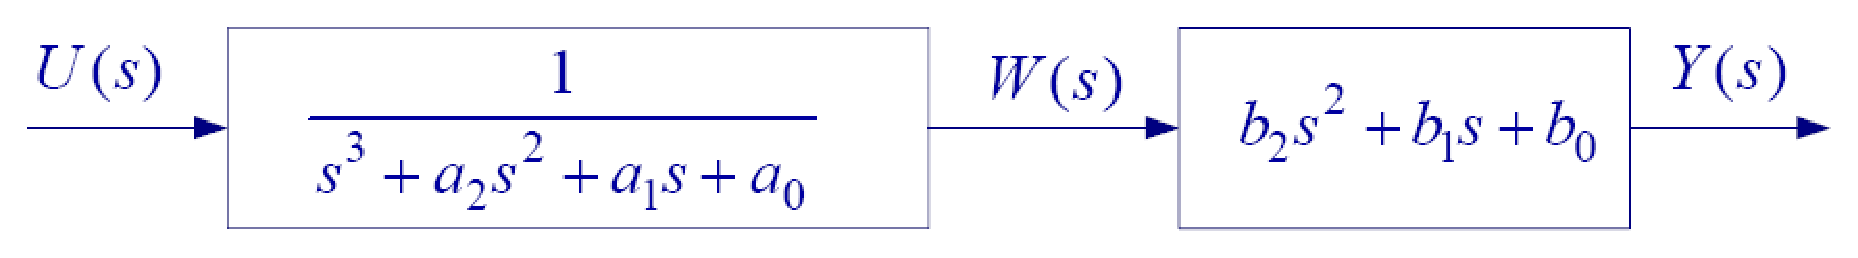
\includegraphics[width=0.8\textwidth]{TFblockdecomp}
\caption{\footnotesize
        The transfer function of Eq.\ (\ref{eq.thirdorderTF}) arranged in cascade form
        \label{fig.statespace.TFblockdecomp}
        }
\end{figure}

Denoting the output of the first block as $W(s)$, we have the following input/output relationships:
\begin{subequations}
\begin{gather}
    W(s) = \frac{U(s)}{s^3 + a_2 s^2 + a_1 s + a_0}
        \label{eq.inputstate} \\
    Y(s) = b_2 s^2 W(s) + b_1 s W(s) + b_0 W(s)
        \label{eq.outputstate}
\end{gather}
\end{subequations}
Rearranging Eq.\ (\ref{eq.inputstate}), we get
\begin{equation}
    s^3 W(s) = -a_2 s^2 W(s) - a_1 s W(s) - a_0 W(s) + U(s)
    \label{eq.inputstaterearrange}
\end{equation}
Using properties of frequency-domain tranforms, we see that Equations~(\ref{eq.inputstaterearrange}) and (\ref{eq.outputstate}) are the frequency-domain representations of the following time-domain differential equations:
\begin{subequations}
\begin{gather}
    \dddot{w} = -a_2 \ddot{w} - a_1 \dot{w} - a_0 w + u(t) \\
    y(t) = b_2 \ddot{w} + b_1 \dot{w} + b_0 w
\end{gather}
\end{subequations}

From the above expressions, we see that $\dddot{w}$ has to go through three integrators to get $w$ (as shown in Figure~\ref{fig.statespace.tripleintblock}).  Completing the above equations results in the phase-variable control canonical simulation diagram.

\begin{figure}[hbt]
\centering
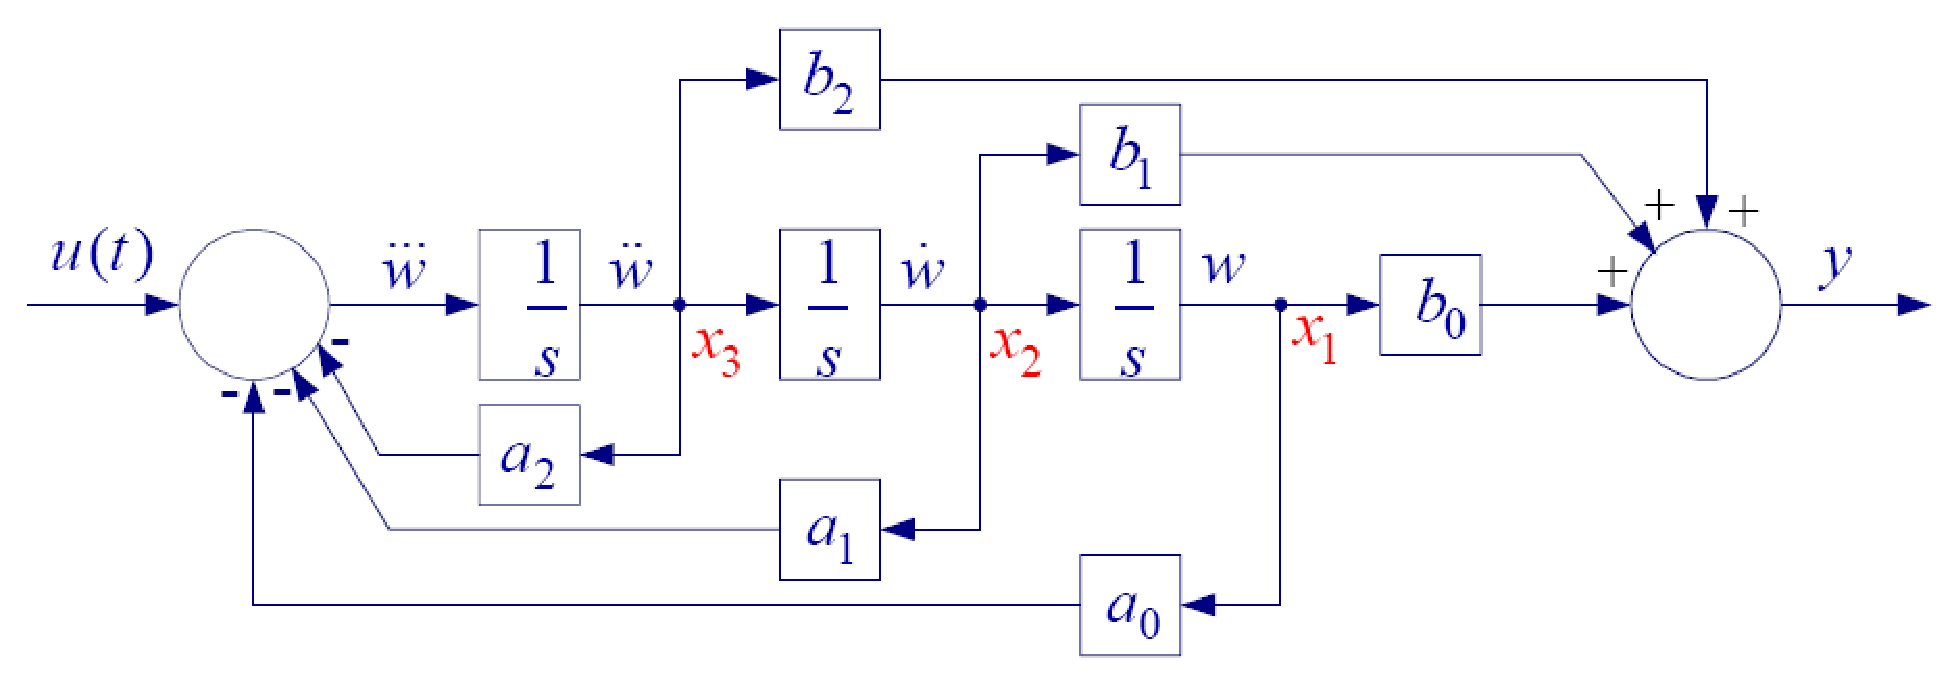
\includegraphics[width=.9\textwidth]{tripleintblock}
\caption{\footnotesize
        Phase variable control canonical simulation block diagram for the transfer function in Eq.~(\ref{eq.thirdorderTF})
        \label{fig.statespace.tripleintblock}
        }
\end{figure}

Figure~\ref{fig.statespace.tripleintblock} is a block diagram suitable for Simulink analysis.  You may find it easier to construct the simulation diagram similar to the signal flow graph as shown in Figure~\ref{fig.statespace.tripleintsigflow}.

\begin{figure}[thb]
\centering
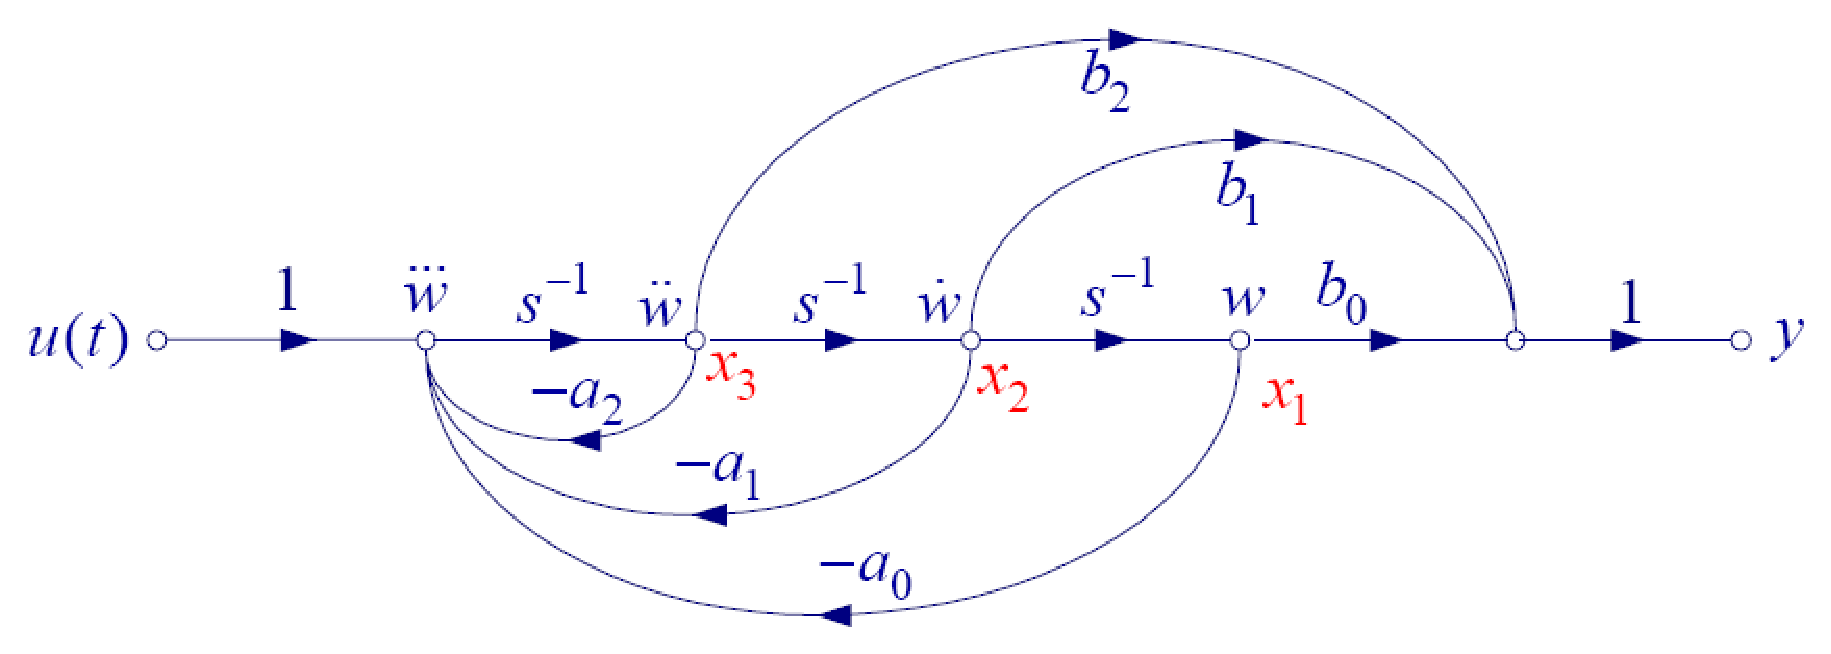
\includegraphics[width=0.9\textwidth]{tripleintsigflow}
\caption{\footnotesize
        Phase variable control canonical signal flow diagram for the transfer function in Eq.~(\ref{eq.thirdorderTF})
        \label{fig.statespace.tripleintsigflow}
        }
\end{figure}

In order to write the state equation, the state variables $x_1(t)$, $x_2(t)$, and $x_3(t)$ are assigned to the output of each integrator from right to left in Figs.\ \ref{fig.statespace.tripleintblock} and \ref{fig.statespace.tripleintsigflow}.  Next, an equation is written for the input of each integrator:
\begin{flalign*}
    \dot{x}_1 & = x_2 \\
    \dot{x}_2 & = x_3 \\
    \dot{x}_3 & = -a_0 x_1 -a_1 x_2 - a_2 x_3 + u(t)
\end{flalign*}
and the output equation is $y = b_0 x_1 + b_1 x_2 + b_2 x_3$.  Once again, lumping it into matrix form, we get
\begin{equation}
\begin{split}
    \left[ \begin{array}{c} \dot{x}_1 \\ \dot{x}_2 \\ \dot{x}_3
            \end{array} \right]
    & =
    \left[ \begin{array}{ccc} 0&1&0\\0&0&1\\-a_0&-a_1&-a_2
            \end{array} \right]
    \left[ \begin{array}{c} x_1 \\ x_2 \\ x_3
            \end{array} \right]
    +
    \left[ \begin{array}{c} 0 \\ 0 \\ 1
            \end{array} \right]
    u(t)
    \\
    y & =
    \left[ \begin{array}{ccc} b_0&b_1&b_2 \end{array} \right]
    \left[ \begin{array}{c} x_1 \\ x_2 \\ x_3
            \end{array} \right]
    \label{eq.tripleintstatespace}
\end{split}
\end{equation}

It is important to note that Mason's gain formula can be applied to the simulation diagram in Fig.\ \ref{fig.statespace.tripleintsigflow} to obtain the original transfer function.  Indeed, the determinant of the matrix $sI-A$ from Eq.~(\ref{eq.tripleintstatespace}) yields the characteristic equation (often denoted $\Delta$) for Mason's rule.  See Section 2.7 of \cite{dorf} for more on Mason's rule.
\par
In conclusion, it is important to remember that there is no unique state space representation for a given transfer function.  The state space often depends on the application involved, the complexity of the model, and the individual engineer!
\par
The Control System Toolbox in MATLAB contains a set of functions for model conversion.  Specifically, \verb#[A, B, C, D] = tf2ss(num,den)# converts the transfer function fraction to state space phase-variable control canonical form.

\pagebreak[4]
 %\setlength{\hsize}{.9\textwidth}
\begin{workex} \label{ex.TFtoSS}
\begin{equation*}
    G(s) = \frac{Y(s)}{U(s)} =
        \frac{s^2 + 7s + 2}{s^3 + 9s^2 + 26s + 24}
\end{equation*}

For the above transfer function, do the following:
\begin{enumerate}
    \item Draw the simulation diagram and find a state space representation.
    \item Use the MATLAB Control System Toolbox function \texttt{tf2ss} to find a state model.
\end{enumerate}
\textit{Solution}:
\par
1. The transfer function in block diagram cascade form looks like Figure~\ref{fig.ex.statespace.TFblock}.
\par
From this we have
\begin{flalign*}
    s^3W(s) &= -9Ws^2W(s) - 26sW(s) - 24W(s) + U(s) \\
    Y(s)    &= s^2W(s) + 7sW(s) +2W(s)
\end{flalign*}
Converting these to the time domain:
\begin{flalign*}
    \dddot{w}   &= -9\ddot{w} - 26\dot{w} - 24w + u \\
    y(t)        &= \ddot{w} + 7\dot{w} + 2w
\end{flalign*}
The time-domain equations above yield the simulation diagram in Figure~\ref{fig.ex.statespace.TFsigflow}.
\par
To obtain the state equation, the state variables $x_1(t)$, $x_2(t)$, and $x_3(t)$ are assigned to the output of each integrator from right to left.  The equations corresponding to the input of each integrator are:
\begin{flalign*}
    \dot{x}_1 & = x_2 \\
    \dot{x}_2 & = x_3 \\
    \dot{x}_3 & = -24x_1 - 26x_2 - 9x_3 + u(t)
\end{flalign*}
The output equation is the summation of the feedforward links: $y = 2x_1 + 7x_2 +x_3$.
\par
Finally, in matrix form we have
\begin{flalign*}
    \left[ \begin{array}{c} \dot{x}_1 \\ \dot{x}_2 \\ \dot{x}_3
            \end{array} \right]
    & =
    \left[ \begin{array}{ccc} 0&1&0\\0&0&1\\-24&-26&-9
            \end{array} \right]
    \left[ \begin{array}{c} x_1 \\ x_2 \\ x_3
            \end{array} \right]
    +
    \left[ \begin{array}{c} 0 \\ 0 \\ 1
            \end{array} \right]
    u(t)
    \\
    y & =
    \left[ \begin{array}{ccc} 2&7&1 \end{array} \right]
    \left[ \begin{array}{c} x_1 \\ x_2 \\ x_3
            \end{array} \right]
\end{flalign*}
2. We write the following statements to check our results in MATLAB:
\begin{verbatim}
>> num = [1 7 2]; den = [1 9 26 24];
>> [A, B, C, D] = tf2ss(num,den)
A =                 B =         C =             D =
    -9  -26 -24         1           1   7   2       0
    1   0   0           0
    0   1   0           0
>>
\end{verbatim}
\end{workex}
\par
It is important to realize that parts 1 and 2 of Example~\ref{ex.TFtoSS} are equivalent.  MATLAB simply numbers the state variables in a different order.  To confirm this, we need only perform a simple substitution for one set of state variables.

\begin{figure}[bht]
\centering
\subfloat[Block diagram of the transfer function in cascade
        \label{fig.ex.statespace.TFblock}]{
        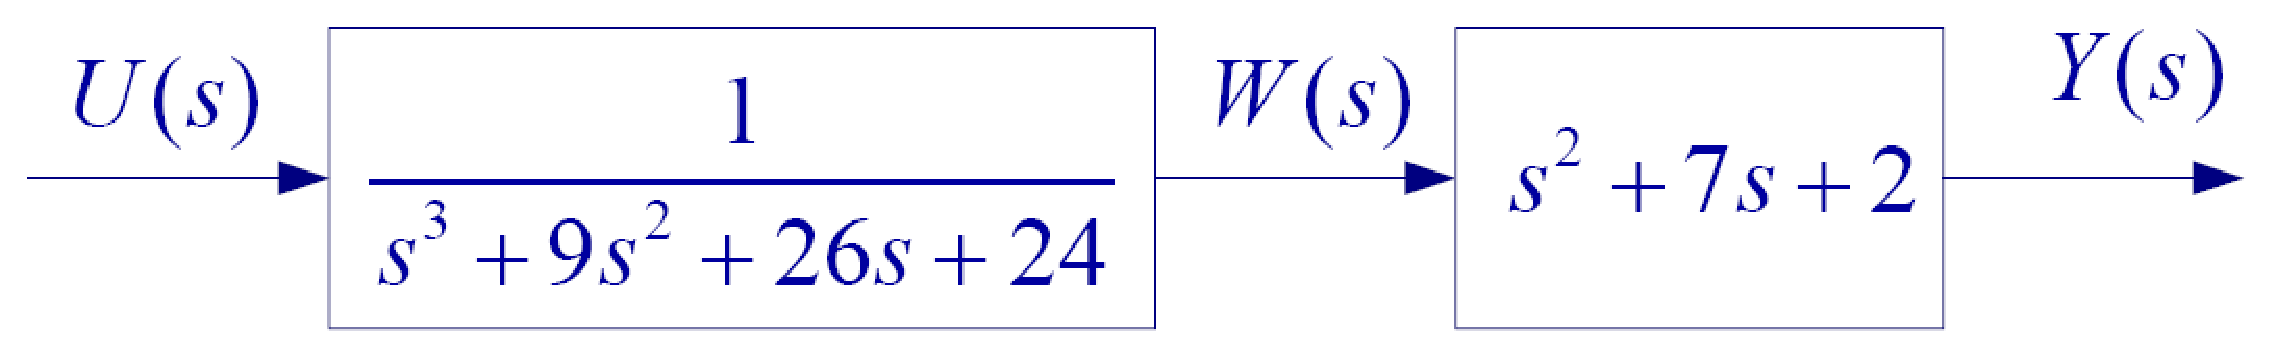
\includegraphics[width=0.7\textwidth]{TFtoSSblock}
        }
\newline
\subfloat[Signal flow simulation digram
        \label{fig.ex.statespace.TFsigflow}]{
        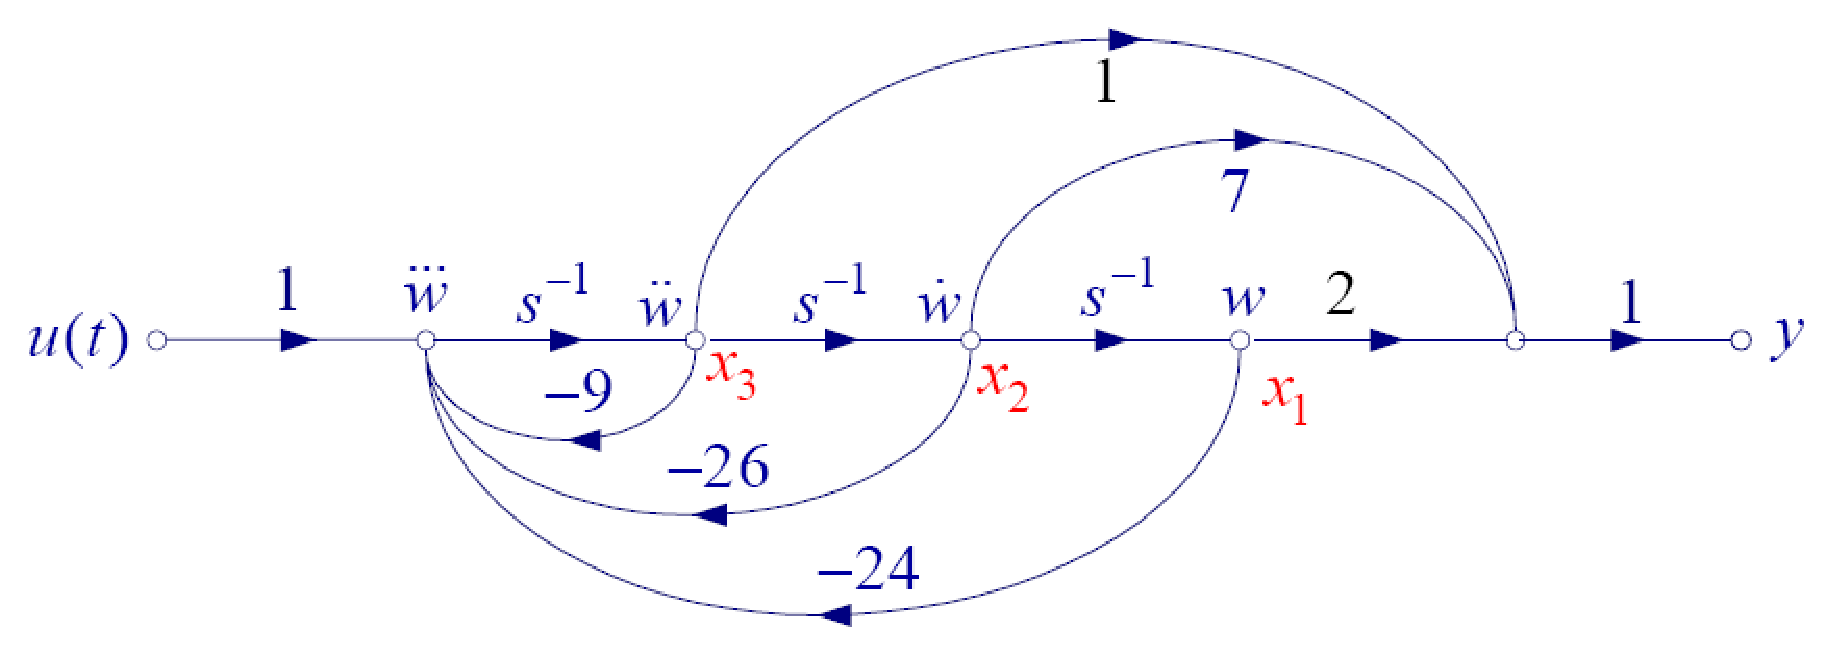
\includegraphics[width=0.8\textwidth]{TFtoSSsigflow}
        }
\caption{\footnotesize
        Diagrams for Example~\ref{ex.TFtoSS}
        }
\end{figure}

\subsection{State Space to Transfer Function Conversion}
Consider the state equation (\ref{eq.stateeq}).  We may take its Laplace transform and rearrange it as follows:
\begin{equation*}
    sX(s) = AX(s) + BU(s) \Rightarrow (sI - A)X(s) = BU(s)
\end{equation*}
If we combine this with the transform of the output equation: $Y(s) = CX(s) + DU(s)$, we get
\begin{equation*}
    Y(s) = C(sI - A)^{-1} BU(s) + DU(s)
\end{equation*}
or, equivalently
\begin{equation}
    \frac{Y(s)}{U(s)} = C(sI-A)^{-1} B+D
    \label{eq.TFfromSS}
\end{equation}
\par
In the Control Systems Toolbox, the command \verb#[num, den] = ss2tf(A,B,C,D,i)# converts the state equation to a transfer function for the $i^{th}$ input.

\begin{workex} \label{ex.SStoTF}
\begin{flalign*}
    \left[ \begin{array}{c} \dot{x}_1 \\ \dot{x}_2
            \end{array} \right]
    & =
    \left[ \begin{array}{cc} 0&1\\-6&-5
            \end{array} \right]
    \left[ \begin{array}{c} x_1 \\ x_2
            \end{array} \right]
    +
    \left[ \begin{array}{c} 0  \\ 1
            \end{array} \right]
    u(t)
    \\
    y & =
    \left[ \begin{array}{cc} 8&1 \end{array} \right]
    \left[ \begin{array}{c} x_1 \\ x_2
            \end{array} \right]
\end{flalign*}
Obtain the transfer function for the system described in the above state space model.\\
\textit{Solution}:
\par
Use the formula in Eq.\ (\ref{eq.TFfromSS}).
\begin{flalign*}
    sI - A &= \left[ \begin{array}{cc} s & -1 \\ 6 & s+5
                        \end{array} \right] \\
    \Rightarrow \Phi(s) := (sI - A)^{-1} &=
        \frac{\left[ \begin{array}{cc} s+5 & 1 \\ -6 & s
                        \end{array} \right]}{s^2+5s+6} \\
    \Rightarrow G(s) := C(sI-A)^{-1}B &=
        \left[ \begin{array}{cc} 8&1 \end{array} \right]
        \frac{\left[ \begin{array}{cc} s+5 & 1 \\ -6 & s
                        \end{array} \right]
                        \left[ \begin{array}{c}0\\1\end{array}\right]}
                        {s^2+5s+6} \\
    &= \frac{\left[ \begin{array}{cc} 8&1 \end{array} \right]
                \left[ \begin{array}{c}1\\s\end{array}\right]}
            {s^2+5s+6}
\end{flalign*}
Therefore the transfer function is
\begin{equation*}
    G(s) = \frac{s+8}{s^2+5s+6}
\end{equation*}
\end{workex}

\begin{workex} \label{ex.SStoTFmatlab}
\begin{flalign*}
    \left[ \begin{array}{c} \dot{x}_1 \\ \dot{x}_2 \\ \dot{x}_3
            \end{array} \right]
    & =
    \left[ \begin{array}{ccc} 0&1&0\\0&0&1\\-1&-2&-3
            \end{array} \right]
    \left[ \begin{array}{c} x_1 \\ x_2 \\ x_3
            \end{array} \right]
    +
    \left[ \begin{array}{c} 10 \\ 0 \\ 0
            \end{array} \right]
    u(t)
    \\
    y & =
    \left[ \begin{array}{ccc} 1&0&0 \end{array} \right]
    \left[ \begin{array}{c} x_1 \\ x_2 \\ x_3
            \end{array} \right]
\end{flalign*}
Use MATLAB to find the transfer function corresponding to the above state space model.\\
\textit{Solution}:
\begin{verbatim}
>> A = [0 1 0; 0 0 1; -1 -2 -3]; B = [10; 0; 0];
>> C = [1 0 0]; D = [0];
>> [num, den] = ss2tf(A,B,C,D,1);
>> G = tf(num,den)
G =
    10 s^2 + 30 s + 20
   ---------------------
   s^3 + 3 s^2 + 2 s + 1
>>
\end{verbatim}
\end{workex}

Also, \verb#[z, p, k] = ss2zp(A,B,C,D,i)# converts the state equations to the transfer function in factored form.
\par
MATLAB's Control System Toolbox contains many functions for model creation and inversion, data extraction, and system interconnections.  A few of these functions for continuous-time control systems are listed in Table~\ref{tab.statespace.ConSysTool}.  For a complete list of the toolbox's functions, type \verb=help/control/control= at the command prompt.

\begin{table}[bht]
\centering
\begin{tabular}{c|p{0.6\textwidth}}
    \textit{Command}& \multicolumn{1}{c}{\textit{Description}}\\ \hline \hline
    \verb=tf=       &   Create transfer function models \\
    \verb=zpk=      &   Create zero/pole/gain models \\
    \verb=ss=       &   Create state space models \\
    \verb=tfdata=   &   Extract numerators and denominators \\
    \verb=zpkdata=  &   Extract zero/pole/gain data \\
    \verb=ssdata=   &   Extract state space matrices \\
    \verb=append=   &   Group LTI systems by appending inputs and outputs \\
    \verb=parallel= &   Generalized parallel connection \\
    \verb=series=   &   Generalized series connection \\
    \verb=feedback= &   Feedback connection of two systems \\
    \verb=connect=  &   Derive state space model from block diagram description \\
    \verb=blkbuild= &   Builds a model from a block diagram
\end{tabular}
\caption{\footnotesize
        Important continuous-time control system commands
        \label{tab.statespace.ConSysTool}
        }
\end{table}

The Control System Toolbox supports three commonly used representations of linear time-invariant (LTI) systems: \verb=tf=, \verb=zpk=, and \verb=ss= objects.  To create an LTI model or object, use the corresponding constructor. For example, \verb#sys = tf(1,[1 0])# creates the transfer function $H(s) = 1/s$.  The resulting variable \verb=sys= is a \verb=tf= object containing the numerator and denominator data.  You can now treat the entire model as a single MATLAB variable.  For more details and examples on how to specify the various types of LTI models, type \verb=ltimodels= followed by the construct type at the MATLAB command prompt.
\par
The functions \verb=tfdata=, \verb=zpkdate=, and \verb=ssdata= are provided for extracting the parameters of their corresponding objects.  For example, the command \verb#[num, den] = tfdata(T,'v')# returns the numerator and denominator of the \verb=tf= object \verb=T=.  The argument \verb='v'= formats the outputs as row vectors rather than cell arrays.
\par
The Control System Toolbox contains many more commands that allow the construction of a system out of its components.  The lower entries in Table~\ref{tab.statespace.ConSysTool} are useful for this purpose.

\begin{figure}[thb]
\centering
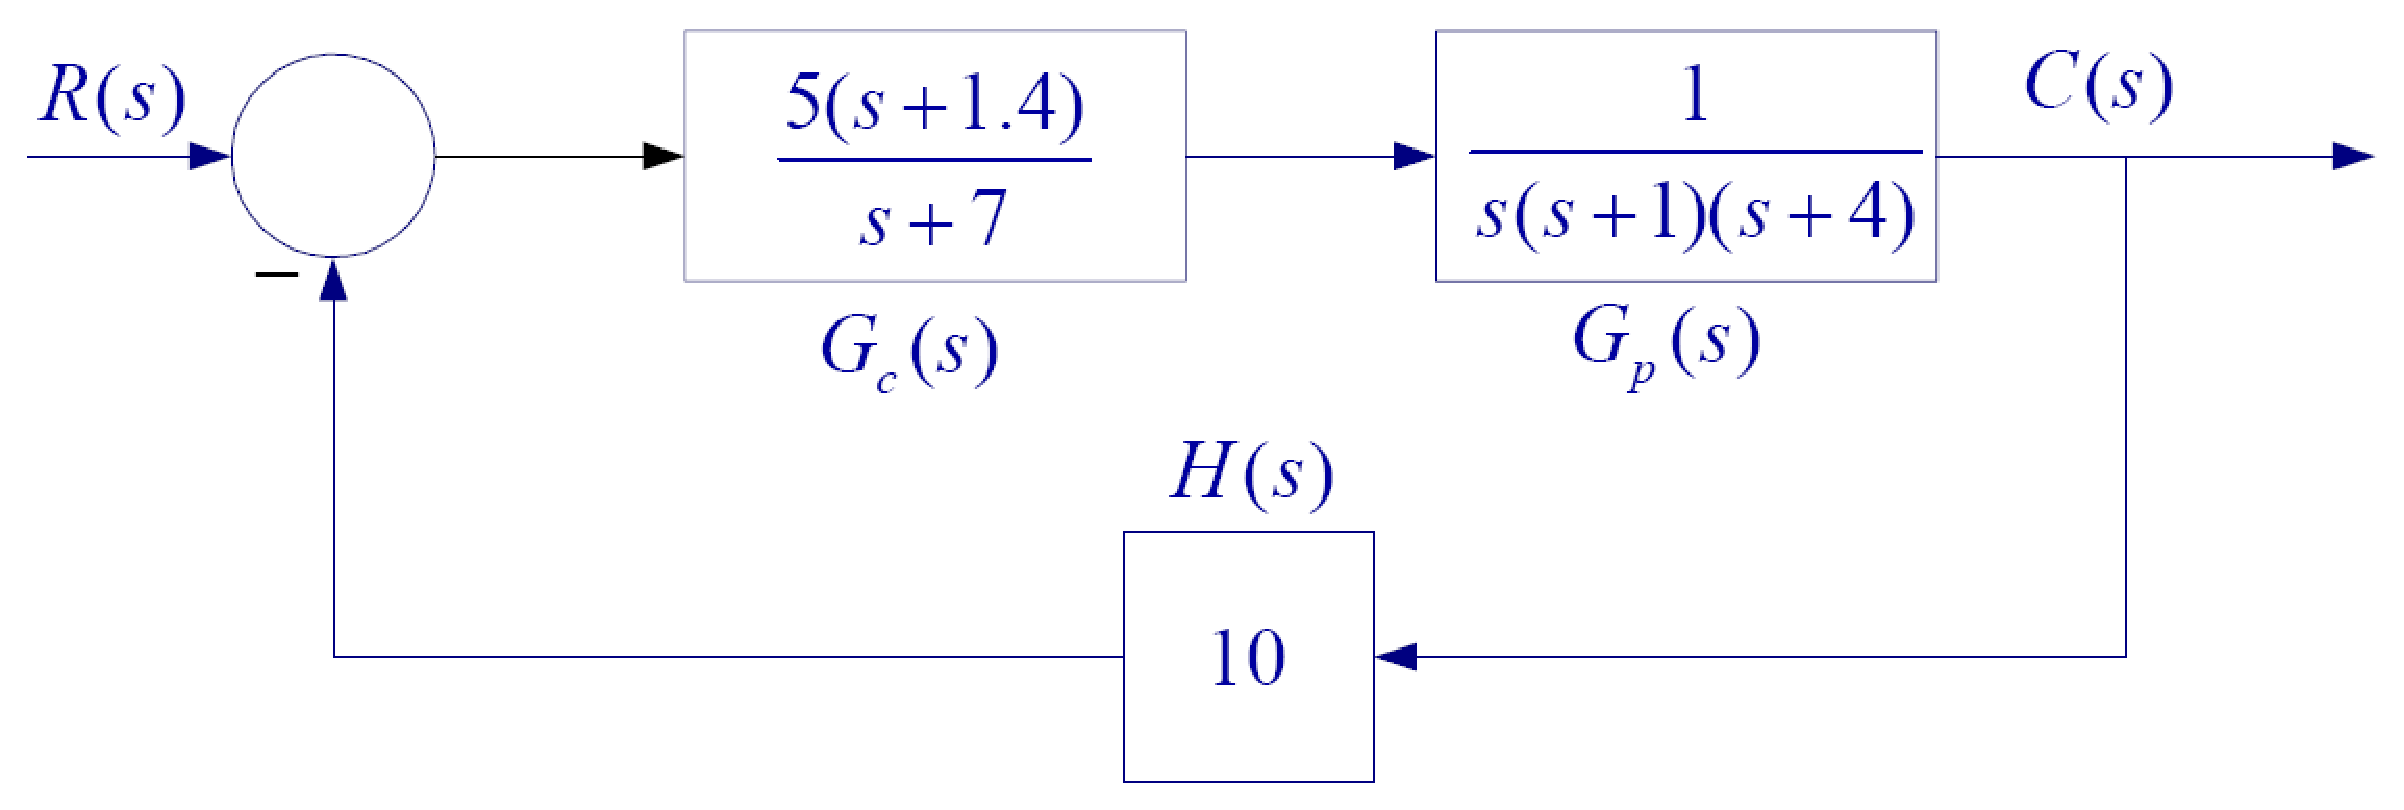
\includegraphics[width=.8\textwidth]{buildfeedback}
\caption{\footnotesize
        Block diagram in the frequency domain for the system in Example~\ref{ex.buildfeedback}.
        \label{fig.statespace.buildfeedback}
        }
\end{figure}

\begin{workex} \label{ex.buildfeedback}
Use the \verb=feedback= function to obtain the closed-loop transfer function and the \verb=tf2ss= function to obtain the closed-loop state space model of the system in Figure~\ref{fig.statespace.buildfeedback}.\\
\textit{Solution}:\\
The following commands should produce the desired result:
\begin{verbatim}
Gc = tf(5*[1 1.4],[1 7]);       % transfer function Gc
Gp = tf([1],[1 5 4 0]);         % transfer function Gp
H = 10;
G = series(Gc,Gp)               % connect Gc and Gp in cascade
T = feedback(G,H)               % close feedback loop
[num, den] = tfdata(T,'v')      % return num and den as row vectors
[A, B, C, D] = tf2ss(num,den)   % converts to state space model
\end{verbatim}

The transfer function should look like
\begin{verbatim}
                5 s + 7
     ---------------------------------
      s^4 12 s^3 + 39 s^2 + 78 s + 70
\end{verbatim}

And the matrices are
\begin{verbatim}
A =                     B =     C =                 D =
    -12 -39 -78 -70         1       0   0   5   7       0
    1   0   0   0           0
    0   1   0   0           0
    0   0   1   0           0
\end{verbatim}
\end{workex}

\section{MATLAB Functions for Modeling and Analysis}
Once a system is described by a certain model---be it in state space, by a transfer function, or otherwise---it is often important to perform some form of analysis on it.  How does it respond to different initial conditions?  Which inputs correspond to which outputs?  Is this thing stable or can we make it stable?  These are all questions we may ask of a system that comes presented to us as a ``black box.''
\par
The MATLAB Control System Toolbox contains the functions in Table~\ref{tab.statespace.ConSysToolTime} for analysis of time-domain response.

\begin{table}[bht]
\centering
\renewcommand{\arraystretch}{1.2}
\begin{tabular}{c|p{0.55\textwidth}}
    \textit{Command}& \multicolumn{1}{c}{\textit{Description}}\\ \hline \hline
    \verb=step=         &   Step response \\
    \verb=impulse=      &   Impulse response \\
    \verb=initial=      &   Response of a state space system to the given
                                initial state \\
    \verb=lsim=         &   Response to arbitrary inputs \\
    \verb=gensig=       &   Generates input signal for \verb=lsim= \\
    \verb=damp=         &   Natural frequency and damping of system poles \\
    \verb=ltiview=      &   Response analysis GUI (LTI System Viewer)
\end{tabular}
\caption{\footnotesize
        Time-domain system analysis functions
        \label{tab.statespace.ConSysToolTime}
        }
\end{table}
\par
Given a transfer function of a closed-loop control system, the function \verb=step(num,den)= produces the step response plot with the time vector automatically determined.  If the closed-loop system is defined in state space instead, we use \verb=step(A,B,C,D)= with or without subsequent optional arguments.  If output variables are specified for the \verb=step= function, say \verb=[y, t, x]=, then the output will be saved to \verb=y= for the time vector \verb=t=.  The array \verb=x= contains the trajectories of all of the state variables along the same time vector.  This syntax also applies to \verb=impulse=, \verb=initial=, and \verb=lsim=.

\vspace{6pt}
\begin{workex}  \label{ex.unitstep}
\begin{equation*}
    \frac{C(s)}{R(s)} =
        \frac{25(1+0.4s)}{ (1+0.16x)(x^2+6s+25)}
\end{equation*}
Obtain the unit step response of the system with the closed-loop transfer function above.  Also, use the \verb=damp= function to obtain the roots of the characteristic equation, the corresponding damping factors, and the natural frequencies.\\
\textit{Solution}:\\
The following code produces the response seen in Figure~\ref{fig.ex.unitstep}.
\begin{verbatim}
>> num = 25*[0.4 1];
>> den = conv([0.16 1], [1 6 25])   % Multiplies two polynomials.
>> T = tf(num,den)                  % Create TF object.
>> step(T), grid                    % Produces step response plot.
>> damp(T)                          % Produces data below:
        Eigenvalue              Damping         Freq. (rad/s)
        -3 + 4i                 6.00e-001           5.00
        -3 - 4i                 6.00e-001           5.00
        -6.25                   1.00e+000           6.25
>>
\end{verbatim}
The damping factors and natural frequencies are displayed in the right two columns.  The eigenvalues are the roots of the characteristic equation.
\end{workex}

\begin{figure}[thb]
\centering
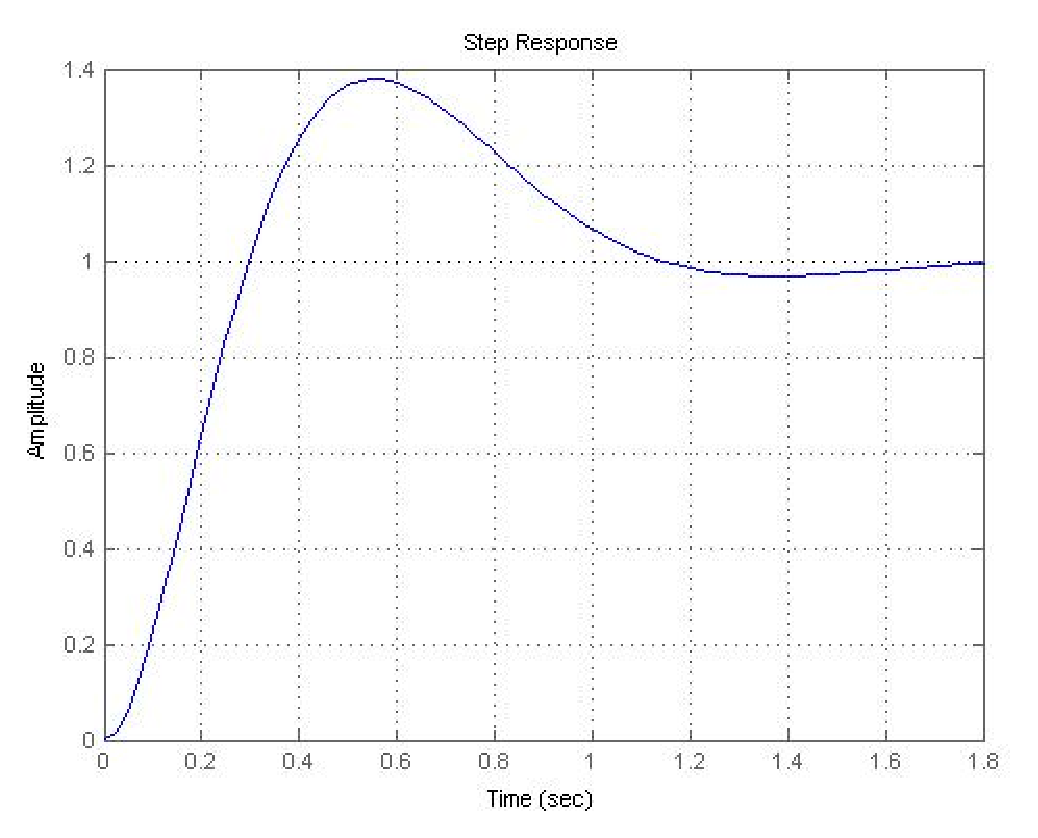
\includegraphics[width=.75\textwidth]{unitstep}
\caption{ \footnotesize
        Unit step response for system in Example \ref{ex.unitstep}
        \label{fig.ex.unitstep}
        }
\end{figure}

\begin{workex}  \label{ex.dompoles}
\begin{equation*}
    \frac{C(s)}{R(s)} = T(s) =
        \frac{750}{s^3 + 36s^2 + 205s + 750}
\end{equation*}
The closed-loop transfer function of a control system is described by the third-order transfer function $T(s)$.  Do the following:
\begin{enumerate}
\item
    Find the dominant poles of the system.
\item
    Find a reduced-order model.
\item
    Obtain the step response of the third-order system and the reduced-order system on the same figure plot.
\end{enumerate}
\textit{Solution}:\\
1. The poles are the roots of the denominator polynomial.  To find this, we use \verb=roots([1 36 205 750])=.  This gives us roots at $-30$ and $-3\pm4i$.  To determine dominance, we look at the time constants (negative inverse of real part) associated with these poles.  We see the pole at $-30$ has time constant $\tau_1 = 1/30$ where as the other two have time constant $\tau_2 = 1/3$.  The order of magnitude difference tells us that the poles at $3\pm4i$ are dominant. For more on time constants, see~\cite{dorf}, Section~2.5.\\
2. To reduce the model, we factor out the negligible pole and divide the numerator by its magnitude:
\begin{equation*}
    T(s) = \frac{750}{(s+30)(s^2 + 6s + 25)}
        \Rightarrow \tilde{T}(s) = \frac{25}{s^2 + 6s + 25}
\end{equation*}
\end{workex}\\
\begin{codex}
3. The following script produces the desired plot (Fig.\ \ref{fig.ex.dompoles}).
\begin{verbatim}
num1 = 750;
den1 = [1 36 205 750];
T = tf(num1,den1);              % Third-order system tf object.
num2 = 25;
den2 = [1 6 25];
Ttilde = tf(num2,den2);         % Reduced system tf object.
[y1 t] = step(T);               % Response and time vectors of T.
y2 = step(Ttilde,t);            % Response using the same time
                                    % vector of the reduced system.
plot(t,y1,'r-',t,y2,'b:')       % Put responses on the same plot.
grid;
xlabel('Time (s)');
ylabel('Displacement');
legend('Third-order','Reduced-order');
\end{verbatim}
\end{codex}

\begin{figure}[bht]
\centering
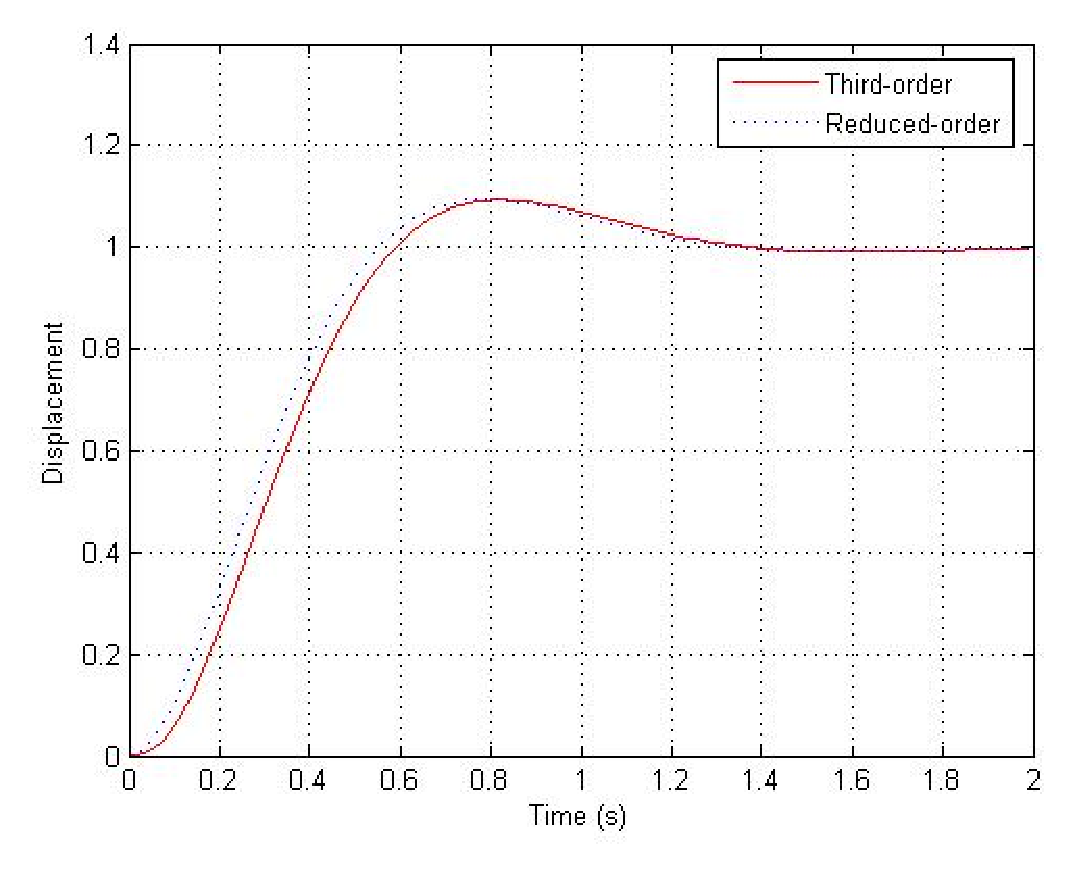
\includegraphics[width=.9\textwidth]{dompoles}
\caption{ \footnotesize
        Step responses of the original and reduced systems in Example~\ref{ex.dompoles}
        \label{fig.ex.dompoles}
        }
\end{figure}

\subsection{The LTI Viewer}
The Control System Toolbox LTI Viewer is a GUI (graphical user interface) that visually demonstrates the analysis of linear time-invariant systems.  We use the LTI Viewer to view and compare the response plots of several linear models at the same time.  We can also generate time- and frequency-domain response plots to inspect key response parameters such as rise time, maximum overshoot, and stability margins.  Using mouse-driven interactions, we can select input and output channels for multi-input, multi-output (MIMO) systems.  The LTI Viewer can display up to six different plot types simultaneously, including step and impulse responses, Bode, Nyquist, Nichols, sigma, and pole/zero diagrams.
\par
The command syntax is
\begin{verbatim}
ltiview('plot type',sys,extra)
\end{verbatim}
where \verb=sys= is the system object in question, and \verb='plot type'= is one of the following strings: \verb=step=, \verb=impulse=, \verb=initial=, \verb=lsim=, \verb=bode=, \verb=nyquist=, \verb=nichols=, or \verb=sigma=.  The optional argument \verb=extra= specifies the final time of the simulation.
\par
Once an LTI Viewer is open, a right-click of the mouse allows us to change the response type and obtain the system time-domain and frequency-domain specifications, such as those in Table~\ref{tab.ltiview}.

\begin{table}[bht]
\centering
\renewcommand{\arraystretch}{1.2}
\begin{tabular}{c|p{0.55\textwidth}}
    \textit{Menu Title}& \multicolumn{1}{c}{\textit{Description}}\\ \hline \hline
    Plot Type       &   Changes the plot type \\
    Systems         &   Selects any of the models loaded in the LTI Viewer \\
    Characteristics &   Displays key response characteristics and parameters\\
    Zoom            &   Zooms in and out of plot regions \\
    Grid            &   Adds grids to the plots \\
    Properties      &   Opens the Property Editor to customize plot attributes
\end{tabular}
\caption{\footnotesize
        LTI Viewer context-click menus
        \label{tab.ltiview}
        }
\end{table}

\begin{figure}[thb]
\centering
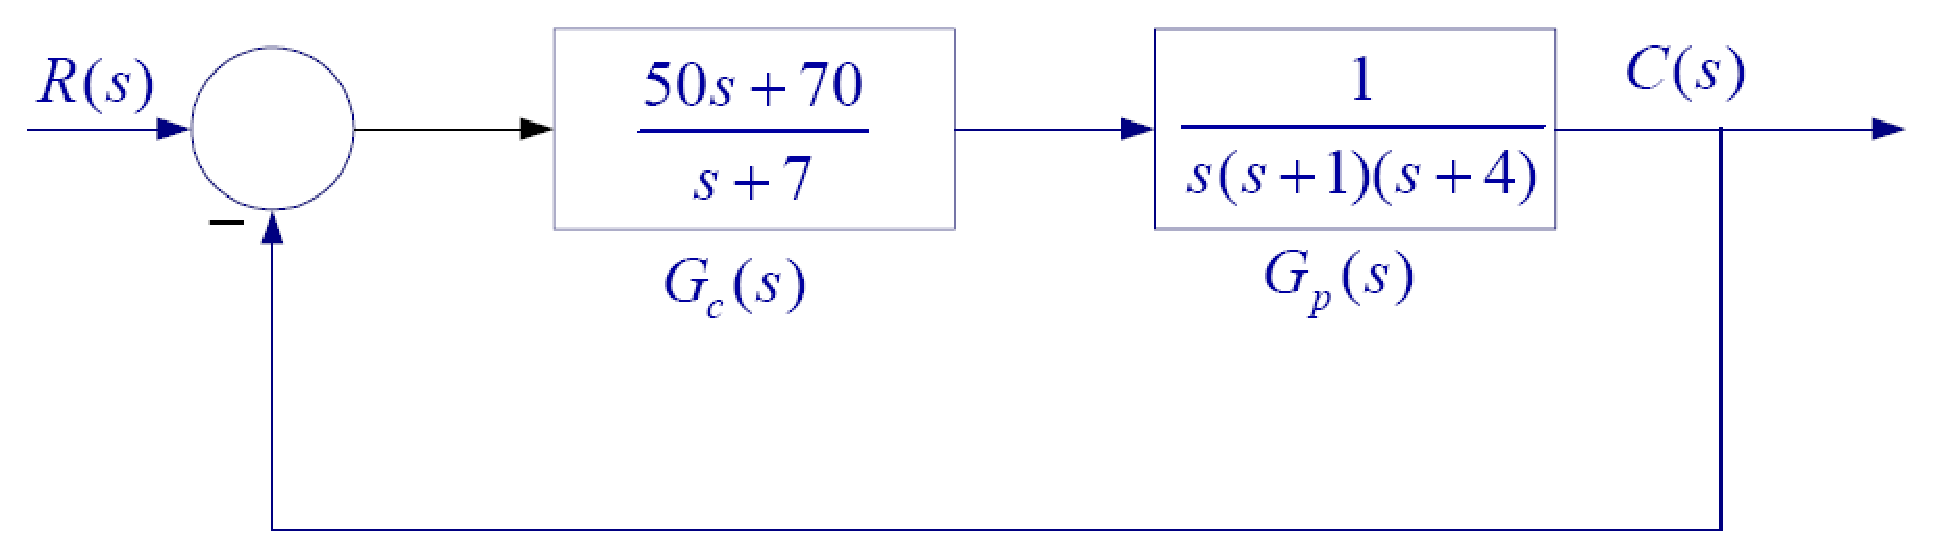
\includegraphics[width=.7\textwidth]{ltiviewexample}
\caption{ \footnotesize
        Block diagram for Example~\ref{ex.ltiview}
        \label{fig.ex.ltiview}
        }
\end{figure}

\begin{workex}  \label{ex.ltiview}
Use the LTI Viewer to obtain the step response and the time-domain specifications for the control system shown in Fig.\ \ref{fig.ex.ltiview}.\\
\textit{Solution}:\\
We use the following commands to generate the response plot in Figure~\ref{fig.ex.ltiviewstep}.
\begin{verbatim}
>> Gc = tf([50 70],[1 7]);      % Transfer function Gc.
>> Gp = tf([1],conv([1 1 0],[1 4]));    % Transfer function Gp,
                                % with expanded denominator.
>> H = 1;                       % Unity feedback.
>> G = series(Gc,Gp);           % Connect Gc and Gp in cascade.
>> T = feedback(G,H)            % Close unity feedback loop.

Transfer function:
            50 s + 70
---------------------------------
s^4 + 12 s^3 + 39 s^2 + 78 s + 70

>> ltiview('step',T)
>>
\end{verbatim}
\end{workex}

\begin{figure}[bht]
\centering
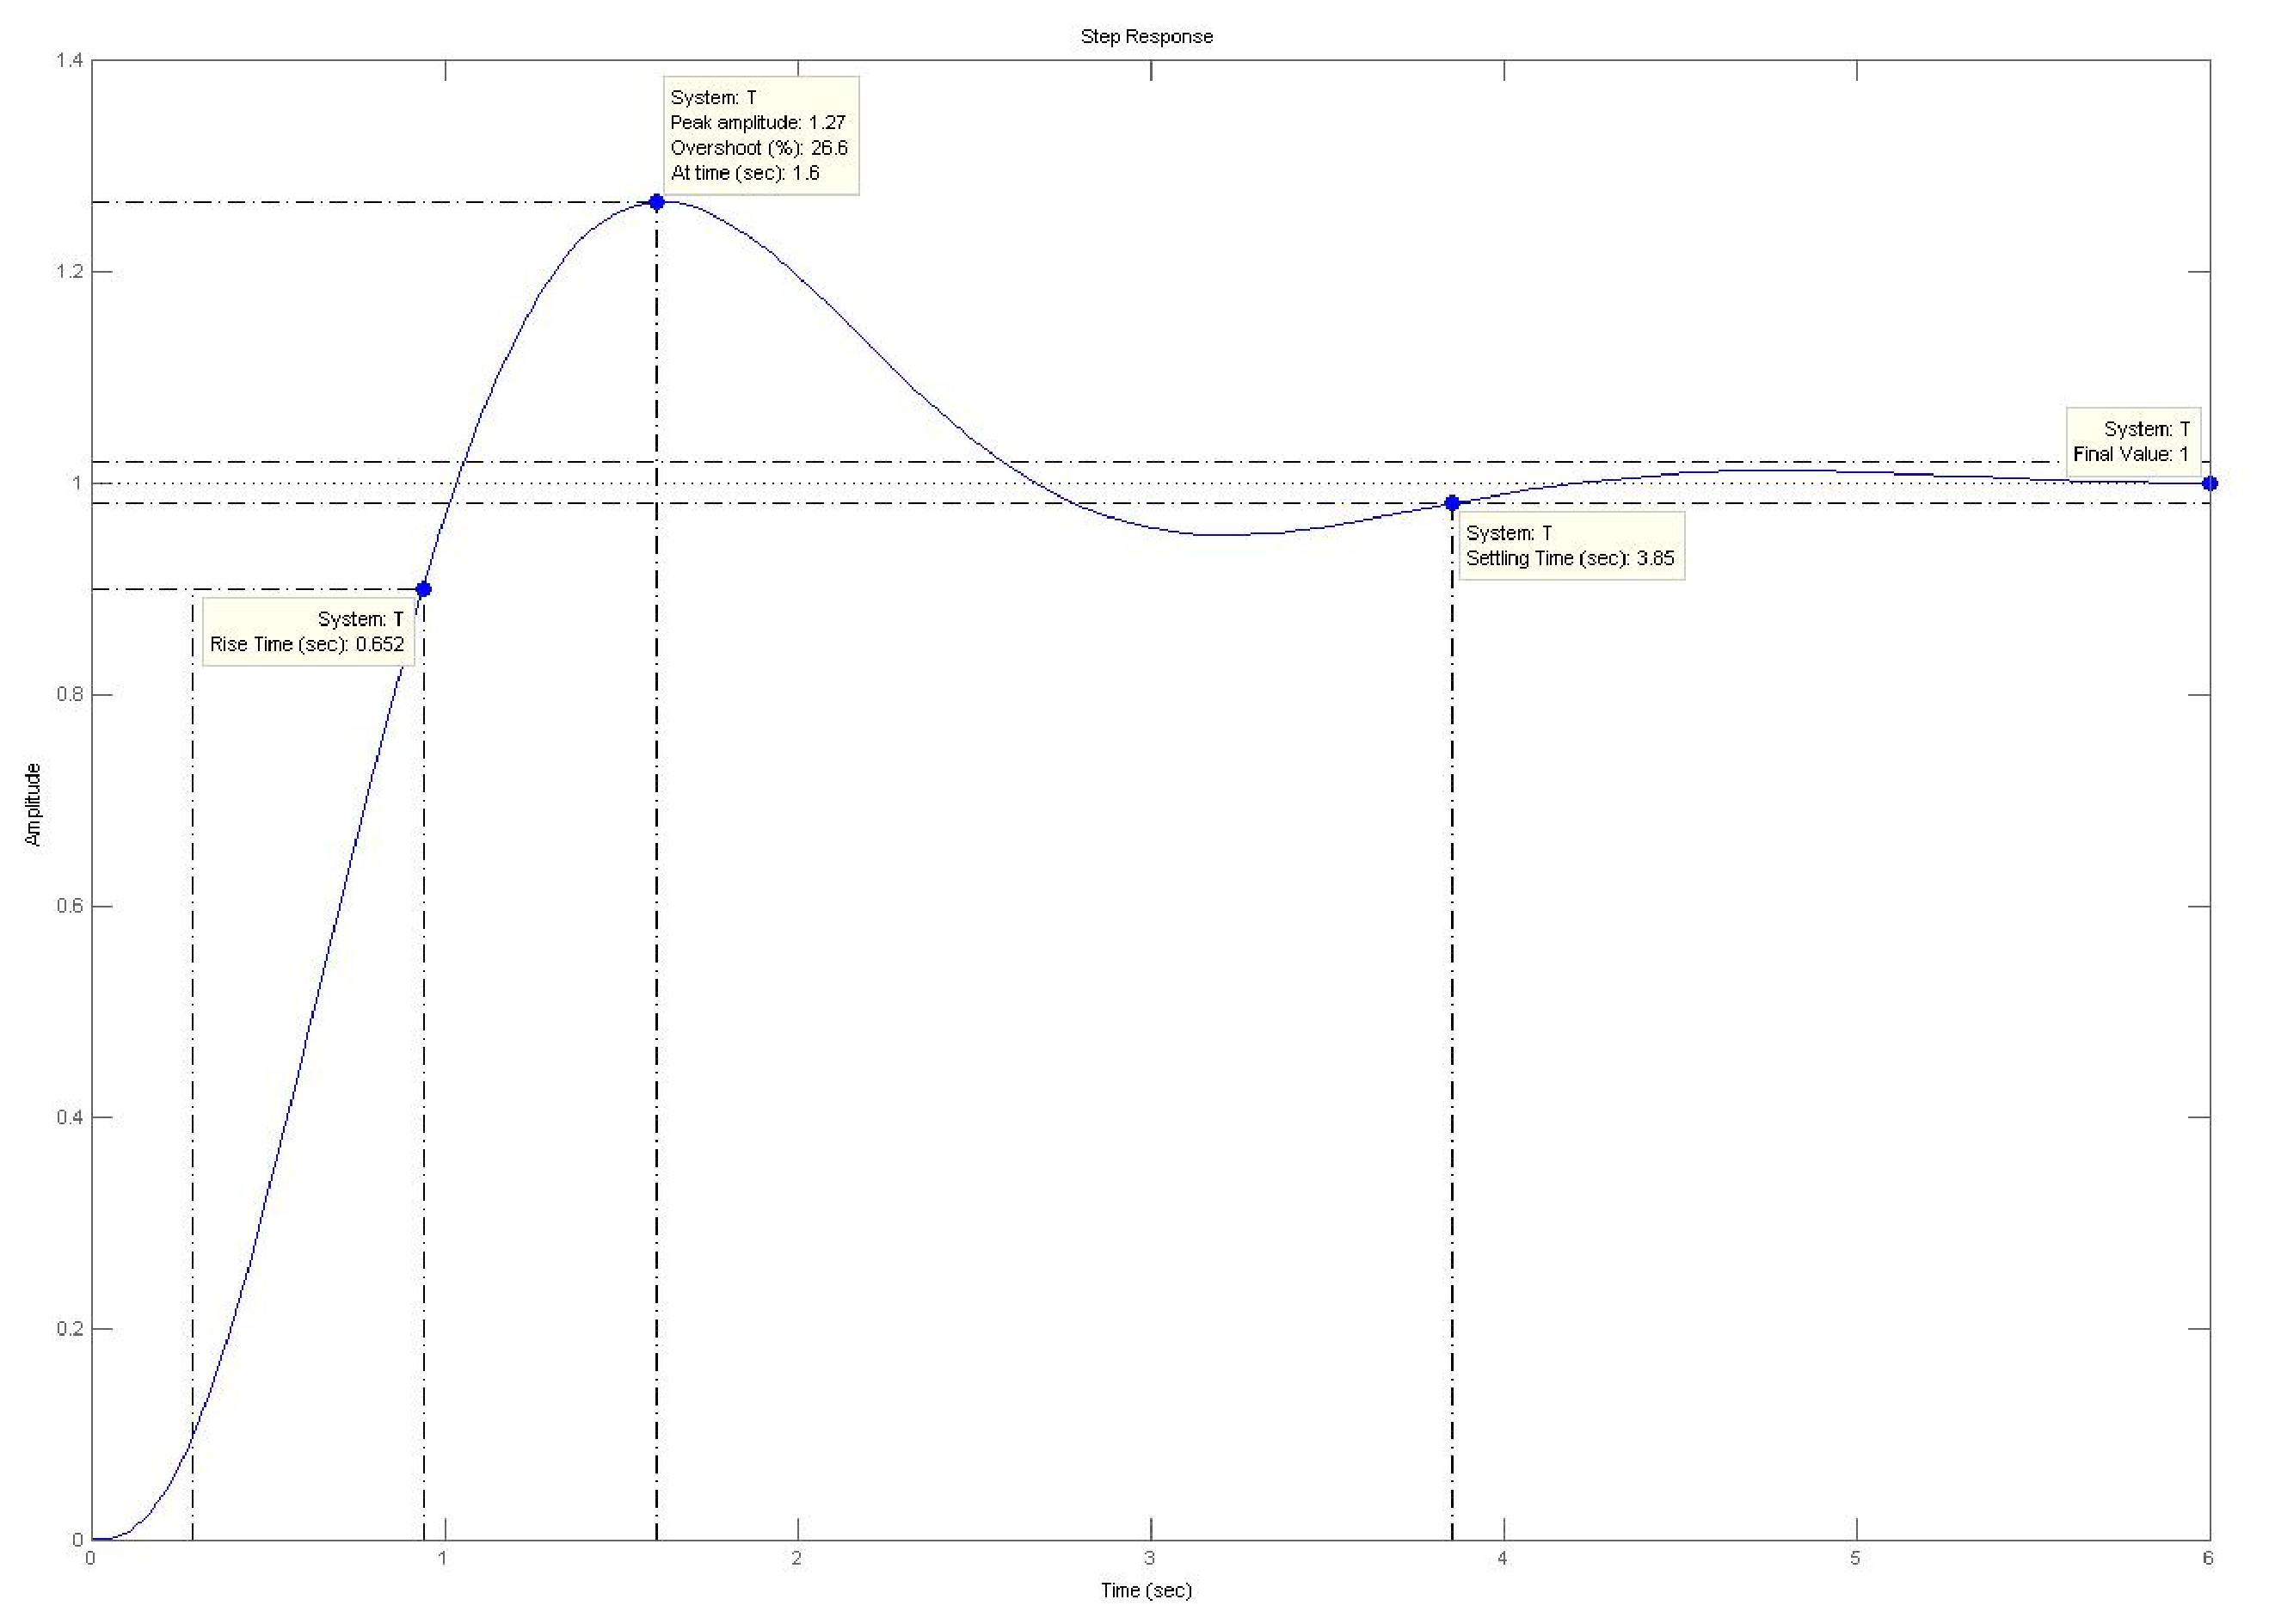
\includegraphics[width=.9\textwidth]{ltiviewstep}
\caption{ \footnotesize
        Step response with metadata tags for Example~\ref{ex.ltiview}
        \label{fig.ex.ltiviewstep}
        }
\end{figure}
\par
For time-domain analysis, it is often much easier to use the LTI Viewer because it is possible to obtain many system parameters with a simple right-click of the mouse.  In addition, it allows us to select from a myriad of responses and data projections via the Plot Type.

\subsection{Numerical Solutions of Differential Equations}
There are many powerful techniques in MATLAB for the numerical solution of nonlinear equations.  A popular technique is the Runge-Kutta method, which is based on formulas derived by using an approximation to replace the truncated Taylor series expansion.  The interested reader should see \cite{butcher} or an equivalent text on numerical methods.
\par
MATLAB provides several powerful functions for the numerical solution of differential equations: See Table~\ref{tab.odesolvers}.  Two of the functions employing the Runge-Kutta-Fehlberg methods are \verb=ode23= and \verb=ode45=; they are based on the Fehlberg second- and third-order pair of formulas for medium accuracy and the fourth- and fifth-order pair for higher accuracy.

\begin{table}[bht]
\centering
\renewcommand{\arraystretch}{1.2}
\begin{tabular}{c|p{0.55\textwidth}}
    \textit{Command}& \multicolumn{1}{c}{\textit{Description}}\\ \hline \hline
    \verb=ode23=        &   Solve non-stiff differential equations,
                                low order method \\
    \verb=ode45=        &   Solve non-stiff differential equations,
                                medium order method
\end{tabular}
\caption{\footnotesize
        Numerical solvers for ordinary differential equations
        \label{tab.odesolvers}
        }
\end{table}
\par
The $n^{th}$-order differential equation must be transformed first into $n$ first-order differential equations and must be placed in an m-file that returns the derivative of the state equations.  This file's name is represented as the string \verb='xprime'= in the general syntax below:
\begin{verbatim}
[t, x] = ode23('xprime',tspan,x0,option)
\end{verbatim}
Also, \verb=tspan= is a vector of times covering the interval of integration, and \verb=x0= is a column vector of initial state conditions.  Commonly used options are scalar relative error tolerance (\verb#RelTol = 1e-3# by default) and vector absolute error tolerances (all elements of \verb#AbsTol = 1e-6# by default).

\begin{workex}  \label{ex.ode23}
\begin{equation*}
    \frac{d^2\theta}{dt^2} + \frac{B}{m} \frac{d\theta}{dt} +
        \frac{g}{l} \sin \theta = 0
\end{equation*}
The above equation describes the motion of the simple pendulum derived in Lab Session \ref{ch.ModSim}, Case Study \ref{cs.simplepend}.  Using the MATLAB function \verb=ode23=, obtain the numerical solution for the following values:
\begin{itemize}
    \item $m = 0.5$kg and $l = 0.613$m
    \item $B = 0.05$kg-s/m and $g = 9.81$m/s/s
    \item $\theta(t=0) = \dot{\theta}(t=0) = 0$
\end{itemize}

\end{workex}


\begin{thebibliography}{9}
    \bibitem{dorf} Richard C. Dorf and Robert H. Bishop.  Modern Control Systems, 11th edition.  Prentice Hall, Upper Saddle River, NJ.  2008.
    \bibitem{firsted} EE351L Laboratory Manual, 1st edition.
    \bibitem{butcher} John C. Butcher.  Numerical Methods for Ordinary Differential Equations, 2nd edition.  John Wiley.  2003.
\end{thebibliography}

% Appendix
% Worked Solutions

\chapter{Worked Solutions}

\section{Lab \ref{ch.Matlab}}
\input{MatlabSolutions}
\section{Lab \ref{ch.StaVar}}
\input{StaVarSolutions}
\section{Lab \ref{ch.ModSim}}
\input{ModSimSolutions}
\section{Lab \ref{ch.PosCon}}
\begin{Solution}{1}
        The block diagram can be constructed by simply writing the pertinent equations one after the other and labeling the intermediate signals.  The full diagram should look something like Fig.\ \ref{fig.sol.poscon.blockdiagram}.
        \begin{figure}
        \centering
        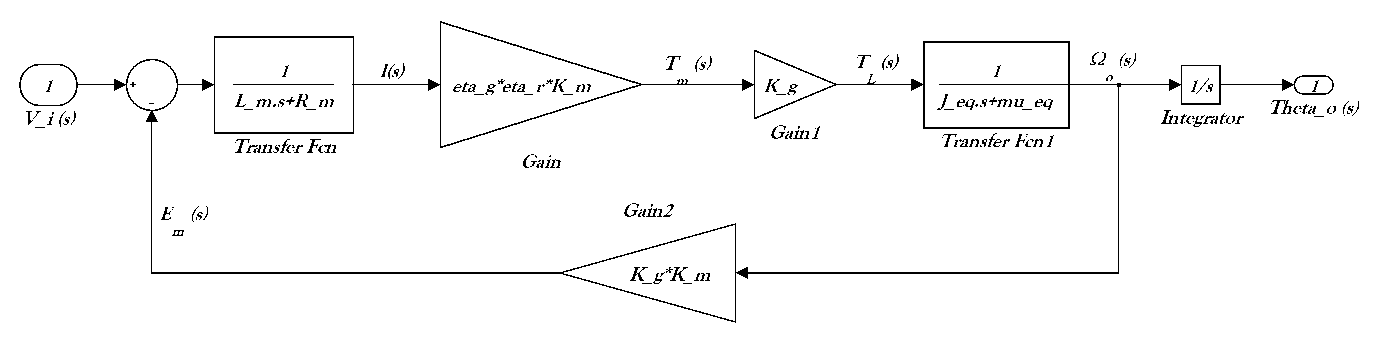
\includegraphics[angle=90, height=.95\textheight]{posconprelab1}
        \caption{\label{fig.sol.poscon.blockdiagram}}
        \end{figure}
        
\end{Solution}
\begin{Solution}{2}
        From the block diagram in question 1, it is a matter of reducing it to a single transfer function.  Use the rule that a negative feedback loop with block $G_1$ in the forward path and $G_2$ in the reverse path reduces to
        \begin{equation}
            G = \frac{G_1}{1+G_1G_2}
        \end{equation}
        After setting $L_m=0$, we have
        \begin{equation}
            TF_{V_i\to\Omega_o} =
                \frac{\frac{\eta K_m K_g}{R_m} \frac{1}{\mu_{eq} + J_{eq}s}}{ 1 + K_g K_m \frac{\eta K_m K_g}{R_m} \frac{1}{\mu_{eq} + J_{eq}s}}
        \end{equation}
        Note that $\eta := \eta_g \eta_r$.  To simplify, we multiply top and bottom of the big fraction by $\mu_{eq} + J_{eq}s$ to get
        \begin{equation}
            = \frac{
                    \frac{
                            \eta K_m K_g
                            }{
                            R_m
                            }
                    }{
                    \mu_{eq} + J_{eq}s + \frac{
                                                \eta K_m^2 K_g^2
                                                }{
                                                R_m
                                                }
                    }
        \end{equation}
        And now multiplying top and bottom by $1/J_{eq}$, we arrive at
        \begin{equation}
            = \frac{
                    \frac{
                            \eta K_m K_g
                            }{
                            R_m J_{eq}
                            }
                    }{
                    s + \frac{
                                \mu_{eq}
                                }{
                                J_{eq}
                                }
                    + \frac{
                            \eta K_m^2 K_g^2
                            }{
                            R_m J_{eq}
                            }
                    }
        \end{equation}
        Thus we have the correct form with pole-zero constants:
        \begin{subequations}
        \begin{gather}
            a = \frac{\eta K_m K_g}{R_m J_{eq}} \approx 288.3844\\
            b = \frac{\mu_{eq}}{J_{eq}} + \frac{\eta K_m^2 K_g^2}{R_m J_{eq}}
                \approx 40.4091
        \end{gather}
        \end{subequations}
        \par
        Finally, to get the TF to output position, we only need to pass the above TF through an integrator (it will have the same constants $a$ and $b$):
        \begin{equation}
            TF_{V_i\to\Theta_o} =
                \frac{a}{s(s+b)}
        \end{equation}
    
\end{Solution}
\begin{Solution}{3}
        The FVT looks like
        \begin{equation}
            \lim_{t\to\infty} \theta_o(t) = \lim_{s\to0}s\Theta_o(s)
        \end{equation}
        Applying this to our system, we have
        \begin{equation}
            \lim_{t\to\infty} \theta_o(t)
            =
            \lim_{s\to0} s \frac{1}{s} \frac{a}{s(s+b)} = \infty
        \end{equation}
        Some explanation:  The leading $s$ comes from the FVT itself.  The $1/s$ gives the systems response to a step input.  The rest of the expression is simply the transfer function to output position found in Question 2.
        
\end{Solution}
\begin{Solution}{4}
        The inner feedback loop (the derivative control) in Fig.\ \ref{fig.servoPD} can be reduced to
        \begin{equation}
            G_1(s) := \frac{
                            \frac{a}{s+b}
                            }{
                            1+K_D\frac{a}{s+b}
                            }
        \end{equation}
        Then in the forward path of the remaining diagram, we have $K_P G_1(s)/s$.  The remaining diagram is a simple unity feedback system:
        \begin{equation}
            TF_{\Theta_i\to\Theta_o} :=
            \frac{K_P G_1(s)/s}{1+K_P G_1(s)/s}
                \label{eq.servoPDtf}
        \end{equation}
        Simplifying Equation~(\ref{eq.servoPDtf}) yields the classical second-order transfer function:
        \begin{equation}
            TF_{\Theta_i\to\Theta_o} =
            \frac{
                K_P a
                }{
                s^2 + s(b+K_D a) + K_P a
                }
                \label{eq.servoPD}
        \end{equation}
        
\end{Solution}
\begin{Solution}{5}
        Comparing Eqs.\ (\ref{eq.secondordertf}) and (\ref{eq.servoPD}), we can conclude the following basic parameters:
        \begin{subequations}
        \begin{flalign}
        K &= 1 \\
        \omega_n &= \sqrt{K_P a} \\
        \zeta &= \frac{b+K_D a}{2\sqrt{K_P a}} \label{eq.servoDR}
        \end{flalign}
        \end{subequations}
        We then translate the formula given for peak time into one with our parameters:
        \begin{equation}
        t_p =  \frac{\pi}{\omega_n \sqrt{1-\zeta^2}}
        = \frac{
                \pi
                }{
                \sqrt{K_P a}\sqrt{1-\frac{
                                        (b+K_D a)^2
                                        }{
                                        4K_P a
                                        }
                                        }
                }
            \label{eq.servoPT}
        \end{equation}
        Now we have a system of equations with two unknowns ($K_P$, and $K_D$) and two equations (\ref{eq.servoDR} and \ref{eq.servoPT}).  You can solve these using your favorite method.  One way would be to rearrange Eq.\ \ref{eq.servoDR} for $K_D$ and then substitute into Eq.\ \ref{eq.servoPT} to solve for $K_P$ first.  Using $K_P$, you can then go back and find $K_D$.
        \par
        These parameters turn out to be:
        \begin{flalign*}
            K_P &\approx 27.3708 \\
            K_D &\approx 0.2955
        \end{flalign*}
        
\end{Solution}
\begin{Solution}{6}
        The solution to this question is provided in Fig.\ \ref{fig.servoPDmodel}.
        
\end{Solution}


\end{document}

